\pagestyle{empty}
\graphicspath{{Factor_organizativo/}}
\part{El factor organizativo}

.. _Factor_organizativo:

\onecolumn

\sffamily

\vspace*{4cm}

En esta parte se tratar�n las ideas relacionadas con la organizaci�n y estructuraci�n del sistema SIG, desarrollando los aspectos sociales tanto a nivel t�cnico como funcional.



* El cap�tulo \ref{Introduccion_factor_organizativo} desarrolla la importancia del factor organizativo en un SIG, presentando las principales elementos que van a permitir una correcta organizaci�n y relaci�n entre elementos del SIG. Se trata conjuntamente todo lo relativo a la implementaci�n de un SIG, siguiendo las pautas de organizaci�n presentadas.

%* El cap�tulo \ref{Implantacion} estudia el proceso de implementaci�n de un SIG y los aspectos que deben considerarse para que este sea exitoso.

* En el cap�tulo \ref{IDEs} se explicar�n los conceptos b�sicos sobre las Infraestructuras de Datos Espaciales, con el objetivo de introducir las principales caracter�sticas que las conforman y la nueva forma de trabajar que su uso conlleva. Veremos, asimismo, los principales acuerdos que tanto a nivel nacional como internacional se han tomado para su correcto desarrollo y funcionamiento.

* Un elemento fundamental para gestionar los datos son los denominados *metadatos*. El cap�tulo \ref{Metadatos} est� dedicado por entero a ellos, describiendo la importancia que tienen en el contexto actual de los SIG.

* A lo largo del cap�tulo \ref{Estandares} se tratan los principales est�ndares existentes en el campo de la informaci�n geogr�fica y los servicios que estos definen, analizando sus especificaciones y su importancia.




\rmfamily
%\twocolumn

\chapter{Introducci�n. �C�mo se organiza un SIG?}\label{Introduccion_factor_organizativo}
\pagestyle{fancy}

\begin{keypoints}
�C�mo se organizan los distintos elementos del sistema SIG? $\bullet$ �Por qu� es necesario planificar una correcta organizaci�n dentro de un SIG? $\bullet$ �Qu� criterios deben seguirse para llevar a cabo esa organizaci�n?$\bullet$�Qu� debemos considerar antes de comenzar a trabajar con un SIG?
\end{keypoints}

\bigskip

\begin{intro}
Trabajar con un SIG requiere una correcta organizaci�n a todos los niveles. Ahora que conocemos qu� podemos hacer con un SIG, es el momento de ver c�mo debemos plantearnos ese trabajo de forma �ptima, dejando los aspectos t�cnicos y centr�ndonos en aspectos funcionales, organizativos y humanos, todos ellos igual de importantes que los anteriores ya vistos.

En este cap�tulo se presentan las ideas fundamentales relativas a la organizaci�n de un SIG, su implantaci�n y uso. Estas ideas ser�n b�sicas para entender posteriormente los restantes cap�tulos de esta parte, en los que se desarrollan por separado algunos conceptos relacionados y de gran importancia en la escena actual de los SIG.
\end{intro}

\section{Introducci�n}

Como sistema complejo, un SIG requiere una organizaci�n eficiente que permita la correcta interacci�n de todos sus elementos y a todos los niveles. Esta organizaci�n es tanto m�s necesaria cuanto m�s volumen adquiere el sistema SIG, pues la propia complejidad de este puede conllevar la perdida de eficiencia y un uso en el que no se aprovechan plenamente las capacidades que el SIG ofrece como herramienta para el trabajo con datos geogr�ficos. Una organizaci�n ineficiente es con frecuencia el cuello de botella m�s importante con el que un sistema SIG se encuentra y, parad�jicamente, un aspecto con frecuencia olvidado.

Los niveles de complejidad y volumen que encontramos actualmente en el �mbito de los SIG son muy superiores a los que exist�an hace apenas unos a�os, y requieren un enfoque distinto para poder lograr que todas las piezas del SIG funcionen de forma armoniosa y sincronizada, sin problemas derivados de una mala sincronizaci�n o de un incorrecto dimensionamiento del sistema. De hecho, el cambio que ve�amos en el cap�tulo \ref{Introduccion_fundamentos} en la definici�n del propio SIG, en el que se pasaba de una combinaci�n de \emph{hardware} y \emph{software} para manejo de datos localizados espacialmente a un sistema complejo con m�s componentes, viene en gran medida desencadenado por la creciente consideraci�n de la organizaci�n como un factor vital para el buen funcionamiento del SIG. Esa organizaci�n a la que originalmente no se le conced�a la relevancia actual debido a que las circunstancias eran distintas, se ha demostrado en el contexto presente como un elemento clave para la gesti�n del SIG, y sin duda alguna un elemento al que ha de prestarse atenci�n en cualquier utilizaci�n de un SIG m�s all� del �mbito meramente personal.

Implantar un SIG (es decir, establecer un entorno SIG susceptible de ser empleado productivamente) es una labor compleja. No basta con conseguir un \emph{software} SIG, instalarlo en un ordenador, conseguir un conjunto de datos y ponerse a trabajar para dar respuestas a un problema dado en el que se requiera alg�n tipo de an�lisis geogr�fico. Ni siquiera en el supuesto de un contexto individual de trabajo ---la expresi�n m�nima que podemos encontrar, y por tanto la m�s sencilla de gestionar--- la implantaci�n resulta tan sencilla, ya que deben considerarse algunos aspectos antes de llevar a cabo cualquier acci�n. En este cap�tulo, vamos a ver cu�les son los puntos m�s importantes en los que debemos recalar a la hora de implantar un SIG, de forma que garanticemos el buen funcionamiento de este y establezcamos las condiciones adecuadas para poder trabajar con dicho SIG de forma �ptima.

Las ideas de este cap�tulo son de inter�s no solo para los encargados de implantar como tal el SIG y ponerlo en funcionamiento dentro de un determinado entorno, sino para todo aquel usuario o persona implicada de alg�n modo en ese entorno. De un modo u otro, resulta interesante conocer las reglas que regulan el funcionamiento del sistema si se es en cierta medida parte de �l. M�s a�n, el trabajo con un SIG no solo incluye la utilizaci�n directa de este, sino tambi�n un cierto planeamiento de ese trabajo y una serie de tomas de decisiones previas. Estas consideraciones, que aparecen en la realizaci�n de cualquier proyecto con independencia de su �ndole, afectan tambi�n a los Sistemas de Informaci�n Geogr�fica, y ser� en este aspecto en el que profundizaremos a lo largo de este cap�tulo.

\section{La importancia de la organizaci�n}

Hemos citado ya la importancia de la organizaci�n dentro de un SIG, justificando as� brevemente la conveniencia de estudiar la mejor forma posible de llevar esta a cabo. Veamos con m�s detalle el porqu� de dicha importancia y las consecuencias directas que una adecuada implantaci�n de un SIG tiene en el funcionamiento de este y, especialmente, en su eficacia, rendimiento y en la calidad del trabajo realizado con �l. Las siguientes son las dos principales de ellas:

\begin{itemize}
	\item Mejor relaci�n entre elementos del sistema. El sistema no lo componen �nicamente un conjunto de elementos, sino tambi�n una serie de relaciones dentro del sistema. Si estas relaciones son fluidas y existe una sinergia entre las funciones que cada parte cumple en el todo del sistema, el funcionamiento de este �ltimo sera mejor. 
	
	En el sistema representado por un SIG, algunos elementos como los datos son utilizados por todos los restantes. El dise�o de este elemento debe tener en cuenta esa circunstancia para que no existan problemas al interactuar con otras partes del SIG, como pueden ser las personas o el \emph{hardware} y \emph{software} empleado. El \emph{hardware} debe dimensionarse para tener capacidad suficiente a la hora de manejar los vol�menes de datos con los que se trabaja, y el \emph{software} debe ser capaz de poder acceder a los datos en el formato en que estos se encuentren almacenados. Por su parte, los datos deben ser los adecuados para satisfacer las necesidades de los usuarios que forman parte del sistema, para que estos, a trav�s de los procesos de an�lisis y otras operaciones disponibles, obtengan resultados de inter�s de una forma �ptima. Consideraciones similares pueden realizarse si se consideran elementos distintos del sistema SIG y su interrelaci�n particular.
	\item Mejor relaci�n entre representantes de un mismo elemento del sistema. Los elementos del sistema son a su vez conjuntos de otros elementos. La parte humana de un SIG no es una �nica persona, del mismo modo que el \emph{software} puede no ser una �nica aplicaci�n, sino varias de ellas para realizar distintas tareas sobre la informaci�n geogr�fica. A medida que avanzamos en el desarrollo de los SIG, encontramos escenarios m�s complejos en los que se multiplica la magnitud de los distintos factores implicados (m�s gente, m�s datos, m�s potencia en el \emph{hardware} empleado...), requiri�ndose a su vez una organizaci�n interna de esos mismos factores.
	
	A la hora de planificar la implantaci�n de un SIG, debemos tratar de homogeneizar internamente cada uno de sus elementos, o al menos de incorporar mecanismos que garanticen una correcta comunicaci�n y coordinaci�n a todos los niveles. Esto puede implicar, por ejemplo, aplicar estrategias de trabajo coordinado para organizar el factor humano, o emplear esquemas comunes para el almacenamiento de datos. Si cada uno de los datos con que trabajamos presenta una estructura distinta, encontraremos el mismo problema que si las distintas personas que van a trabajar en nuestro entorno SIG hablan distintos idiomas y son incapaces de comunicarse. En esta situaci�n, puede resultar complejo y poco eficiente (o incluso ser por completo imposible) emplear varios grupos de datos de forma conjunta, restando as� capacidades y eficiencia al sistema. 
\end{itemize}

Logrando lo anterior, el sistema SIG ofrece mejor funcionamiento, justificando as� plenamente el esfuerzo desarrollado para su correcta implementaci�n y organizaci�n, esfuerzo que, por otra parte, en ocasiones es notable y no debe menospreciarse.

\section{Organizando los distintos elementos de un SIG}

Ahora que ya sabemos por qu� es importante una adecuada organizaci�n de un SIG, veamos algunas ideas b�sicas sobre la forma de lograr esta. Para ello, y puesto que la organizaci�n es un concepto �ntimamente ligado a la estructura del SIG como sistema, veremos por separado c�mo plantear esa organizaci�n para los principales elementos de este, los cuales ya conocemos bien de cap�tulos anteriores. Descubriremos as� que la implantaci�n de un SIG es mucho m�s que simplemente elegir una aplicaci�n y utilizarla, y que una implantaci�n que no cubra todos los aspectos fundamentales que a continuaci�n detallaremos es muy probable que presente problemas y falle a la hora de ofrecer respuestas a las necesidades a las que un SIG correctamente planificado puede responder.

\subsection{Datos}

Ya sabemos que sin datos no podemos trabajar en un SIG, por lo que la implantaci�n de este implica necesariamente la implantaci�n de un conjunto de datos a partir de los cuales poder efectuar las operaciones propias del SIG. Esto conlleva el dise�o y creaci�n de una base de datos contra la que posteriormente trabajar�n las distintas aplicaciones, bien sea para leer esos datos, modificarlos, o a�adir nuevos datos.

A la hora de planificar el dise�o y creaci�n de la base de datos, se deben considerar todas las actividades que a lo largo de su vida van a desarrollarse sobre ella. En funci�n de esto, se establecen las distintas etapas a seguir, que en una primera aproximaci�n pueden ser las siguientes:

\begin{itemize}
	\item Recopilaci�n de datos. Los datos a incluir en nuestro SIG pueden obtenerse de procedencias muy diversas, ya sea adquiri�ndolos de proveedores privados, de organismos oficiales o de cualquier otra entidad que disponga de los datos que van a ser necesarios. La elaboraci�n de una lista de datos necesarios ha de realizarse considerando los futuros an�lisis que tendr�n lugar sobre ellos, con objeto de saber qu� datos hemos de obtener (es decir, qu� variables del medio van a ser necesarias), pero tambi�n algunas caracter�sticas m�s detalladas de esos datos. Por ejemplo, si los usuarios de nuestro SIG van a hacer estudios a distintas escalas, es de inter�s contar con un mismo dato en esas escalas de trabajo, para as� facilitar el manejo de datos y optimizar las operaciones.
	
	Si los datos que pueden obtenerse por las v�as habituales no son suficientes, ser� necesario, siempre que ello sea viable dentro del contexto de la implantaci�n, elaborar aquellos que no hayan podido obtenerse. La creaci�n de estos datos debe encaminarse a obtener un producto acorde con el resto de datos de que disponemos, para que puedan integrarse de la forma m�s sencilla posible y disminuyan el trabajo a realizar.
	
	En ocasiones, la creaci�n de nuevos datos no implica obligatoriamente el desarrollo de trabajo de campo o la aplicaci�n de t�cnicas como las que vimos en el cap�tulo \ref{Fuentes_datos} (por ejemplo, la digitalizaci�n). Puede ser interesante elaborar nuevas capas de datos a partir de las ya disponibles, mediante procesos de an�lisis u operaciones como las que hemos visto en la parte \ref{Procesos} de este libro. Aunque estos procesos pueden ser llevados a cabo por los usuarios en el momento de necesitar un determinado dato, crear previamente ese dato y ofrecerlo junto a los dem�s puede ser interesante por varias razones. 
	
	En primer lugar, si son varios los usuarios que en un momento concreto van a necesitar ese dato, evitaremos la repetici�n innecesaria del proceso, con la consiguiente ganancia de tiempo. En segundo lugar, un usuario puede no estar capacitado o no disponer de la experiencia necesaria para crear correctamente ese dato, especialmente si el proceso a seguir es complejo o proclive a la aparici�n de errores. El hecho de que un usuario necesite un dato no implica que conozca la forma de elaborarlo a partir de otros datos primarios.
	
	\item Preparaci�n de los datos. Obtener los datos es solo la mitad del trabajo. Si creamos nuestra base de datos con los datos que hemos adquirido tal y como han sido suministrados, es probable que el trabajo posterior sea dif�cil y complejo. Salvo que todos los datos provengan de un �nico proveedor, vamos a tener datos con una gran heterogeneidad, la cual no favorece en absoluto el trabajo fluido con ellos. Incluso si todos los datos tienen un origen com�n, es necesario prepararlos para el uso particular que esperamos se realice en nuestro SIG, teniendo en cuenta aspectos que no han sido considerados por el proveedor. 
	Los siguientes son algunos de los apartados a los que debe prestarse atenci�n para la preparaci�n de datos:
	
\begin{itemize}
	\item Extensi�n geogr�fica. Algunos datos pueden cubrir una regi�n mucho mayor que la que se espera vaya a ser necesaria en el desarrollo de proyectos dentro de nuestro SIG. En tal caso, <<recortar>> la extensi�n disminuye el volumen de datos y facilita su manejo.
	\item Formato. El formato debe ser el adecuado para que las aplicaciones puedan leer los datos, lo cual no siempre sucede. Cada proveedor de datos suele tener unas pautas a la hora de distribuir sus datos, y esto puede no coincidir con las capacidades de lectura de datos del \emph{software} que vamos a utilizar. En tal caso, es necesaria una conversi�n de formato para que los usuarios no encuentren dificultades en ese sentido.
	\item Modelo de datos. La forma en que esta recogida la informaci�n geogr�fica define en gran medida lo que podemos hacer con ella una vez la incorporemos al SIG, como vimos en el cap�tulo \ref{Tipos_datos}. Si, por ejemplo, sabemos que una gran parte del trabajo en nuestro SIG va a implicar el an�lisis de Modelos Digitales de Elevaciones, este se lleva a cabo mayoritariamente sobre capas r�ster, tal y como explicamos en el cap�tulo \ref{Geomorfometria}. Si disponemos de una capa de elevaciones recogida como un conjunto de curvas de nivel (es decir, una capa vectorial), resulta conveniente transformar esta y que exista en el conjunto de datos del SIG un MDE r�ster, mucho m�s acorde con lo que los usuarios van a requerir.\index{Modelo Digital de Elevaciones}
	\item Sistema de coordenadas. Si los datos tienen distintos sistemas de coordenadas, ser� necesario transformarlos a un sistema com�n, preferentemente a aquel que vaya a ser utilizado con m�s frecuencia para la generaci�n de resultados.\index{Coordenadas!sistemas de}
	\end{itemize}
	
\end{itemize}


En resumen, el objetivo principal que debemos perseguir al configurar el conjunto de datos que van a formar parte de un SIG es lograr que la utilizaci�n de estos sea lo m�s sencilla y fluida posible. Un conjunto de datos rico y variado, bien estructurado y cuyo empleo no d� lugar a problemas o haga aparecer necesidades adicionales, simplificar� m�s tarde el trabajo con el SIG y ser� una garant�a del �xito de su implementaci�n.

\subsection{Personas}

Si a lo largo de este libro hemos mencionado en repetidas ocasiones que los datos son el elemento imprescindible del sistema SIG, a la hora de implementar y organizar este son las personas quienes juegan el papel principal. El desarrollo del sistema SIG debe realizarse a partir de los usuarios, ya que la influencia que tienen en los restantes elementos es muy superior a la de estos otros. Los usuarios son quienes operan directamente con las aplicaciones y quienes adem�s han de tomar decisiones a lo largo de un proyecto SIG, por lo que es necesario escuchar sus necesidades y sus opiniones antes de implantar un SIG, con el fin de proporcionarles el mejor entorno posible.

Las consideraciones acerca de los restantes elementos, tales como datos o \emph{software}, deben matizarse <<escuchando>> lo que los usuarios pueden decir al respecto. El �xito en la implantaci�n de un SIG pasa por tener en cuenta de forma conjunta los requerimientos del mayor n�mero de usuarios posible, considerando incluso el perfil de futuros usuarios que puedan incorporarse m�s adelante.

Resulta err�neo, por ejemplo, adquirir un determinado \emph{software} bas�ndose exclusivamente en las propias caracter�sticas de este, y sin consultar a los futuros usuarios si poseen alguna experiencia previa con �l o con otro similar. No siempre la mejor herramienta desde el punto de vista t�cnico garantiza unos mejores resultados al usarla, ya que existen otros factores que afectan a la productividad y la calidad de los trabajos que se desarrollen posteriormente sobre esa herramienta. 

Una sencilla encuesta a los usuarios es una herramienta muy valiosa para aportar informaci�n en este sentido y decantar la elecci�n de la herramienta en uno u otro sentido. Igualmente, nos permitir� saber algo m�s sobre el nivel medio de los usuarios, sus preferencias o el tipo de trabajo que desarrollan mayoritariamente.

Se admite generalmente que el �xito en la implantaci�n de un SIG pasa por un modelo de implantaci�n que d� preponderancia a los usuarios como factores a considerar. No obstante, este enfoque no es siempre sencillo y no siempre est� exento de riesgos. Definir las necesidades de los usuarios es uno de los aspectos vitales para la implementaci�n de un SIG, pero tambi�n uno de los m�s dif�ciles \cite{Campbell1992IJGIS}. En ocasiones, por ejemplo, el usuario no necesariamente sabe qu� es lo que necesita o qu� le conviene. Un problema muy habitual en el mundo del SIG es el desconocimiento por parte de los usuarios de las verdaderas capacidades que el SIG tiene y puede ofrecerles. Estos usuarios son capaces de utilizar un SIG, pero el aprovechamiento que hacen de este no es �ptimo, ya que ignoran una gran parte de su potencia. El hecho de que las aplicaciones SIG sean complejas y dispongan de funcionalidades numerosas contribuye a este hecho.

En este sentido, es importante considerar el papel de los usuarios tambi�n con posterioridad a la implantaci�n del SIG, es decir, una vez que se ha tomado una decisi�n acerca de otros elementos como \emph{software} o datos, y estos ya se encuentran operativos. En lo que al \emph{software} respecta, esto incluye el desarrollo de acciones tales como seminarios o presentaciones, que divulguen las capacidades del SIG entre los usuarios y les hagan conscientes de lo que pueden lograr con este.

Otro de los aspectos importantes en el elemento formado por los usuarios son las relaciones entre estos. Cit�bamos como una de las ventajas de una buena organizaci�n el hecho de que existe un mejor conexi�n no solo entre los distintos elementos del SIG, sino tambi�n en cada uno de dichos elementos, entre sus distintos representantes. Esto es especialmente relevante en el caso de los usuarios, ya que la comunicaci�n fluida entre ellos puede evitar muchos problemas y aumentar sensiblemente la productividad y la calidad del trabajo. Los usuarios con mayor experiencia pueden solucionar problemas a usuarios menos experimentados, aconsejarles en el desarrollo de su trabajo o instruirles en las capacidades del \emph{software}. La creaci�n de comunidades de usuarios activas es una buena se�al de una implantaci�n exitosa de un SIG, y estas comunidades pueden incluso trascender el �mbito de una implantaci�n particular de un SIG, extendi�ndose hasta cubrir a todos los usuarios de una determinada aplicaci�n, o a todos los involucrados en un �rea de conocimiento dada en la que se utilice un SIG.


Por �ltimo, es importante para definir las necesidades de los usuarios saber clasificar a estos y conocer su papel en el SIG. Un usuario puede tener funciones muy distintas, ya que consideramos como tal a toda persona involucrada en el sistema SIG, no exclusivamente a aquellas que directamente realizan el trabajo m�s t�pico tal como el an�lisis de datos y la obtenci�n de cartograf�a a partir de ese an�lisis. Para ver esto, podemos acudir a un ejemplo sencillo.

Volvamos al caso presentado en el primer cap�tulo de este libro, relativo a la gesti�n de una masa forestal, y analicemos qu� tipos de usuarios podemos encontrar y el papel que cada uno de ellos desarrolla en el SIG.

En un extremo encontramos a las personas encargadas de la toma de decisiones, tales como los gestores y miembros de la administraci�n responsable de la masa forestal. Estas personas no han de tener necesariamente unos amplios conocimientos de SIG, sino tan solo ser capaces de entender los resultados que se generan con este. En funci�n de ellos, tomar�n decisiones aplicando su experiencia al respecto, que en este �rea s� que debe ser elevada. En una posici�n similar encontramos a los operarios encargados del trabajo de campo y agentes forestales que trabajan directamente sobre la masa, y que, en t�rminos del SIG, realizan fundamentalmente una labor de recogida de datos. Deben conocer bien el entorno forestal y las t�cnicas de muestreo y toma de datos, pero no es un requisito imprescindible que cuenten con experiencia en SIG. Si la recogida se realiza empleando alguna tecnolog�a a tal efecto, o incluso alg�n tipo de SIG sobre una plataforma m�vil, deber�n tener nociones b�sicas de manejo, pero eso no constituye un conocimiento amplio de los SIG y sus capacidades.

En el extremo contrario a los anteriores encontramos a aquellos usuarios que se encargan de las cuestiones m�s t�cnicas del SIG y de corte m�s inform�tico. Entre ellos est�n los administradores de las bases de datos, los programadores o los t�cnicos encargados de la digitalizaci�n de cartograf�a. Estos deben tener un amplio conocimiento del \emph{software} que usan, pero no es necesario que sean expertos en el �mbito de aplicaci�n en el que se encuentran. As�, los t�cnicos que digitalicen cartograf�a deben tener suficientes conocimientos cartogr�ficos y de manejo de la herramienta, pero pueden desarrollar su trabajo sin conocer en profundidad aquello que est�n digitalizando (por ejemplo, parcelas de inventario o unidades de gesti�n del monte).

Entre estos dos extremos encontramos un diverso abanico de usuarios que emplear�n de un modo u otro el SIG, y que aplicar�n en distinta medida sus pocos o muchos conocimientos del �mbito de la gesti�n forestal, estando especializados de forma distinta en ambos campos. Podemos ver c�mo todos estos tipos de usuarios se caracterizan, pues, atendiendo principalmente a sus capacidades dentro de dos �mbitos distintos: el de los SIG y el �mbito propio de aplicaci�n de este (en este caso, el de la gesti�n forestal). En funci�n de esto, \cite{Eason1994Belhaven} define cuatro bloques principales de usuarios:

\begin{itemize}
	\item T�cnicos inform�ticos. Con alta especializaci�n en SIG pero escasa en el �mbito de aplicaci�n.
	\item Profesionales ocasionales. Gestores y usuarios finales, con conocimientos limitados de SIG y alta especializaci�n en el �mbito concreto de aplicaci�n.
	\item P�blico. Los clientes del servicio que ofrece la organizaci�n en que se implanta un SIG, los cuales normalmente no presentan una gran especializaci�n en ninguno de los dos bloques mencionados.
	\item Especialistas en la aplicaci�n. Expertos que conocen con detalle el SIG y tambi�n el campo de aplicaci�n de este. Se incluyen aqu� los analistas SIG y los cart�grafos, para cuyo trabajo se requiere un alto conocimiento de todos los elementos implicados.
\end{itemize}

Un resumen distinto de estas ideas acerca de los usuarios de un SIG lo encontrar�s en la tabla \ref{Tabla:LaboresUsuariosSIG}, donde puedes ver una definici�n de las principales labores que estos y los perfiles correspondientes a estas.

\begin{table}[!hbt]
\centering 
\begin{tabular}{p{4cm}p{4cm}p{4cm}} \toprule
\textbf{Actor} & \textbf{Tareas} & \textbf{Actores espec�ficos} \\ \midrule
Proveedores de datos. & Generan nuevos datos espaciales.

Son los due�os de los datos del sistema.
 
Proveen informaci�n espacial.
 
& Grupos de investigaci�n dentro de la instituci�n. 
  
Otras entidades interesadas en el mismo espacio\\ \midrule
Administradores de datos. & Mantenimiento y estandarizaci�n de datos espaciales.

Mantenimiento de los procesos que aseguran eficiencia y estandarizaci�n para manejar y entregar datos
& Especialistas en SIG y programaci�n. \\ \midrule


Usuarios de datos&  Acceso y recombinaci�n de datos espaciales Generaci�n de nueva informaci�n geogr�fica y de bases de datos.

Adici�n de conocimientos, hechos, interpretaciones y an�lisis al sistema.

& Profesionales en GIS y geograf�a. 

Analistas de informaci�n espacial. 

Planificadores. \\ \midrule

Clientes y usuarios de datos fuera de la instituci�n. & Uso de la informaci�n y de los datos geogr�ficos generados a partir del SIG
institucional.& De diversa naturaleza, interesados en los fen�menos espaciales. \\ \bottomrule
\end{tabular}
\caption{\small Labores principales desempe�adas por los usuarios de un SIG (adaptado de \cite{Keating2003URISA})}
\label{Tabla:LaboresUsuariosSIG}
\end{table}

Con todo lo anterior, tenemos ya un marco en el que trabajar a la hora de implantar un SIG, tratando de no dejar fuera de este a ning�n grupo de usuarios y adapt�ndolo a las distintas formas de utilizarlo que estos presentan.

\subsection{Software}

Puede pensarse en un principio que el software es el �nico factor a tener en cuenta al realizar la implantaci�n de un SIG, pues es la cara visible de ese GIS de cara al usuario y al trabajo que este realiza. Sabemos ya, sin embargo, que esa visi�n simplificada en la que la elecci�n de un \emph{software} es la �nica decisi�n relevante a tomar es err�nea, pero incluso en ese caso, el problema al que nos enfrentar�amos no ser�a sencillo. El mercado est� lleno de aplicaciones SIG de muy diversas caracter�sticas que no hacen precisamente f�cil elegir la m�s adecuada a nuestras necesidades concretas. M�s a�n, lo m�s probable es que ninguna de esas aplicaciones, pese a la amplia variedad existente, pueda cubrir dichas necesidades, y nos veamos obligados a combinar varias de ellas. Si el entorno de trabajo hacia el que enfocamos la implantaci�n de nuestro SIG es amplio, la gama de necesidades que vamos a encontrar resultar� m�s extensa, siendo todav�a m�s complejo elegir el \emph{software} que necesitamos.

Conocer con detalle el panorama actual del mercado de aplicaciones SIG es complejo, pero tener una visi�n global de sus principales representantes puede ser sencillo y muy �til no solo para elegir una aplicaci�n concreta, sino tambi�n para saber qu� podemos esperar al tratar de escoger una herramienta. El del SIG es un escenario cambiante donde aparecen muchas novedades continuamente, y donde los enfoques cambian a veces de forma notable. Este libro contiene un ap�ndice (ap�ndice \ref{Panorama_actual}) en el cual se presentan las principales aplicaciones en el panorama actual del \emph{software} SIG. Esto te servir� como un mapa del entorno en el que se mueve actualmente el SIG en t�rminos de \emph{software}, y aplicando los conocimientos de la parte \ref{Tecnologia} podr�s emplearlo como una gu�a �til para saber qu� programas te resultan m�s convenientes en una determinada situaci�n.

Aun conociendo qu� aplicaciones SIG existen en el mercado y sus caracter�sticas, la elecci�n de una que responda a nuestras exigencias puede no ser posible. En ocasiones, no existiendo una alternativa satisfactoria, puede ser necesario desarrollar elementos adicionales a medida de las necesidades existentes, e incluso, en un caso m�s extremo, el desarrollo completo de una aplicaci�n SIG. Como vimos en el cap�tulo \ref{Introduccion_tecnologia}, los SIG en la actualidad se conciben como elementos base muy extensibles, siendo sencillo extenderlos desarrollando �nicamente las capacidades que necesitamos, y haciendo uso de forma transparente de todas las funcionalidades que ya contienen. 

En lo que respecta a la procedencia del software, encontramos una situaci�n parecida a la existente con los datos. Adquirir software es la soluci�n m�s inmediata y generalmente asequible, aunque en circunstancias particulares es necesario producir el software necesario que responda a unos requisitos m�s espec�ficos. El desarrollo de este \emph{software} puede contratarse como un servicio externo, o bien dentro del organismo de trabajo en el que nos encontremos\cite{Grinshaw1994Longman}.

En caso de optar por simplemente utilizar un producto existente en el mercado, \cite{Heywood1998Longman} cita algunas cuestiones que deben plantearse antes de elegir un software SIG, entre las que figuran las siguientes:

\begin{itemize}
	\item �Qu� funcionalidades tiene?
	\item �Cumplen esas funcionalidades los requerimientos de mi organismo/equipo de trabajo?
	\item �Necesito realmente todas esas funciones?
	\item �Dispone de un entorno amigable?
	\item �Dispone de funcionalidades adicionales para usuarios avanzados?
	\item �Puede intercambiar datos con otras aplicaciones usadas en mi organismo/equipo de trabajo?
	\item �Qu� documentaci�n existe?
	\item �Es posible obtener formaci�n?
	\item �Cu�nto cuesta?
	\item �Puede esperarse que el fabricante siga desarrollando y apoyando este \emph{software}?
	\item �Qu� sistema operativo necesita para ejecutarse?
\end{itemize}

Como ya se ha mencionado, estas cuestiones deben relativizarse en funci�n de otros criterios tratados en este mismo apartado. Los usuarios del \emph{software} condicionan, por ejemplo, lo que entendemos por <<entorno amigable>>, ya que usuarios expertos pueden encontrar muy amigable una linea de comandos, mientras que otros menos familiarizados con este tipo de interfaces pueden ser incapaces de trabajar con ella. En este caso, es incluso probable que el usuario experto sea mucho m�s productivo en esa interfaz de linea de comandos que en otra distinta, con lo cual cabe reflexionar acerca de este apartado y tener claro que un mismo \emph{software} puede ser interpretado de formas distintas seg�n las circunstancias.

Asimismo, si consideramos la posibilidad de desarrollo de elementos adicionales mencionada anteriormente, es importante tener en cuenta un aspecto que analizaremos igualmente en el citado ap�ndice \ref{Panorama_actual}, y que es el relativo a la forma de licenciamiento del \emph{software}, bien sea como \emph{software} libre o bien como \emph{software} privativo. Esto condicionar� en gran medida las posibilidades de modificaci�n y extensi�n que la aplicaci�n base escogida nos ofrezca, y por tanto tambi�n la idoneidad de una u otra decisi�n al respecto.

\subsection{Hardware}

Sin dejar de ser relevante, el \emph{hardware} plantea menos problemas que otros elementos a la hora de implementar un SIG. Pese a ser un elemento fundamental, las actuales capacidades de los ordenadores y el cada vez menor coste de la tecnolog�a han hecho m�s sencilla la elecci�n de equipos adecuados dentro de un presupuesto dado. 

El \emph{hardware} es, adem�s, el elemento en el que las particularidades del SIG tienen menos influencia, al menos en lo que a los ordenadores como tales respecta. Los requisitos de un SIG en este aspecto no son muy distintos de lo que cabe esperar en muchas otras aplicaciones de distinta �ndole hoy en d�a. 

Estudios como \cite{Anon1996GISWORLD} muestran que las caracter�sticas de los equipos empleados para el trabajo con SIG dentro de un organismo o grupo de trabajo dependen principalmente del tama�o de la comunidad de usuarios. Es decir, que por encima de otras consideraciones tales como qu� hacen esos usuarios o c�mo lo hacen, el factor m�s relevante es \emph{cu�ntos} usuarios existen. Esto parece l�gico si se piensa que un mayor n�mero de usuarios va a implicar una mayor cantidad de datos y muy posiblemente unas mayores necesidades de proceso, circunstancias que favorecen el empleo de estaciones de trabajo de mayor potencia, en lugar	de o junto a los habituales ordenadores personales.

La parte m�s espec�fica dentro de un SIG en lo referente a \emph{hardware} la encontramos en los perif�ricos. Como ya vimos en el cap�tulo \ref{Fuentes_datos}, algunas tareas tales como la creaci�n de datos requieren equipos especiales como por ejemplo tabletas digitalizadoras. Mientras que un puesto de trabajo para un usuario que realice un trabajo de an�lisis de datos es sencillo de instalar y requiere, en t�rminos de \emph{hardware}, poco m�s que un equipo est�ndar, una estaci�n fotogram�trica digital tienen unos requisitos m�s espec�ficos. En casos particulares como este, la oferta suele ser mucho m�s reducida y, con frecuencia, los proveedores de \emph{software} y \emph{hardware} son el mismo y no ofrecen ambos productos por separado, sino formando parte de paquetes ya definidos.\index{Estaci�n fotogram�trica}

Otro aspecto particular del hardware SIG aparece en la generaci�n de salidas. La creaci�n de mapas impresos, generalmente de gran tama�o, exige el empleo de medios de impresi�n de gran formato, menos comunes y con un coste mayor que el de impresoras y \emph{plotters} comunes.\index{Plotter}

\section{Distintos niveles de organizaci�n. Organizaci�n de un proyecto SIG}

Cuando hablamos de organizaci�n de un SIG, entendemos que este concepto se aplica, como venimos viendo, a los elementos que componen el sistema, tratando de mejorar la labor de cada uno de ellos y las relaciones con los restantes. Esto afecta al SIG como sistema complejo, desde el momento de su implantaci�n (es decir, desde que se crea y se pone en uso dentro de un contexto dado), y durante una serie de trabajos o acciones desarrolladas a lo largo de su vida. Esta organizaci�n se desarrolla sobre el total de lo que vamos a encontrar en el SIG durante esa vida, es decir, teniendo en cuenta toda la gente que va a operar con el SIG o todos los datos que es posible que se almacenen, entre otras consideraciones. Se debe pensar, igualmente, en todos los distintos proyectos que van a llevarse a cabo, cada uno de los cuales plantear� unas necesidades espec�ficas y condicionar� as� el dise�o global del SIG.

No obstante, existe tambi�n una necesidad organizativa que afecta a cada uno de esos proyectos, y que guarda gran importancia si deseamos concluir estos de forma exitosa. Los proyectos SIG no son distintos de otro tipo de proyectos tales como el desarrollo de un \emph{software}, la construcci�n de un edificio o la creaci�n de una empresa, y necesitan un an�lisis previo, unos planteamientos de partida y una serie de procedimientos estructurados para ir completando con garant�as las distintas etapas del proyecto. En el caso de un proyecto SIG, estas etapas vienen caracterizadas por el empleo de informaci�n geogr�fica y el planteamiento de un problema tambi�n con una componente geogr�fica, a resolver mediante una serie de procesos de an�lisis y operaciones tales como las que hemos ido viendo en cap�tulos anteriores.

La ingenier�a de proyectos provee un nutrido conjunto de t�cnicas para la elaboraci�n de estos, las cuales son de aplicaci�n en los m�s diversos contextos, incluido el de los SIG. Herramientas como el an�lisis DAFO para la realizaci�n de estudios de idoneidad, o los diagramas de Gantt para controlar el desarrollo del proyecto a lo largo del tiempo, son solo algunas de las m�s populares para cubrir las necesidades de planificaci�n de un proyecto de caracter�sticas cualesquiera. No es el objetivo de este texto el detallar estas metodolog�as, que quedan todas ellas fuera de su alcance tem�tico. El lector interesado puede encontrar una interesante introducci�n a la gesti�n de proyectos en \cite{Jaque2007Proyectos}.

Es de inter�s, no obstante, mencionar la multidisciplinaridad \index{Multidisciplinaridad} de los proyectos SIG como una caracter�stica b�sica a la que debe prestarse atenci�n. Los distintos tipos de usuarios que vamos a encontrar dentro de un proyecto SIG conforman un panorama muy variado, con unas funciones que, en ocasiones, y especialmente en proyectos de menores dimensiones, no se reparten adecuadamente, recayendo algunas de ellas en usuarios no especializados. Aislar adecuadamente las responsabilidades y conocimientos necesarios para jugar cada papel dentro de un proyecto SIG es importante de cara a lograr que todas las partes de ese proyecto se completan de manera �ptima. 

\section{Resumen}

Implantar un SIG es una tarea compleja de la que depende posteriormente el �xito de dicho SIG. Organizar y coordinar adecuadamente todos los elementos de un SIG es una labor b�sica para llevar a cabo una correcta implantaci�n. Hemos visto en este cap�tulo c�mo considerar cada uno de esos elementos tanto por s� mismos como en relaci�n con los restantes, y de qu� forma plantearse lo que cada uno de ellos representa antes de tomar decisiones de cara a la implantaci�n de SIG. Entre ellos, los usuarios suponen el elemento de mayor importancia, alrededor del cual debe centrarse el proceso de implantaci�n.

Es necesario igualmente organizar los proyectos SIG y tener en cuenta las particularidades de estos como proyectos, para as� poder aplicar las t�cnicas habituales de gesti�n de proyectos de forma m�s espec�fica. La caracter�stica particulares que define a un proyecto SIG en comparaci�n con otro tipo de proyectos es su alta multidisciplinaridad.

%\bibliographystyle{unsrt}
%\bibliography{../../Libro_SIG}
 
 

%\include{Factor_organizativo/Implantacion/Implantacion}
\chapter{Infraestructuras de Datos Espaciales}\label{IDEs}

\chapterauthor{Luaces, Miguel; Olaya, V�ctor; Fonts, Oscar}

\begin{keypoints}
�Qu� es una infraestructura de datos espaciales? $\bullet$ �Por qu� surgen las Infraestructuras de Datos Espaciales? $\bullet$ �Qu� elementos son importantes para el establecimiento de una?$\bullet$�Qu� niveles existen dentro de una Infraestructura de Datos Espaciales?
\end{keypoints}

\bigskip

\begin{intro}
Las Infraestructuras de Datos Espaciales (IDE) son en la actualidad el elemento b�sico para el aprovechamiento de la informaci�n geogr�fica a nivel global. Desde su aparici�n, han supuesto un cambio conceptual en el �mbito SIG, y su importancia en el contexto actual es innegable.

En este cap�tulo se desarrollan las principales caracter�sticas de una IDE, sus elementos, su historia y los aspectos que se tienen en cuenta para establecer con �xito una de ellas.
\end{intro}

\section{Introducci�n}

Alrededor de un SIG se movilizan elementos t�cnicos a varios niveles, y confluyen diferentes equipos de trabajo. As�, adem�s de los aspectos t�cnicos, es importante plantearse los aspectos organizativos, funcionales y humanos. Si plantearse estos aspectos es importante dentro de una misma organizaci�n, se convierte en algo fundamental cuando confluyen m�ltiples organizaciones a varios niveles.

Si observamos las diferentes comunidades de usuarios de SIG, observaremos que, si todas esas comunidades se coordinan y encuentran elementos comunes en que apoyarse, pueden surgir abundantes intereses comunes que beneficien a todas ellas, evitando la duplicidad de tareas. As� pues, cada vez es m�s habitual que en los proyectos SIG no s�lo est� implicada una organizaci�n, sino que se trabaje de forma distribuida y colaborativa entre varias.

A este hecho hay que sumar que uno de los principales productores de informaci�n geogr�fica son los organismos p�blicos, desde el nivel nacional hasta el regional, y que esos datos van a ser utilizados por m�ltiples organizaciones y gran cantidad de usuarios de SIG.

Las pautas organizativas que se definir�an dentro de una organizaci�n deben traducirse a este nivel superior en pol�ticas y normativas que establezcan un contexto general adecuado. En este, todos los actores implicados en el trabajo con informaci�n geogr�fica, desde su creaci�n hasta su uso final, pueden coordinarse y beneficiarse del trabajo mutuo, as� como, especialmente, del desarrollado por las administraciones en su faceta de productores de datos geogr�ficos.

Sin una coordinaci�n as�, el aprovechamiento de los SIG y de la informaci�n geogr�fica no ser�a todo lo completo que cabr�a desear. El n�mero de proyectos que no se desarrollan o que salen adelante en condiciones no �ptimas por falta de datos es elevado. Sin embargo, el problema subyacente no es siempre la falta en s� de datos, sino muchas veces la imposibilidad de obtener esos datos o, incluso, de saber que estos existen. Es decir, que el problema no es habitualmente de tipo t�cnico, sino de tipo organizativo, pol�tico y social.

Es en esta situaci�n de escasa coordinaci�n donde surgen las Infraestructuras de Datos Espaciales para dar respuesta a las necesidades de organizaci�n global en lo referente a la informaci�n geogr�fica, y en la que se han desarrollado progresivamente hasta nuestros d�as.

\index{IDE}

\section{La aparici�n de las IDE}

Que la informaci�n geogr�fica es de gran importancia para proyectos de todo tipo es algo de sobra conocido. No obstante, el reconocimiento de esa importancia y de la necesidad de una correcta gesti�n de dicha informaci�n para poder solucionar problemas de diversa �ndole no aparece como tal hasta fechas recientes. Una de tales fechas, la cual puede citarse como momento decisorio en el desarrollo de las IDE, es la conferencia de las Naciones Unidas sobre medio ambiente y desarrollo que tuvo lugar en en R�o de Janeiro en 1992. Entre los muchos temas a debate en esta reuni�n, uno de especial relevancia fue el papel de la informaci�n geogr�fica para tratar los problemas acerca de los cuales se debat�a (protecci�n medioambiental, cooperaci�n internacional, desarrollo, etc.). Qued� claro en aquel momento que establecer mecanismos para afrontar esos problemas pasaba necesariamente por instaurar de forma paralela mecanismos que permitieran aprovechar mejor la informaci�n geogr�fica y lograr una mayor coordinaci�n entre las organizaciones estatales encargadas de su manejo. En otras palabras, en una reuni�n de naciones que buscaban coordinarse para solucionar asuntos medioambientales, estas concluyeron un�nimemente que un aspecto cr�tico era coordinarse en lo referente a informaci�n geogr�fica, pues esta era una herramienta b�sica para el desarrollo de cualquier actividad en ese �mbito. Y adem�s, que esta coordinaci�n deb�a extenderse dentro de cada pa�s descendiendo desde el nivel estatal hasta el nivel m�s bajo en que se produzca informaci�n geogr�fica.\index{R�o de Janeiro, conferencia de}\index{Programa 21}

En el Programa 21, promulgado en esa conferencia, se incluyen los dos siguientes principios:
\begin{itemize}
\item Principio 4: A fin de alcanzar el desarrollo sostenible, la protecci�n del medio ambiente deber� constituir parte integrante del proceso de desarrollo y no podr� considerarse en forma aislada.
\item Principio 10: El mejor modo de tratar las cuestiones ambientales es con la participaci�n de todos los ciudadanos interesados. Toda persona deber� tener acceso adecuado a la informaci�n sobre el medio ambiente de que dispongan las autoridades publicas.
\end{itemize}

Entre esa informaci�n a la que los ciudadanos deben tener un acceso adecuado se encuentra, en lugar preponderante, la informaci�n geogr�fica, b�sica como ya sabemos para la realizaci�n de cualquier estudio o an�lisis del medio.

Como respuesta a la redacci�n de estos principios, comienzan a surgir las primeras iniciativas de car�cter nacional encaminadas a lograr los objetivos anteriores. Previamente a este momento, una coordinaci�n as� era algo por completo inexistente. Cada organizaci�n, ya fuera una agencia estatal o una empresa, produc�a la informaci�n que pudiera necesitar y no buscaba favorecer la difusi�n de esta. Como consecuencia de ello, se perd�a la oportunidad de aprovechar el esfuerzo realizado, y cualquier otro trabajo que pudiera beneficiarse de esa informaci�n geogr�fica deb�a desarrollarse sin ella, o bien realizando un nuevo esfuerzo de creaci�n, con el consecuente gasto econ�mico. En resumen, una situaci�n en absoluto �ptima.

El hecho de que la situaci�n relativa a la informaci�n geogr�fica no era id�nea era ya conocido. Aunque no existieran iniciativas formales para atajar el problema, este estaba ya plenamente identificado. En 1987, el comit� Chorley, del Departamento de Medioambiente de Estados Unidos, concluy� que <<las barreras pol�ticas e institucionales que restringen actualmente el uso de los SIG deben ser superadas. Esto incluye problemas de incompatibilidad por diferencias de definici�n y formatos, as� como restricciones al acceso y adquisici�n de los propios datos.>>

\index{Comit� Chorley}

En particular, se identifican los siguientes puntos problem�ticos:

\begin{itemize}
\item Calidades muy diferentes y sin especificar.
\item Disparidad de escalas y formas de representaci�n.
\item Pol�ticas de precios que suponen, en la pr�ctica, hacer inaccesibles los datos espaciales.
\item Un mercado sin regular: distintos proveedores con productos similares,
\item Falta de est�ndares de intercambio. Cada proveedor suministra la informaci�n en el formato de archivo de su programa (propietario).
\end{itemize}


Desde el momento en que se establece como crucial el papel de la informaci�n geogr�fica, comienzan a desarrollarse elementos, tanto t�cnicos como pol�ticos y administrativos, cuyo objetivo principal es disminuir o eliminar la presencia de situaciones similares a la anterior, haciendo que la informaci�n geogr�fica est� disponible de forma sencilla para todos los usuarios que puedan necesitarla, y favoreciendo as� su aprovechamiento en la mayor medida posible. Estos elementos en su conjunto forman lo que desde entonces se ha dado en llamar Infraestructura de Datos Espaciales, y que paulatinamente los distintos organismos p�blicos han ido instaurando en sus territorios hasta el d�a de hoy.

El desarrollo de iniciativas de este tipo es una constante desde ese momento, conform�ndose as� de forma progresiva el panorama actual de la producci�n y uso de informaci�n geogr�fica. Veremos algunas de esas iniciativas con m�s detalle en este y en el pr�ximo cap�tulo.

\section{�Qu� es una IDE?}

Podemos definir una IDE como un conjunto de datos espaciales, tecnolog�a, normas y planes institucionales, todos ellos encaminados a facilitar la disponibilidad y el acceso a dichos datos espaciales.

A diferencia de los planteamientos anteriores a la aparici�n de las IDE, en los que se consideraba a los datos como elementos independientes que pod�an jugar su papel en el entorno SIG sin necesidad de establecer pol�ticas o acuerdos referidos a ellos, el desarrollo de las IDE trae consigo un nuevo planteamiento en el que los datos necesitan elementos adicionales para ser verdaderamente productivos. Una Infraestructura de Datos Espaciales es, por tanto, mucho m�s que datos. Como indica \cite{RecetarioIDE}, una IDE incluye, adem�s de los datos y atributos geogr�ficos, documentaci�n suficiente (los denominados \emph{metadatos}), un medio para descubrir, visualizar y valorar los datos (cat�logos y cartograf�a en red) y alg�n
m�todo para proporcionar acceso a los datos geogr�ficos (generalmente, Internet es el medio principal). Adem�s, debe haber servicios adicionales o software para permitir aplicaciones de los datos. Por �ltimo, para hacer funcional una IDE, tambi�n debe incluir los acuerdos organizativos necesarios para coordinarla y administrarla a escala regional, nacional y transnacional.\index{Metadatos}

Los conceptos b�sicos que podemos extraer de esta definici�n son los siguientes:

\begin{itemize}
\item Informaci�n contenida. Una IDE es m�s que un conjunto de datos espaciales que se ofrecen para ser utilizados por m�s usuarios que los concebidos originalmente. Una IDE debe contener tambi�n servicios para descubrir qu� datos hay disponibles (servicio de cat�logo), servicios para acceder a la informaci�n geogr�fica y a la cartograf�a, y finalmente metadatos que describan los conjuntos de datos y los servicios disponibles.

\item Utilizaci�n de est�ndares. Los servicios y tecnolog�as utilizados en una IDE deben basarse en est�ndares aceptados internacionalmente para permitir la interoperabilidad a nivel t�cnico entre los sistemas de la IDE. \index{Interoperabilidad}\index{Est�ndares}

\item Establecimiento de acuerdos. El aspecto m�s importante de la IDE es el establecimiento de acuerdos entre los actores para la utilizaci�n de tecnolog�as y servicios compatibles y para la unificaci�n de los modelos de datos de cada nivel de la IDE, de forma que se permita la combinaci�n de los conjuntos de datos espaciales y la interacci�n de los servicios sin intervenci�n manual repetitiva, obteni�ndose un resultado coherente. Estos acuerdos tambi�n disminuyen los costes que conlleva la integraci�n de la informaci�n proveniente de diversas fuentes, y eliminan la necesidad del desarrollo paralelo de instrumentos para el descubrimiento, intercambio y explotaci�n de datos espaciales.

Por ejemplo, y como veremos con detalle m�s adelante, INSPIRE \cite{INSPIRE} es la directiva europea que se ha establecido como marco de pol�ticas, disposiciones institucionales, tecnolog�as, datos y personal de todas las IDE en la Uni�n Europea. INSPIRE dicta una serie de normas que son de obligado cumplimiento para las IDE europeas, pudiendo cada pa�s miembro establecer normas m�s restrictivas para su �mbito siempre que no entren en conflicto con INSPIRE.\index{INSPIRE}
\end{itemize}


\subsection{Estructura de una IDE. Niveles.}

Las IDE surgen para coordinar la producci�n cartogr�fica a nivel global y su uso por todo tipo de usuarios. No obstante, no resulta pr�ctico ni organizativamente viable gestionar tal cantidad de trabajo e informaci�n a un �nico nivel, siendo necesario delegar en distintos niveles y establecer una estructura organizativa para distribuir las responsabilidades y tareas. Esto da lugar a una estructura en forma de red en la que se distinguen una serie de \emph{nodos} interconectados, cada uno de los cuales lo administra un determinado organismo responsable. Las relaciones existentes depender�n de la posici�n y nivel del nodo en cuesti�n, as� como el tipo de organismo responsable de este. %Un esquema de los distintos niveles y las relaciones entre ellos se muestra en la figura \ref{Fig:NivelesIDE}.
%
%\begin{figure}[!hbtp]   
%	\centering
%	\includegraphics[width=\mycolumnwidth]{IDEs/imagenes/NivelesIDE.png}
%	\caption{\small Niveles de una IDE}\label{Fig:NivelesIDE} 
%\end{figure}

En primer lugar, se puede clasificar un nodo IDE en funci�n de la posici�n en la jerarqu�a administrativa que ocupe el organismo responsable del nodo. Esto divide los nodos en niveles que van desde desde la IDE global en el nivel superior hasta las IDE locales y las IDE corporativas en el nivel inferior. 

Las responsabilidades en cada nivel difieren de forma notable, especialmente en lo que respecta al detalle de la informaci�n geogr�fica. A medida que descendemos en la jerarqu�a, el nivel de detalle aumenta, al mismo tiempo que el �rea geogr�fica gestionada por el nodo disminuye. La escala a la que se recoge la informaci�n var�a para hacer m�s eficaz el manejo de la informaci�n, de tal modo que los nodos superiores delegan en los inferiores la obtenci�n de informaci�n geogr�fica a una escala de mayor detalle que la establecida como l�mite para ellos. Se trata de que cada nodo opere en una escala adecuada para la extensi�n de territorio que gestiona.

A modo de ejemplo, la IDE de Espa�a cubre todo el territorio de Espa�a pero no puede recoger la informaci�n a una escala m�s detallada que 1:25000. La IDE de Galicia (una comunidad aut�noma de Espa�a) cubre un territorio menor pero puede recoger la informaci�n a una escala de 1:5000. Finalmente, la IDE de un municipio de Galicia cubre un territorio mucho m�s peque�o pero puede recoger la informaci�n con mucho m�s detalle.

Entre los nodos de la IDE existen dos tipos de relaciones: las relaciones verticales y las relaciones horizontales. Las relaciones horizontales son las que se producen entre nodos de la IDE del mismo nivel. Un ejemplo claro de este tipo de relaci�n es la que se produce para compartir informaci�n fronteriza de manera que sea continua y coherente. Por otra parte, las relaciones verticales son las que se producen entre nodos de la IDE de distinto nivel. Un ejemplo de este tipo de relaci�n es el caso en el que un nodo de nivel superior consulta un nodo de nivel inferior para responder a una consulta que no puede responder con su propia informaci�n, o cuando un nodo de nivel superior recopila informaci�n de los nodos inferiores para agregarla y generar nueva informaci�n. Otro ejemplo de este tipo de relaci�n ocurre cuando un nodo de nivel superior impone requisitos a los nodos inferiores para hacer que su informaci�n o su modo de funcionamiento sea coherente.

\subsection{Componentes de una IDE}

Pueden distinguirse los siguientes componentes en una IDE:

\begin{itemize}

\item Datos. Antes de la aparici�n de las IDE, los datos se encontraban dispersos y fragmentados en distintas administraciones y/o empresas. Esto provocaba dos problemas: por un lado se duplicaban esfuerzos en la captura y mantenimiento de la informaci�n geogr�fica, y por otro lado era complicado encontrar cartograf�a apropiada para un trabajo porque hab�a que solicitarla a distintos organismos siguiendo distintos tr�mites burocr�ticos y deb�a comprobarse que la informaci�n obtenida fuera coherente. 

Las IDE evitan estos problemas mediante la aplicaci�n de dos t�cnicas. En primer lugar, se obliga a capturar y mantener la informaci�n geogr�fica una �nica vez all� donde puede hacerse de modo m�s efectivo. De esta forma, la cartograf�a que se est� utilizando ser� siempre la mejor para cada caso y el coste de captura y mantenimiento se minimizar�. En segundo lugar, las IDE obligan a compartir la informaci�n geogr�fica mediante servicios de datos basados en est�ndares (ver punto siguiente), lo que permite que el acceso a la informaci�n se pueda hacer de forma interoperable utilizando herramientas inform�ticas de an�lisis y visualizaci�n. 

Otro pilar fundamental de las IDE son los metadatos, que describen a los propios datos espaciales y nos aportan informaci�n adicional acerca de ellos. Resultan imprescindibles para conocer siempre qu� cartograf�a estamos usando, y son el �nico medio del que se dispondr� para poder seleccionar qu� cartograf�a se ajusta mejor a nuestro caso de uso. Los metadatos se describen en el cap�tulo \ref{Metadatos}.

\item Est�ndares. Es indispensable para el buen funcionamiento de una IDE que sea interoperable tanto a nivel t�cnico como a nivel sem�ntico. La interoperabilidad a nivel t�cnico consiste que los participantes en el proceso de comunicaci�n utilicen los mismos lenguajes, lo que implica llegar a acuerdos para la utilizaci�n de los mismos formatos y servicios de datos basados en est�ndares aceptados internacionalmente. La interoperabilidad a nivel sem�ntico consiste en que la informaci�n compartida sea coherente en cuanto a significado, lo que implica que los organismos lleguen a acuerdos en cuanto a modelos conceptuales de esa informaci�n. En el cap�tulo \ref{Estandares}, veremos qu� organizaciones internacionales son las encargadas de dictar los est�ndares requeridos para el intercambio de informaci�n geogr�fica, as� como las principales especificaciones que ya est�n en uso y disponibles para su utilizaci�n.

\item Pol�ticas. El apoyo pol�tico es fundamental para el correcto desarrollo de las IDE, ya que el mayor esfuerzo de captura y mantenimiento de informaci�n geogr�fica se realiza en el sector p�blico. Por ello, las pol�ticas que el sector p�blico determine con respecto a su mantenimiento, recolecci�n y uso son las que mayor impacto tienen sobre la IDE. No se puede, no obstante, olvidar al sector privado, ya que es uno de los m�s interesados en el uso de la informaci�n proporcionada por una IDE. 

\item Redes accesibles. Un sistema de informaci�n que ignore la gran importancia de Internet hoy en d�a est� condenado al fracaso. En el campo de las IDE es necesario que existan redes accesibles para los usuarios y que estas redes soporten el tr�fico producido cuando un usuario realiza una petici�n a un servidor y este le responde con la informaci�n geogr�fica solicitada. La red es el medio en el que la IDE se desarrolla, y gracias al cual puede ser efectiva.

\item Herramientas de consulta y descubrimiento de datos. Como ya hemos mencionado, los problemas que pueden aparecer en relaci�n con los datos pueden deberse a una carencia de estos o al hecho de no estar disponibles, pero tambi�n a la dificultad de encontrarlos y de ser consciente de que esos datos existen en alg�n lugar. Si Internet es el medio para difundir la informaci�n geogr�fica, nos encontramos ante el mismo problema que con otros tipos de informaci�n: encontrar lo que buscamos en la enorme colecci�n de datos que existen. Encontrar una p�gina Web en Internet sin la ayuda de alguno de los buscadores que habitualmente empleamos es una tarea pr�cticamente imposible. Del mismo modo, cuando un organismo publica sus datos debe proveer medios para navegar en esos datos y buscar aquel que deseamos obtener. Estos medios conforman lo que se conoce como \emph{cat�logos}. Veremos en una secci�n posterior dentro de este cap�tulo algunas ideas m�s detalladas acerca de ellos.

\item Usuarios. Uno de los principales pilares dentro de una IDE son los usuarios, ya que solo si una IDE cubre sus necesidades, estos aceptar�n esta nueva forma de trabajar y las IDE se mantendr�n y evolucionar�n. Por lo tanto, es importante conocer qui�nes son los usuarios potenciales de cada una de las IDE y las necesidades que van a tener para poder definir los roles e identificar y evitar conflictos de inter�s entre usuarios. Esto permitir� conseguir el m�ximo nivel de satisfacci�n de los usuarios de la IDE.
\end{itemize}

%\begin{figure}[!hbtp]   
%	\centering
%	\includegraphics[width=\mycolumnwidth]{IDEs/imagenes/ComponentesIDE.png}
%	\caption{\small Componentes de una IDE}\label{Fig:ComponentesIDE} 
%\end{figure}

Es f�cil identificar en los puntos anterior una buena parte de los elementos que mencionamos en el cap�tulo dedicado a la implementaci�n de un SIG, ya que, en buena parte, el establecimiento de una IDE y la 	implantaci�n de un SIG comparten aspectos comunes.

\subsection{Actores de una IDE}

%Los actores involucrados en el funcionamiento de una IDE son varios, tal y como se puede observar en la figura \ref{Fig:ActoresIDE}.

%\begin{figure}[!hbtp]   
%	\centering
%	\includegraphics[width=\mycolumnwidth]{IDEs/imagenes/ActoresIDE.png}
%	\caption{\small Actores de una IDE}\label{Fig:ActoresIDE} 
%\end{figure}

Los actores involucrados en el funcionamiento de una IDE son varios. En primer lugar se encuentran los usuarios de la IDE que son los que van a determinar su �xito o su fracaso. Dentro de los usuarios podemos considerar distintos tipos: administraciones p�blicas que necesitan la informaci�n para realizar sus tareas (por ejemplo las �reas de urbanismo de los municipios, o los organismos de gesti�n de las cuencas hidrogr�ficas), empresas que pueden usar la informaci�n para sus negocios (por ejemplo empresas de elaboraci�n de planes urban�sticos), universidades y centros de investigaci�n, o personas individuales. Todos estos tipos de usuarios deben estar contemplados en la IDE ya que el �xito de la misma radica en cubrir las necesidades del mayor n�mero posible de usuarios.

De forma m�s detallada, \cite{Rodriguez2005JIDEE} divide los usuarios seg�n su perfil en los siguientes:

\begin{itemize}
\item Usuario b�sico. Utiliza las herramientas b�sicas tales como un visor Web.
\item Usuario avanzado. Utiliza herramientas y aplicaciones espec�ficas no disponibles para el p�blico general, ya sea a trav�s de la Web o como aplicaciones locales.
\item Usuario de negocio. Accede a los datos de la IDE desde aplicaciones externas, para combinarlo con otros fuera de la IDE y realizar alg�n tipo de negocio en base al conjunto.
\item Usuario consultor. Est� autorizado a acceder a datos restringidos de una tem�tica espec�fica.
\item Usuario editor. Encargado de mantener un subconjunto de datos existentes en la IDE.
\item Usuario gestor. Gestiona determinados servicios proporcionados por la IDE, por ejemplo un servicio de mapas tem�ticos concreto.
\item Administradores. El responsable final de mantener la infraestructura y dar soporte t�cnico a los restantes usuarios.
\end{itemize}

A medida que descendemos en esta clasificaci�n, aumenta la especializaci�n al tiempo que disminuye el n�mero de usuarios que pertenecen a cada una de las clases definidas, tal y como se recoge esquem�ticamente en la figura \ref{Fig:UsuariosIDE}

\begin{figure}[!hbtp]   
	\centering
	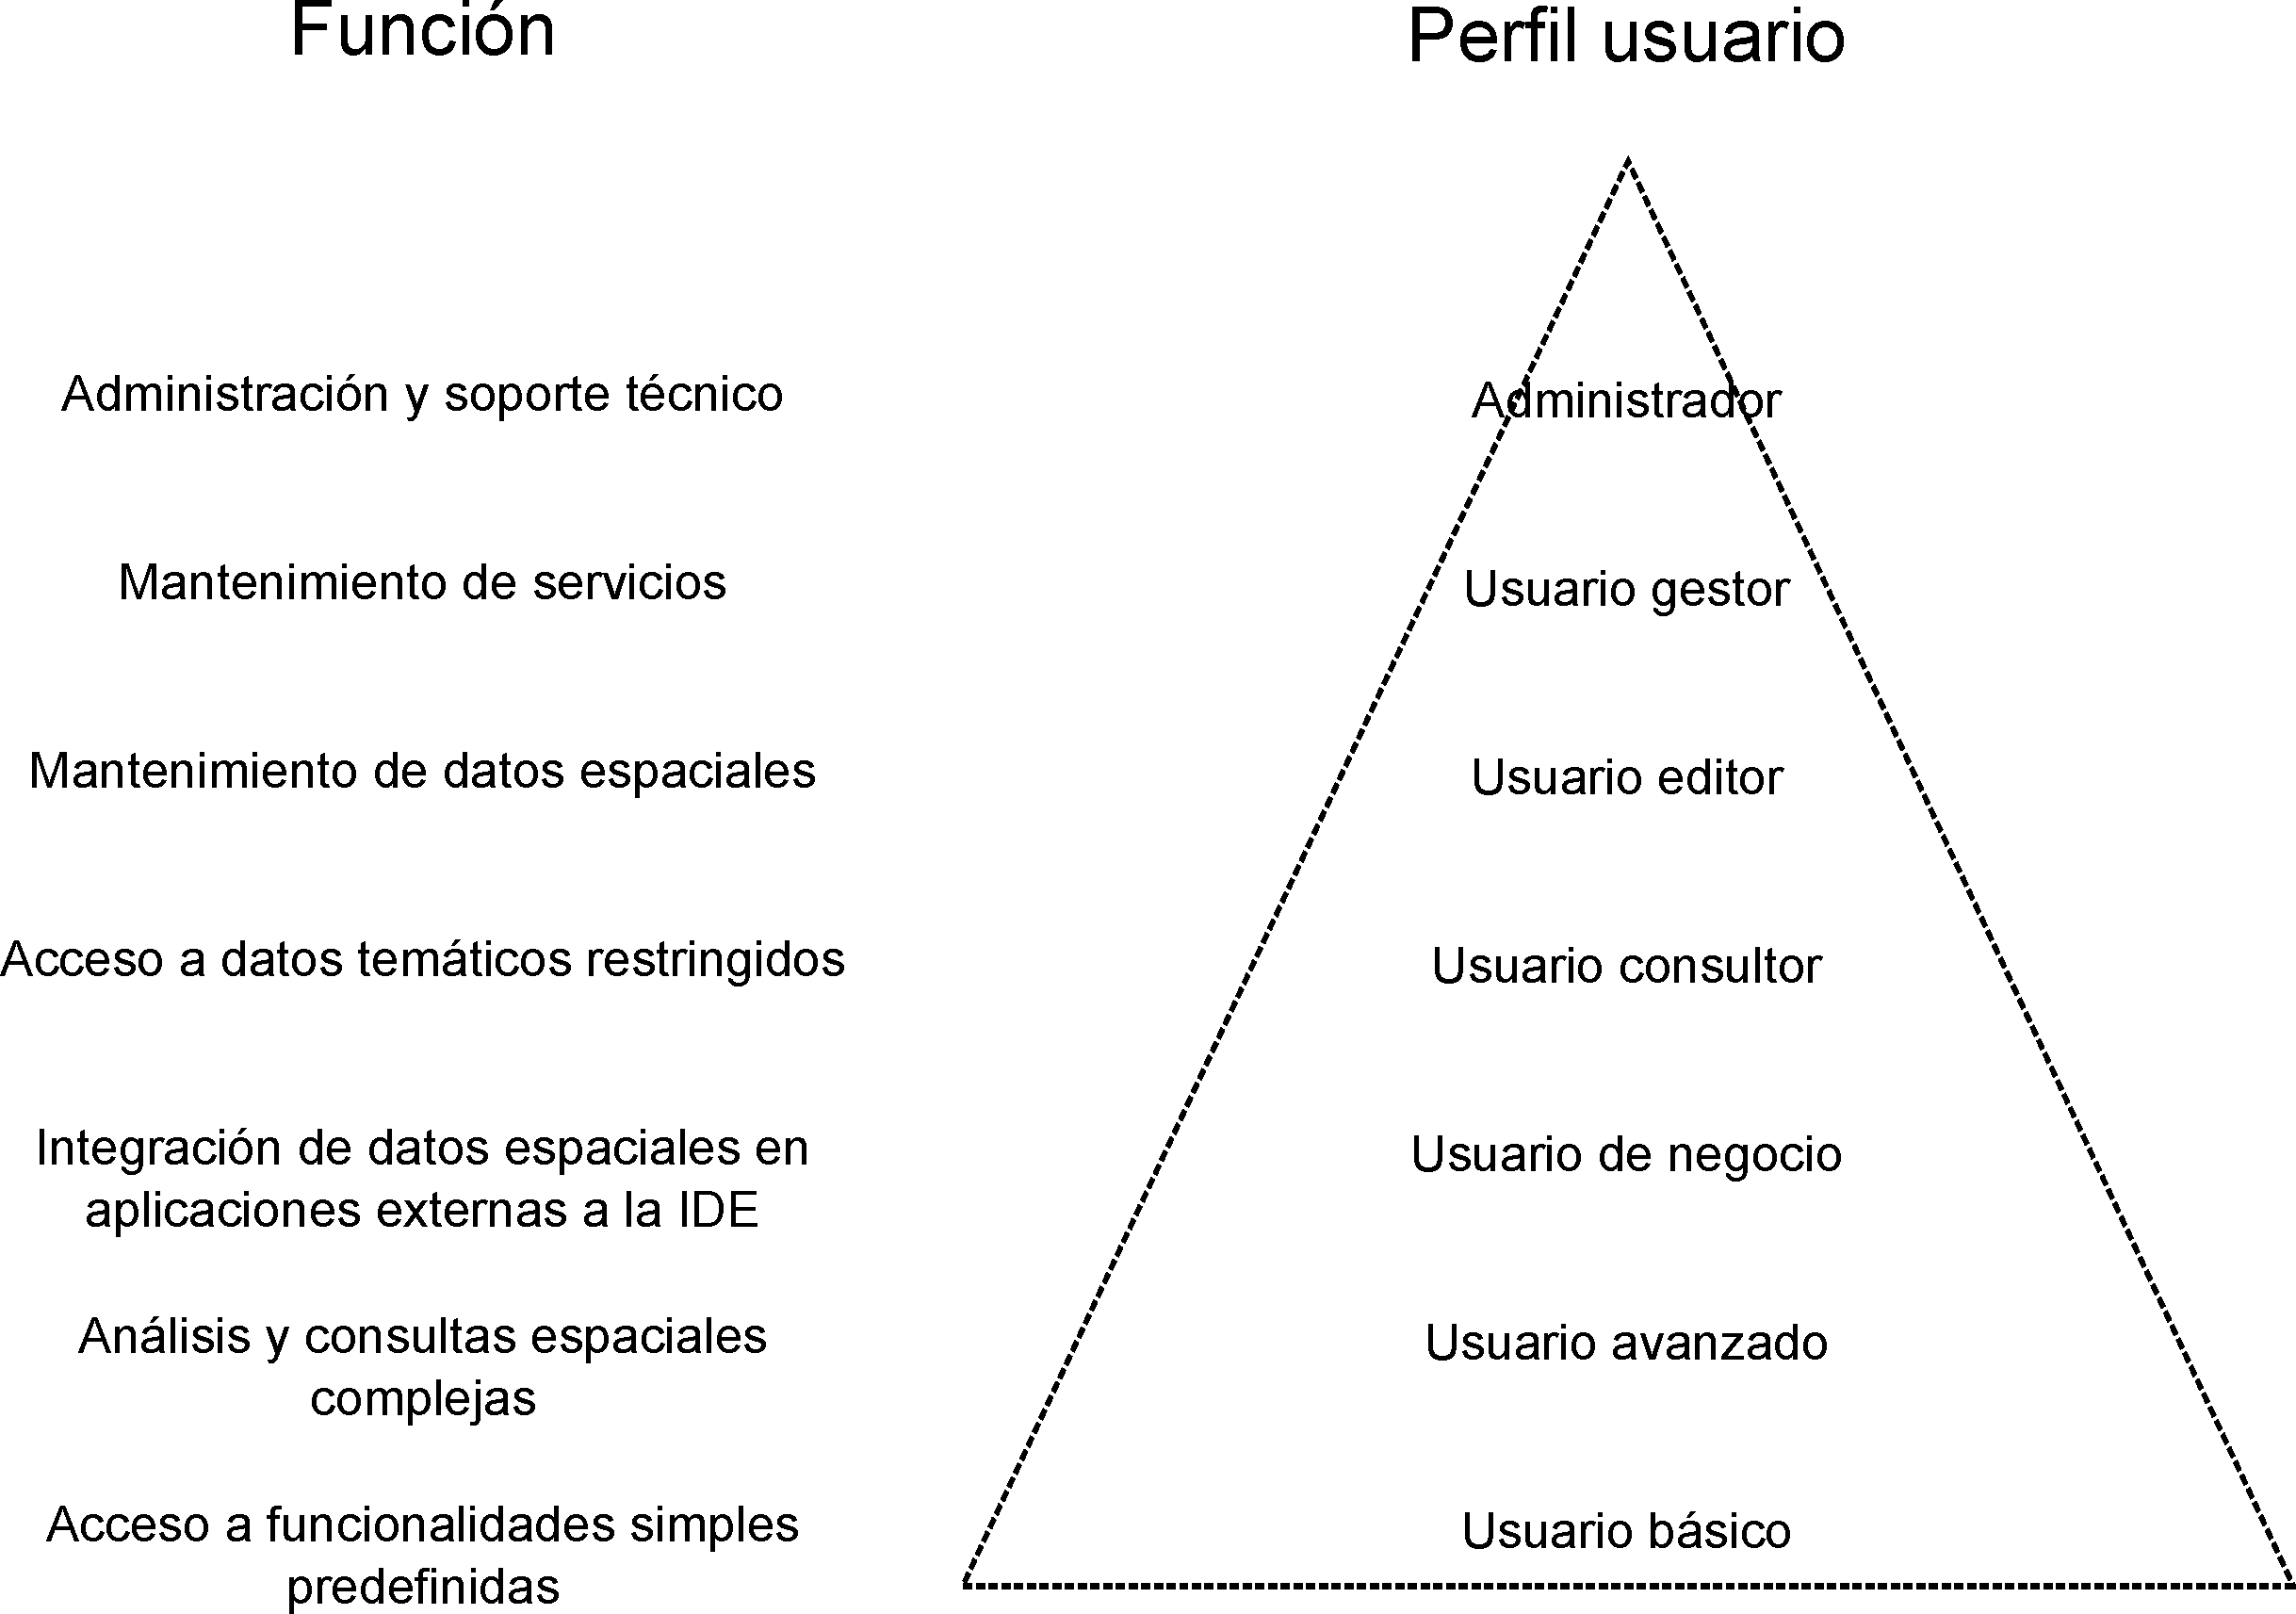
\includegraphics[width=.75\mycolumnwidth]{IDE/usuariosIDE.pdf}
	\caption{\small Clasificaci�n de usuarios de una IDE (seg�n \cite{Rodriguez2005JIDEE})}\label{Fig:UsuariosIDE} 
\end{figure}

Adem�s de los usuarios, otros actores involucrado en una IDE son los organismos internacionales de creaci�n de est�ndares, en concreto la organizaci�n de estandarizaci�n internacional ISO con sus miembros nacionales, el Open Geospatial Consortium (OGC) y el World Wide Web Consortium (W3C). Estos organismos definen las normas y est�ndares que formar�n la base tecnol�gica de la IDE y que permitir�n su interoperabilidad.

Junto a los anteriores, encontramos al responsable particular de cada nodo IDE. Este responsable puede ser una administraci�n p�blica, una empresa, una universidad, un centro tecnol�gico u otro tipo de organismo que se hace responsable de la administraci�n del nodo IDE y de establecer los est�ndares que se deben cumplir dentro de su �mbito, as� como normas o recomendaciones adicionales. A modo de ejemplo, para la IDE de Espa�a el responsable es el Instituto Geogr�fico Nacional, para la IDE de Galicia el responsable es el Sistema de Informaci�n Territorial de Galicia y para la IDE de la provincia de A Coru�a el responsable es la Diputaci�n de A Coru�a.

De entre todos los responsables que podemos encontrar en el conjunto de nodos de una IDE, las Agencias Cartogr�ficas Nacionales resultan especialmente relevantes, por las siguientes razones \cite{Kok2009}:

\begin{itemize}
	\item Son responsables de los registros cartogr�ficos en el dominio p�blico y desempe�an un papel fundamental en el desarrollo de las IDE. 
\item Son las instituciones que deben impulsar la puesta en marcha de est�ndares y establecer las bases que permitan el intercambio de informaci�n y la creaci�n de geoportales, as� como de los acuerdos jur�dicos e institucionales relacionados con las IDE. Ponen en marcha plataformas de car�cter p�blico junto con otros colaboradores de las IDE para estimular la implementaci�n de las IDE en los programas y procesos nacionales y de gobierno. \item Establecen los acuerdos institucionales para la regulaci�n de las IDE y juegan un papel de liderazgo en la toma de decisiones al nivel del gobierno central.
\item Juegan un papel important�simo enlazando la comunidad profesional con los responsables pol�ticos. 
\end{itemize}

Finalmente, consideramos tambi�n como actores al resto de nodos de la IDE, ya que se debe alcanzar la coherencia de la informaci�n evitando la duplicidad de esfuerzos.

\section{Algo m�s sobre cat�logos}

Los cat�logos son la parte visible de la IDE, ya que proporcionan la puerta de entrada a los datos de esta y est�n pensados para simplificar la labor de encontrar y obtener los datos necesarios para cada usuario. Otros elementos de las IDE como metadatos o est�ndares son tratados en cap�tulos independientes dentro de esta parte del libro. Sin llegar a requerir un cap�tulo espec�fico, los cat�logos no obstante son piezas imprescindibles sobre las que es necesario profundizar, por lo que en este apartado describiremos con algo m�s de profundidad su papel y sus caracter�sticas como partes clave de una IDE.

El cat�logo permite al usuario navegar de forma eficaz por la informaci�n contenida en una IDE, bien sea en uno de sus nodos de forma aislada o bien en el conjunto de la red de nodos que forman la IDE. Los nodos, como ya sabemos, deben estar conectados y relacionados, y es en virtud de esa conexi�n y gracias al uso de lenguajes comunes (est�ndares) que pueden comunicarse y compartir su informaci�n. De este modo, un cat�logo puede ofrecer los datos contenidos en el nodo en el que se encuentra, pero tambi�n <<preguntar>> a otros nodos y devolver al usuario una respuesta que tenga tambi�n en cuenta los datos de esos otros nodos. Como vimos en el cap�tulo \ref{Servidores_y_clientes_remotos}, esa respuesta a consultas es uno de los servicios que pueden ofrecerse basados en informaci�n geogr�fica.

El cat�logo dispone de una interfaz, que es la que el usuario emplea para plantear sus b�squedas y obtener respuestas. Esta interfaz se localiza normalmente en el \emph{portal} de acceso al cat�logo, y proveen el acceso m�s directo a los contenidos de la IDE. Estos contenidos no se limitan exclusivamente a los datos, ya que pueden incluir servicios de distintos tipos (recordemos que, seg�n vimos en el cap�tulo \ref{Servidores_y_clientes_remotos}, lo datos pueden servirse de varias formas), incluyendo servicios que no se basen directamente en los datos de la IDE, tales como procesos.\index{Portal}

En la figura \ref{Fig:Catalogo_UNEX} puede verse un ejemplo de una interfaz de acceso a un cat�logo.

\begin{figure}[!hbtp]   
	\centering
	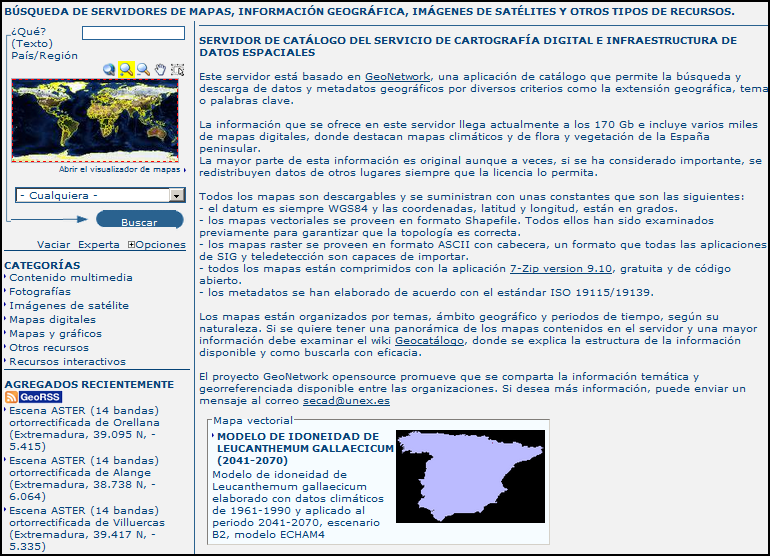
\includegraphics[width=0.85\textwidth]{IDE/CatalogoUNEX.png}
	\caption{\small Interfaz de acceso al cat�logo de la IDE de la Universidad de Extremadura}\label{Fig:Catalogo_UNEX} 
\end{figure}

Cuando nos referimos a un usuario del cat�logo, este no ha de ser necesariamente una persona, y no ha de <<ver>> la interfaz dispuesta para el acceso. El cat�logo puede ser consultado por, por ejemplo, otro ordenador, ya que expone sus capacidades como un servicio m�s, y eso es lo que permite que desde un nodo de la IDE se puedan realizar consultas sobre nodos distintos. La �nica condici�n para que esto suceda es que los nodos puedan entenderse entre s� en un lenguaje com�n. Para ello existen los est�ndares, que se han mencionado ya como parte de la IDE y que veremos m�s extensamente en el cap�tulo \ref{Estandares}. 

De otro modo, podemos entender al cat�logo como el bibliotecario que nos proporciona acceso a los documentos de una biblioteca. Es a �l a qui�n debemos dirigirnos para obtener uno de sus documentos, pero, en caso de que la biblioteca no disponga de lo que buscamos, puede llamar a otras bibliotecas y preguntar en ellas e incluso, si existen acuerdos de prestamo, facilitarnos la obtenci�n del documento sin necesidad de que tengamos que acudir personalmente a la biblioteca donde se encuentra. Puesto esto en el contexto de Internet y con informaci�n geogr�fica digital en lugar de documentos f�sicos, tenemos una descripci�n acertada del papel de los cat�logos como herramientas para el descubrimiento y obtenci�n de esa informaci�n.

Se suele emplear el t�rmino \emph{harvesting}\footnote{del ingl�s \emph{to harvest}: cosechar, recolectar} para indicar la capacidad de un nodo para recoger la informaci�n de otros y poder as� responder a peticiones teniendo en cuenta esa informaci�n ajena. Si los nodos soportan este tipo de operaciones, es posible sincronizar los metadatos entre ellos, de forma que cada nodo del cat�logo se enriquece con los restantes sin que ello suponga una carga extra de organizaci�n y mantenimiento de metadatos.

La figura \ref{Fig:UsuariosCatalogo} muestra un esquema de lo que la actividad de un usuario sobre un cat�logo supone en otros elementos de la IDE, y c�mo estos se relacionan a la hora de dar respuesta a su consulta.

\begin{figure}[!hbtp]   
	\centering
	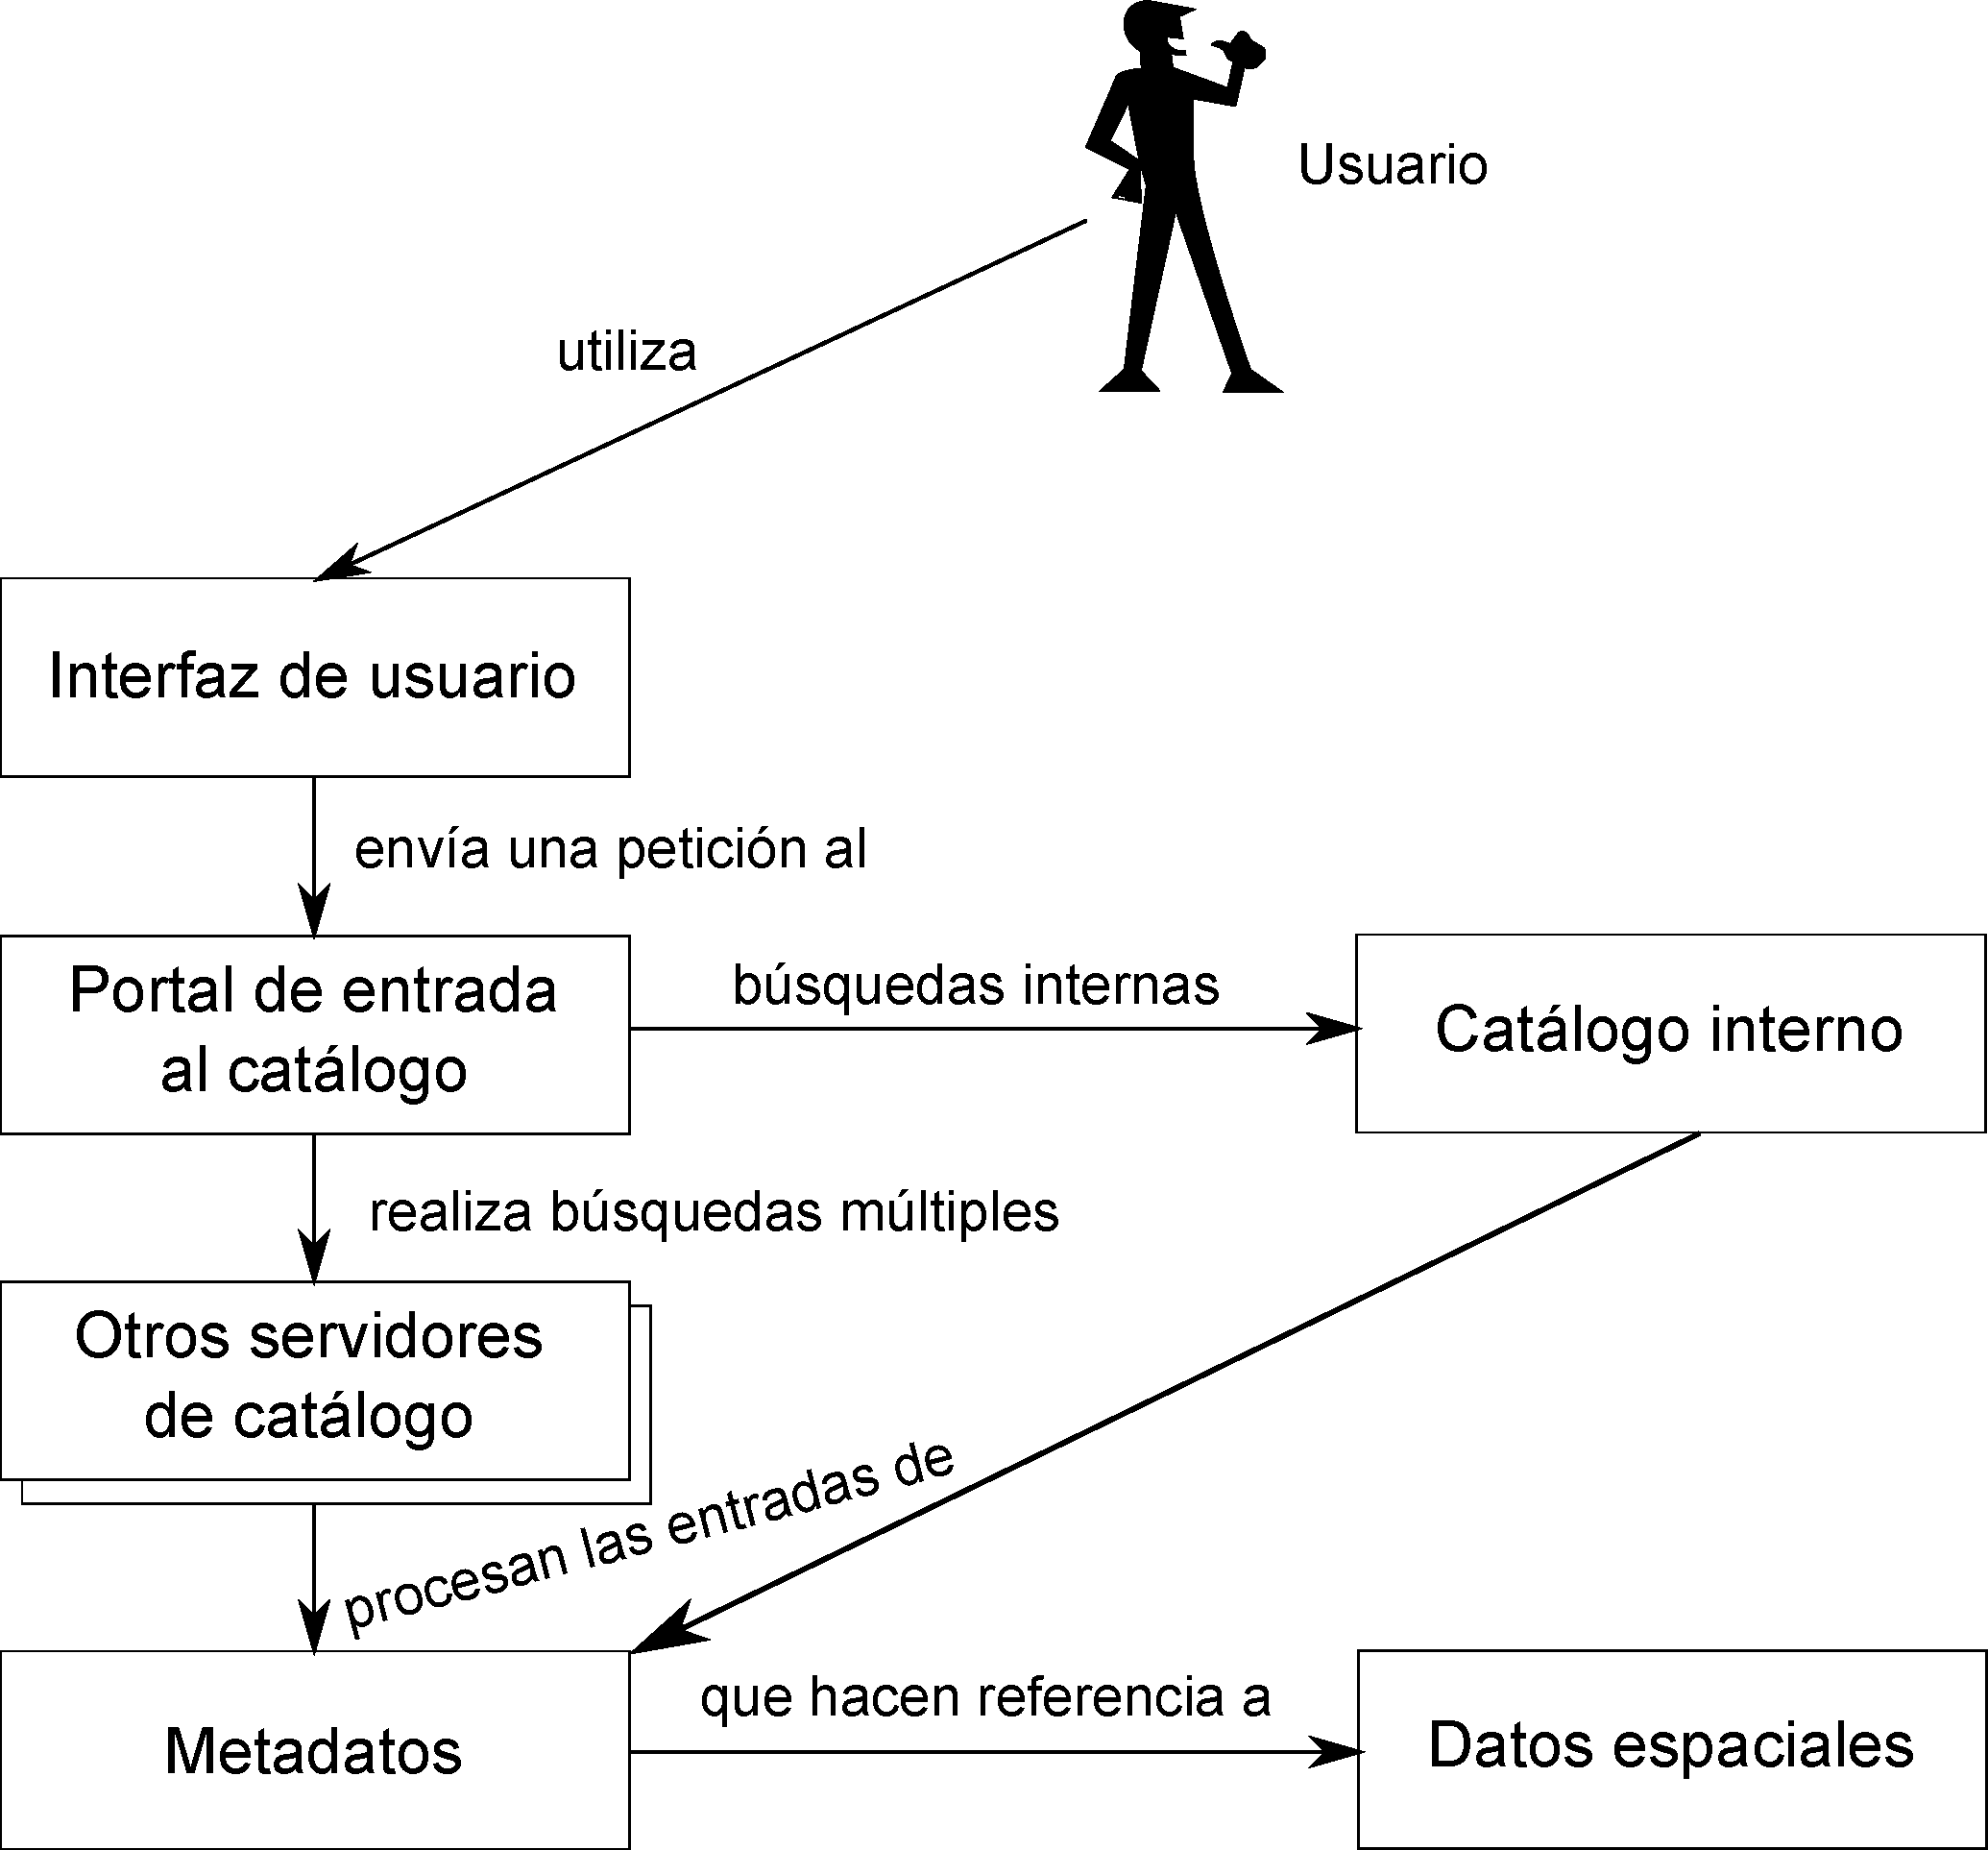
\includegraphics[width=0.5\mycolumnwidth]{IDE/usuariosCatalogo.pdf}
	\caption{\small Diagrama de interacci�n que muestra la utilizaci�n b�sica de servicios de cat�logo y los
elementos de IDE relacionados desde un punto de vista de un usuario (adaptado de \cite{RecetarioIDE})}\label{Fig:UsuariosCatalogo} 
\end{figure}

Viendo que los distintos nodos de una IDE est�n relacionados y bien comunicados, y que de igual modo lo han de estar sus cat�logos, un aspecto importante en relaci�n a estos �ltimos es, sin duda, la forma en que se relacionan. Cabe pensar que, si bien es necesario dividir todo el trabajo de gesti�n de datos de una IDE en una serie de nodos para repartir las tareas a distintas escalas y lograr una estructura �ptima, esto mismo no es estrictamente necesario en el caso de los cat�logos. Es decir, podr�an tenerse los datos divididos entre los distintos nodos, cada uno de los cuales permitiera el acceso a suyos datos mediante los correspondientes servicios, y tener un �nico cat�logo que contuviera todos los metadatos y un �nico portal de acceso a esos metadatos. Sin duda, esto facilitar�a el trabajo de buscar cualquier informaci�n geogr�fica, lo cual se har�a siempre a trav�s de un �nico portal. Sin embargo, tal centralizaci�n de actividades presenta muchas dificultades. Entre ellas, encontramos las siguientes:

\begin{itemize}
	\item Exceso de datos. Algunos nodos son muy voluminosos, con literalmente millones de elementos. Agrupar los metadatos correspondientes a todos ellos resultar�a en un volumen de datos excesivo, que colapsar�a el punto de entrada al cat�logo.
	\item Actualizaci�n m�s dif�cil. Los metadatos son din�micos, actualiz�ndose en muchos casos con gran frecuencia. Gestionar la actualizaci�n de todos ellos desde un nodo central no resulta pr�ctico, y complicar�a sumamente la labor de los encargados de mantener los metadatos.
\end{itemize}

A lo anterior hay que sumar las razones particulares que cada nodo puede tener para preferir encargarse �l mismo de la gesti�n de todos los elementos, incluido el cat�logo. Entre ellas podemos encontrar las ventajas que proporciona la independencia del nodo, pudiendo establecer sus propias regulaciones de acceso o enfocando el descubrimiento de datos de la forma que resulte m�s ventajosa al organismo responsable.

Aunque los nodos se comuniquen entre s� y puedan entenderse, no necesariamente deben compartir la informaci�n con un id�ntico nivel de detalle. Por ejemplo, para la descripci�n de sus datos a trav�s de metadatos, existen diversos est�ndares adaptados al tipo de dato geogr�fico de que se trate y al uso para el que este ha sido creado. Los nodos usar�n aquel que consideren m�s conveniente en cada caso. La existencia de un �nico cat�logo har�a imposible esa variabilidad, imponiendo una excesiva homogeneizaci�n que en la pr�ctica ser�a m�s perjudicial que beneficiosa.

Por lo anterior, el repositorio de datos y metadatos que forman parte de una IDE debe tener una naturaleza distribuida en todos sus elementos, siendo m�s ventajoso operar de ese modo desde la mayor�a de puntos de vista.

\section{Claves para el �xito}

La creaci�n exitosa de una IDE no depende �nicamente de disponer de los elementos que la forman y de establecer las relaciones entre elementos y actores. Al igual que en la implantaci�n de un SIG, existen circunstancias adicionales que deben considerarse para lograr que la IDE cumpla sus objetivos, y de las cuales depende su �xito. Por desgracia, no todos los intentos de creaci�n de una IDE que se han llevado a cabo desde la aparici�n de estas han sido igual de exitosos, y se han cosechado algunos fracasos notables. La experiencia de estos casos, junto con aquellos que s� han logrado plenamente sus objetivos, nos ense�a que las caracter�sticas m�s importantes que una IDE ha de reunir para poder funcionar exitosamente son los siguientes:

\begin{itemize}

\item La IDE debe estar preparada para responder a necesidades reales. Los usuarios solo acceder�n a los datos alojados en servidores si con esta informaci�n va a ser posible la realizaci�n normal de su trabajo. Esto implica tanto que los datos sean correctos como que la forma de acceso sea sencilla, r�pida y flexible.
\item La IDE debe ser homog�nea en su estructura a trav�s de los distintos niveles tanto a nivel tecnol�gico como a nivel sem�ntico.
\item Debe existir un responsable claro de la gesti�n de la IDE que debe encargarse de asegurar que est�n presentes los datos de referencia y que estos est�n actualizados y sean f�ciles de encontrar y de utilizar. Adem�s, debe estar claro qui�n es el responsable de capturar y mantener cada elemento de informaci�n.
\item La IDE debe estar respaldada por un presupuesto econ�mico y de personal suficiente que cubra las necesidades que vayan surgiendo.
\end{itemize}

Entre las razones principales a las que puede achacarse la implantaci�n poco exitosa de algunas IDE, la mayor�a pueden relacionarse con factores organizativos e institucionales. Otros factores, tales como los tecnol�gicos o los econ�micos, son causa igualmente de dificultades a la hora de establecer una IDE, aunque en menor medida. 

Algunas de las causas principales del fracaso de una IDE son las siguientes\cite{Morant2005JIDEE}:

\begin{itemize}
	\item La falta de cultura informacional.
	\item Las relaciones de poder.
	\item La falta de visiones globales y de objetivos comunes.
	\item Las actitudes o posturas de rechazo de las personas hacia las nuevas tecnolog�as.
	\item La falta de implicaci�n o inter�s por parte de los usuarios en el desarrollo y/o posterior uso de la IDE.
	\item La falta de coordinaci�n y liderazgo.
	\item La infravaloraci�n de los aspectos culturales y organizacionales.
	\item El desconocimiento del potencial de la informaci�n geogr�fica.
\end{itemize}

\section{Principales acuerdos e iniciativas}

La aparici�n del concepto de IDE ha tra�do consigo el desarrollo de numerosas iniciativas en los distintos niveles administrativos. Estas iniciativas han permitido que a d�a de hoy dispongamos de numerosas IDE operativas y funcionales, y son las que garantizan que cada una de ellas responda a los criterios establecidos y lo siga haciendo en el futuro. Cada Infraestructura de Datos Espaciales responde a una serie de elementos legislativos y pol�ticos, y es por ello que por cada nodo de una IDE debe existir un marco correspondiente, bien sea este particularizado para el nodo en cuesti�n o bien heredando los contenidos del aplicable al nodo de orden superior.

Aunque todav�a queda por hacer hasta llegar a un verdadero estado de madurez de las IDE a nivel mundial, el desarrollo que estas han sufrido durante los �ltimos a�os es muy notable, y el n�mero de IDE y de acuerdos que las sustentan es muy elevado. L�gicamente, no resulta de inter�s describir aqu� todas estas iniciativas, m�xime considerando que muchas de ellas tienen car�cter local y no tienen apenas relevancia en el �mbito global de las IDE. No obstante, s� que es relevante conocer las iniciativas pioneras en este sentido, as� como, especialmente,	algunos de los acuerdos existente en los niveles superiores. Saber acerca de ellos es necesario para comprender el panorama actual de las IDE y estar familiarizado con las propuestas que rigen la gran mayor�a de ellas. Veremos igualmente algunos ejemplos de acuerdos existentes en cada uno de los distintos niveles, para comprender las diferencias entre ellos y la conexi�n que a su vez existe.

En conjunto, estas iniciativas nos servir�n para detectar patrones comunes a todas ellas, ayud�ndonos a entender las caracter�sticas b�sica de las IDE a trav�s de algunos de sus representantes m�s importantes.

\subsection{GSDI}

La GSDI (Global Spatial Data Infrastructure) Association en una organizaci�n que agrupa a otras organizaciones, agencias, compa��as e individuos de todo el mundo con objeto de apoyar las IDE y su desarrollo con car�cter global. GSDI es responsable de aglutinar a todas ellas y coordinarlas, en un intento de trabajar en el nivel superior de la jerarqu�a de las IDE y poner en marcha una iniciativa que cubra la totalidad del territorio mundial.

GSDI se fund� en 1996, y viene hasta la fecha realizando un trabajo fundamentalmente basado en guiar el desarrollo de iniciativas locales y nacionales a�n en sus inicios o que todav�a no han llegado a comenzarse. En este sentido, GSDI act�a como un canalizador de toda la experiencia acumulada a lo largo de los �ltimos a�os por las distintas iniciativas IDE que han surgido, tratando de replicar en las IDE que empiezan a desarrollarse el buen hacer de las m�s exitosas, as� como evitar que se vuelvan a cometer los errores de las que no lo han sido tanto.

En sus propias palabras, la misi�n de la GSDI se puede resumir en los siguientes puntos.

\begin{itemize}
	\item Servir como punto de contacto para todos aquellos dentro de la comunidad global implicados en el desarrollo, implementaci�n y avance de los conceptos de las IDE
	\item Impulsar las IDE que apoyan sistemas sociales, econ�micos y medioambientales sostenibles, integrados desde la escala local a la global.
	\item Promover el uso informado y responsable de la informaci�n geogr�fica y las tecnolog�as espaciales para el beneficio de la sociedad.
\end{itemize}

\subsection{NSDI}

Aunque hoy en d�a pr�cticamente todos los pa�ses tienen su propia IDE, la IDE de los Estados Unidos es especialmente importante entre todas ellas, ya que fue la primera en aparecer. Es decir, Estados Unidos fue el primer pa�s en poner en marcha una iniciativa de gran calibre para apoyar a nivel nacional la creaci�n y manejo coordinados de informaci�n geogr�fica, tal como los principios fundamentales de un IDE establecen. Por ello, resulta especialmente ilustrativa, tanto por el �xito del proyecto en estos a�os y la influencia directa que en la actividades de otros pa�ses ha tenido, como por el car�cter de referente y la gran experiencia acumulada durante toda su existencia.

La Infraestructura de Datos Espaciales de Estados Unidos, denominada NSDI (National Spatial Data Infrastructure), surge en abril de 1994 como consecuencia de la promulgaci�n de la  Orden Ejecutiva 12906\cite{Clinton1994FR}, que insta a avanzar en la construcci�n de una infraestructura nacional de datos espaciales coordinada entre las administraciones federal, estatal y local, el sector privado y el acad�mico. Esta Orden recoge las propuestas redactadas un a�o antes por el Comit� Federal de Datos Geogr�ficos (FGDC) \cite{FGDC1993}, el cual queda a su vez como responsable del avance de la NSDI en el �mbito federal.

No resulta extra�o que la primera IDE apareciera en Estados Unidos, ya que el pa�s contaba con una larga trayectoria de otras propuestas similares que trataban de promover un manejo racional y eficiente de la informaci�n geogr�fica, dirigiendo a los organismos federales en la direcci�n adecuada para lograr esto. Asimismo, exist�a una importante tradici�n en el uso de las tecnolog�as de la informaci�n espacial, que desde sus primeros momentos hab�an contado con abundante apoyo por parte de la administraci�n.

El gobierno federal llevaba desde los a�os 50 tratando de concienciar sobre la importancia de coordinar las labores relativas a la informaci�n geogr�fica. De especial importancia resulta la Circular A--16, redactada en 1953 y posteriormente revisada en 1973 y 1990. En esta �ltima revisi�n se adaptan los contenidos a la nueva realidad de la informaci�n geogr�fica, en un contexto sensiblemente modificado gracias a la aparici�n de los SIG y la cartograf�a digital, lo cual inicia el camino hacia la aparici�n de las IDE, y en particular de la NSDI estadounidense. Fue igualmente en ese a�o, 1990, cuando se creo el FGDC, en el cual se encuentran representadas las principales agencias federales con competencias en la producci�n de informaci�n espacial, y tambi�n, recientemente, otros organismos de  de la administraci�n estatal y local, as� como del sector acad�mico y privado.

Seis son los objetivos principales que se plantean en la NSDI, a saber \cite{Echeverria2001Boletic}:

\begin{enumerate}
	\item La implantaci�n de mecanismos para el descubrimiento, acceso y distribuci�n de datos, materializados en una red electr�nica distribuida que enlace a productores, gestores y usuarios de informaci�n geogr�fica. 
\item El establecimiento de est�ndares de intercambio de informaci�n. 
\item La documentaci�n de los conjuntos de datos espaciales existentes y producidos en el futuro de acuerdo a un est�ndar de metadatos y su difusi�n p�blica a trav�s de la red.
\item La identificaci�n y desarrollo de los conjuntos de datos espaciales m�s comunes y habitualmente necesitados (lo que se conoce como \emph{framework} o \emph{datos marco}).
\item La difusi�n p�blica de la informaci�n espacial producida por la administraci�n federal.
\item El establecimiento de acuerdos entre organismos para la producci�n de informaci�n espacial de inter�s conjunto, de forma que se eviten duplicidades y solapes de esfuerzos.
\end{enumerate}

Desde la creaci�n de la NSDI, se ha avanzado notablemente en estos puntos, pudiendo decirse que se trata de una iniciativa exitosa que a lo largo de estos a�os ha logrado una buena parte de sus objetivos. El trabajo desarrollado ha tenido adem�s una gran influencia en el �mbito de las IDE por su car�cter pionero, lo que convierte a la NSDI en un referente de primera l�nea dentro de este campo.


\subsection{INSPIRE}

INSPIRE \cite{inspire07} es la principal directiva europea relativa a informaci�n geogr�fica, y surge como continuaci�n de algunos intentos previos que llevaban desarroll�ndose en Europa desde los a�os 90, todos ellos sin demasiado �xito. El problema de estas propuestas era que no part�an de alg�n �rgano de gobierno comunitario, sino directamente de los productores de cartograf�a.

En septiembre de 2001, sin embargo, surge una iniciativa de la Direcci�n General de Medio Ambiente de la Uni�n Europea, encaminada tambi�n a mejorar el manejo de informaci�n geogr�fica en sus tareas y proyectos, gran parte de los cuales son de car�cter transfronterizo.

En conjunto con la Agencia Europea Eurostat, y el Instituto para el Medio Ambiente y la Sostenibilidad, a trav�s de su Centro de Investigaci�n Com�n (Joint Research Center, JRC), ponen en marcha la iniciativa INSPIRE (Infraestructure for Spatial Information in Europe), cuyos objetivos principales son \cite{Inspire2005IGN}:

\begin{itemize}
	\item Poner a disposici�n de �rganos responsables de toma de decisiones o aplicaci�n de pol�ticas comunitarias (esencialmente de Medio Ambiente) datos espaciales abundantes y fiables.
\item Establecer servicios integrados de Informaci�n Geogr�fica (IG), basados en una red distribuida de bases de datos, enlazadas por normas comunes y protocolos que aseguren la interoperabilidad.
\item Optimizar los datos disponibles mediante la documentaci�n de la informaci�n espacial.
\item Lograr la coherencia de la informaci�n espacial entre diferentes niveles y temas.
\item Crear servicios destinados a mejorar la accesibilidad e interoperabilidad de los datos y a la eliminaci�n de obst�culos para su utilizaci�n.
\end{itemize}

A finales de 2001, se constituye un grupo de expertos formado por representantes de los Estados Miembro, de los pa�ses candidatos, as� como representantes regionales y de los principales organismos directamente vinculados con la producci�n y explotaci�n de informaci�n tanto medioambiental como geogr�fica.

Este grupo de expertos da forma a unos principios que han de regir el desarrollo de INSPIRE, y que son los siguientes\cite{Ryttersgaard2004FIG}:

\begin{itemize}
	\item Los datos deber recogerse y mantenerse en el nivel en el que esto resulte m�s efectivo.
	\item Debe ser posible combinar de modo continua informaci�n geogr�fico de distintas fuentes a lo largo de toda Europa y compartirla entre m�ltiples usuarios y �mbitos de aplicaci�n.
\item Debe ser posible que la informaci�n recogida en un nivel se comparta con otros niveles.
\item La informaci�n geogr�fica necesaria para una correcta gesti�n debe ser abundante bajo condiciones que no impidan su uso extensivo.
\item Debe ser f�cil descubrir qu� informaci�n geogr�fica est� disponible, re�ne las caracter�sticas para un uso determinado y bajo qu� condiciones puede ser obtenida y usada.
\item Los datos geogr�ficos deben ser sencillos de entender e interpretar, as� como de seleccionarse en un entorno de usuario amigable.
\end{itemize}

Desde la redacci�n de estos principios, INSPIRE ha seguido su desarrollo hasta finalmente ser aprobada de modo formal por el Consejo Europeo (29 de enero de 2007) y el Parlamento Europeo (12 de febrero de 2007). Fue publicada como Directiva 2007/2/CE el 14 de marzo de 2007.

La figura \ref{Fig:EvolucionINSPIRE} muestra un esquema de la secuencia temporal que ha seguido INSPIRE, desde su nacimiento hasta la actualidad.

\begin{figure}[!hbtp]   
	\centering
	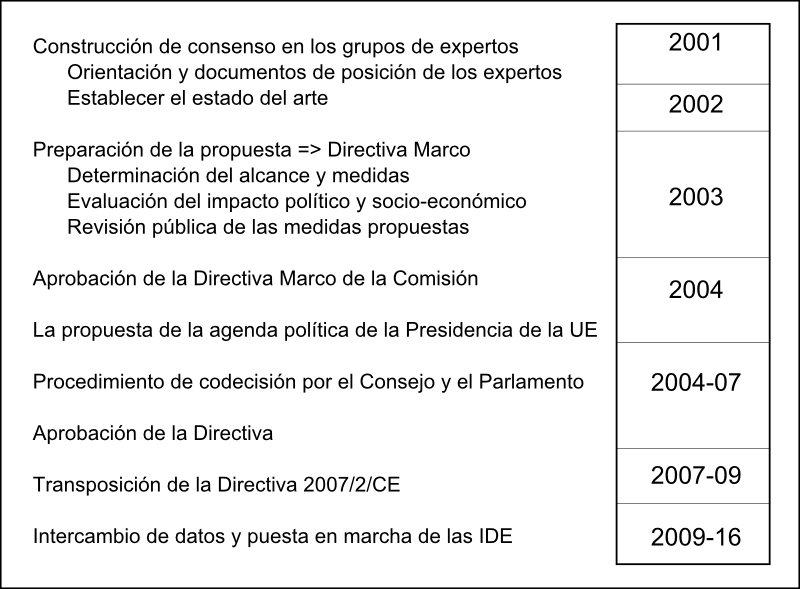
\includegraphics[width=0.65\mycolumnwidth]{IDE/EvolucionINSPIRE.pdf}
	\caption{\small Secuencia temporal seguida por INSPIRE (adaptado de \cite{Craglia2009INSPIRE})}\label{Fig:EvolucionINSPIRE} 
\end{figure}

INSPIRE contiene 3 anexos en los que se especifica qu� datos deben formar parte de la IDE, ya sea con car�cter obligatorio o con car�cter opcional. De este modo, se establece el contenido deseado para los datos creados y almacenados por los distintos nodos de la IDE, con objeto de obtener un conjunto global de datos coherente y facilitar la realizaci�n de la mayor parte de tareas en todos los lugares, as� como a todos los niveles de detalle. Es decir, que exista una coherencia tanto horizontal como vertical en lo que a datos existentes respecta.

Las tablas en \ref{Tabla:INSPIREAnexos} muestran los tipos de datos que se recogen en los citados anexos.

\begin{table*}[!hbt]
\centering 

\begin{tabular}{cp{1cm}c}
\begin{tabular}{c} \toprule
\textsf{Anexo I: Datos de referencia} \\ \midrule
Sistema de ref. de coordenadas\\
Cuadr�culas geogr�ficas\\
Nombres geogr�ficos\\
Unidades administrativas\\
Redes de transporte\\
Hidrograf�a\\
Lugares protegidos \\ \bottomrule
\end{tabular}

& &

\begin{tabular}{c} \toprule
\textsf{Anexo I: Datos de referencia}  \\ \midrule
Modelos de Elevaciones\\
Direcciones y �reas postales\\
Parcelas catastrales\\
Ocupaci�n del suelo\\
Ortofotos \\ \bottomrule
\end{tabular}
\end{tabular}

\vspace{0.5cm}

\begin{tabular}{c|c} \toprule
\multicolumn{2}{c}{\textsf{Anexo III: Datos tem�ticos}}  \\ \midrule
Unidades estad�sticas & Edificaciones\\
Edafolog�a & Geolog�a \\
Uso del suelo & Salud y seguridad humana\\
Instalaciones de servicios & Instalaciones industriales y productivas\\
Instalaciones Agr�colas y Acuicultura & H�bitats y biotopos \\
Regiones biogeogr�ficas & Demograf�a y distribuci�n de la poblaci�n\\
�reas restringidas o reguladas & Zonas de riesgos naturales \\
Condiciones Atmosf�ricas & Caracter�sticas meteorol�gicas \\
Caracter�sticas oceanogr�ficas & Regiones Marinas\\
\bottomrule
\end{tabular}

\caption{\small Datos especificados por los anexos I, II y III de INSPIRE, estableciendo los datos de referencia y tem�ticos a incluir en una IDE.}
\label{Tabla:INSPIREAnexos}
\end{table*}


\subsection{Las IDE en Espa�a}

Adem�s de las iniciativas anteriores, existen en el mundo muchas otras de menor escala o m�s recientes, muchas de las cuales todav�a no est�n plenamente establecidas, y cuyo �xito no puede a�n garantizarse dada su corta vida. 

En lo que a Espa�a respecta, contamos con la Infraestructura de Datos Espaciales Espa�ola (IDEE) \cite{webIDEE}, que se encarga de coordinar a las distintas organizaciones del �mbito nacional implicadas en la producci�n y distribuci�n de cartograf�a. La IDEE arranc� en 2002 cuando la Comisi�n Permanente del Consejo Superior Geogr�fico aprob� el 10 abril la puesta en marcha de una Infraestructura Nacional de Datos Espaciales. En noviembre de ese mismo a�o se estableci� un Grupo de Trabajo IDEE con todos los actores implicados. El grupo se organiz� a su vez cuatro Subgrupos de Trabajo: Datos de Referencia, Metadatos, Arquitectura y Normas, y Pol�tica de Datos, Precios y Licencias. En la actualidad el n�mero de estos subgrupos es de 11.

Previamente a la reuni�n de este Grupo de Trabajo, exist�an proyectos anteriores cuya labor y experiencia se integra en la IDEE en la medida de lo posible. Uno de los m�s destacados es DIGA, un proyecto propio de metadatos coordinado por el Instituto Geogr�fico Nacional, en funcionamiento desde 1997.

Cuatro son las acciones propuestas para establecer la IDEE \cite{Rodriguez2003Mapping}:

\begin{enumerate}
	\item Creaci�n de un Portal Nacional de la IDE Espa�ola, que sirva de punto de entrada gen�rico para Espa�a y cumpla la funci�n de paraguas que acoja todos los recursos disponibles que la configuran.
	\item Establecimiento de un Nodo Espa�ol de Datos de Referencia (Topogr�ficos), que acoja en la IDE todos aquellos datos que pueden ser considerados de referencia en el sentido definido por INSPIRE.
	Otros nodos espa�oles tem�ticos o sectoriales (Datos Ambientales, Geol�gicos, Inventario Forestal...) estar�n accesibles en horizontal desde el mencionado Portal Nacional y convivir�n al mismo nivel con el Nodo Espa�ol de Datos de Referencia (Topogr�ficos).
	\item Implementaci�n de un Cat�logo que permita consultar de modo transparente e interoperable los metadatos que describen los distintos conjuntos de datos de referencia almacenados y documentados en sus respectivos centros de producci�n (IGN, ICC, ICA, DG del Catastro, etc.).
	\item Implementaci�n de un conjunto de servicios que permita al usuario final solicitar servicios de geoprocesamiento, sencillos en un primer momento, que pueden evolucionar a otros m�s complejos.
	\item Armonizaci�n gradual y progresiva de los recursos y componentes integrados en la IDE.
\end{enumerate}

Estando situada dentro del �mbito cubierto por INSPIRE, la IDEE debe cumplir lo establecido por esta directiva, manteniendo siempre sus caracter�sticas dentro de las recomendaciones, aunque pudiendo a�adir sus propios elementos.

Por debajo de la IDEE existen numerosas IDE regionales, las cuales proveen una buena parte de la informaci�n sobre la que se sustenta esta primera. Puede decirse que las IDE regionales gozan de buena salud, existiendo algunas de ellas desde el mismo momento en que la IDEE hizo su aparici�n. Uno de los proyectos pioneros a nivel regional en Espa�a es la IDE de Catalu�a. En \cite{Craglia2010IJSDIR} puede encontrarse un interesante estudio sobre IDE regionales, su viabilidad y �xito, basado en las IDE de Catalu�a y de la regi�n de Lombard�a.

La importancia de las IDE regionales no debe subestimarse, ya que sin ellas el funcionamiento de la IDE a otros niveles resultar�a pr�cticamente imposible. 

\begin{figure}[!hbtp]   
	\centering
	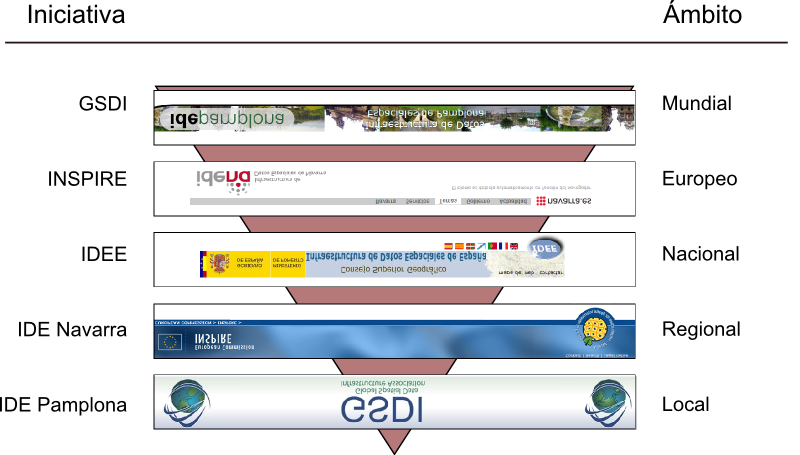
\includegraphics[width=0.85\textwidth]{IDE/EjemploIDE.pdf}
	\caption{\small Ejemplo de estructura a distintos niveles para una IDE particular (IDE de Pamplona) (adaptado de \cite{Echeverria2001Boletic})}\label{Fig:EjemploIDE} 
\end{figure}

Como cierre de este apartado, en la figura \ref{Fig:EjemploIDE} puede verse un ejemplo de iniciativas a distintos niveles y la jerarqu�a existente entre ellas. Obs�rvese c�mo se relacionan algunas de las iniciativas presentadas en los apartados anteriores, y la dependencia existente.


\section{Resumen}

La situaci�n actual en lo referente a la informaci�n geogr�fica	hace necesario promover una correcta coordinaci�n entre todos los organismos productores de datos espaciales, desde el nivel local al nivel estatal, con objeto de facilitar la explotaci�n de esa informaci�n y evitar esfuerzos redundantes. Con este objetivo, surgen a partir de la mitad de la d�cada de los 90 las Infraestructuras de Datos Espaciales, las cuales se componen de un conjunto de datos espaciales, tecnolog�a, normas y planes institucionales.

Existen diferentes niveles en una IDE, as� como diferentes actores implicados, haciendo que una IDE sea mucho m�s que un conjunto de datos espaciales. Algunos de los elementos principales de una IDE son los metadatos, los est�ndares (veremos m�s sobre estos dos elementos en pr�ximos cap�tulos) y los cat�logos. Estos �ltimos permiten el descubrimiento de informaci�n geogr�fica y son el punto de entrada a los contenidos de las IDE. Las IDE se organizan mediante un conjunto de nodos, los cuales est�n a su vez interconectados y coordinados.

Estados Unidos fue pionera en el establecimiento de una IDE, aunque actualmente existen iniciativas en la mayor�a de pa�ses. En la Uni�n Europea, la directiva INSPIRE dicta las pautas para el establecimiento de IDE en los pa�ses miembro, que han de crear sus propias IDE siguiendo los preceptos establecidos en ella.
% 

\chapter{Metadatos}\label{Metadatos}

\chapterauthor{Blake, Landon; Olaya, V�ctor}

\begin{keypoints}
�Qu� son los metadatos? $\bullet$ �Cu�l es su funci�n? $\bullet$ �C�mo se crean metadatos para la informaci�n geogr�fica? $\bullet$ �Qu� informaci�n contienen los metadatos? $\bullet$
\end{keypoints}

\bigskip

\begin{intro}
Los metadatos son aquellos datos que describen los datos espaciales y los servicios disponibles en una IDE. Los metadatos son uno de los puntos de entrada a la informaci�n geogr�fica contenida en una IDE ya que permiten a un actor sin ning�n conocimiento de esta consultar qu� puede ofrecer. En este cap�tulo describiremos en detalle qu� son los metadatos, su utilidad, y c�mo crearlos y emplearlos.
\end{intro}

\section{Introducci�n}

Los datos contienen la informaci�n geogr�fica, y es esta la que empleamos en un SIG para realizar las distintas operaciones que ya hemos visto en anteriores cap�tulos de este libro. No obstante, esos datos pueden resultar insuficientes, ya que el proceso de interpretaci�n mediante el que extraemos la informaci�n a partir de estos puede requerir conocer alguna otra serie de elementos.

Por ejemplo, si tenemos las coordenadas de un punto disponemos de un dato, pero para interpretarlo correctamente necesitamos conocer, entre otras cosas, el sistema de coordenadas en que vienen expresadas esas coordenadas. El dato con el que trabajamos (las coordenadas), requiere unos datos adicionales (por ejemplo, el c�digo EPSG del sistema de referencia empleado) para cobrar verdadero sentido.

Surge as� el concepto de \emph{metadatos}. Literalmente, los metadatos son <<datos acerca de los datos>> y su misi�n es \emph{explicar} el significado de los datos. Es decir, ayudan a los usuarios de los datos a entender mejor el significado que estos tienen y la informaci�n que guardan. Los metadatos son un documento adicional que acompa�a a los datos, y que permite una mejor gesti�n y una utilizaci�n m�s precisa de ellos.

Trabajando en el entorno de un SIG, los datos con los que trabajamos son de tipo espacial, y como ya estudiamos en su momento (v�ase el apartado \ref{ComponenteInformacionGeografica}), existe una componente espacial y una tem�tica. Los metadatos pueden referirse a ambas componentes, ya que es necesario documentar todas ellas, y podemos encontrar metadatos referidos a una capa de forma global, a su componente espacial o a su componente tem�tica.

Un ejemplo de metadato global de una capa puede ser el nombre de su autor o la fecha en la que ese dato ha sido creado. El sistema de referencia en el que se expresan las coordenadas de cada entidad recogida es un tipo de metadato relativo a la componente espacial. Y en lo referente a la componente tem�tica, los metadatos pueden recoger las unidades en las que se recoge una variable asociada a cada entidad, o bien almacenar cualquier otro valor que permita una mejor interpretaci�n de esa variable.

En una definici�n m�s formal, los metadatos son archivos de informaci�n que recogen las caracter�sticas b�sicas de alg�n dato o recurso. Representan el qui�n, qu�, cu�ndo, d�nde, c�mo y por qu� de ese recurso. Los metadatos geoespaciales se emplean para documentar recursos geogr�ficos digitales tales como una base de datos espacial, un SIG o una imagen de sat�lite. Un registro de metadatos incluye elementos b�sicos tales como el t�tulo o nombre del recurso, elementos geogr�ficos como la extensi�n que cubre el dato o el sistema de coordenadas empleado, as� como elementos relativos a la base de datos asociada tales como la definici�n de cada uno de sus campos o el dominio en que se encuentran los valores de estos \cite{webFGDC}.

El concepto de metadato no es algo nuevo y exclusivo de los datos digitales, ya que un mapa impreso tambi�n contiene metadatos en cierta forma. Una leyenda o un texto en un margen del mapa con informaci�n sobre la fecha en que se ha creado son tambi�n metadatos. En el caso de los datos geogr�ficos digitales, los metadatos no forman parte del dato directamente sino que son independientes de este. Ello permitir� realizar operaciones separadamente con los metadatos, tales como b�squedas, que abren nuevas posibilidades y dan un gran valor a estos.

\section{La utilidad de los metadatos}

Dependiendo del tipo de dato con el que trabajemos y las operaciones que deseemos realizar con ellos, los metadatos correspondientes ser�n m�s o menos necesarios, pudiendo ser pr�cticamente irrelevantes o bien completamente imprescindibles. Por ejemplo, si se trabaja con una �nica capa y gran parte de la informaci�n que esta contiene no va a emplearse para la realizaci�n de operaciones, los metadatos son menos necesarios que si se da un uso m�s intenso a los datos. 

En algunos casos, incluso si carecemos de metadatos, resulta posible interpretar correctamente los datos, como sucede si trabajamos con un MDE y valores de elevaci�n en metros. Es f�cil saber que los valores de elevaci�n se encuentran en esas unidades aplicando cierta l�gica, y procesarlos correspondientemente aunque no exista un dato explicito que as� nos los indique. 

En otras circunstancias, los metadatos son necesarios, pues contienen informaci�n que no puede inferirse directamente desde los propios datos. Si varias capas est�n en sistemas de coordenadas distintos y deseamos aplicar las transformaciones correspondientes para unificarlos en uno �nico y procesarlas de manera conjunta, estas transformaciones no se pueden llevar a cabo si no conocemos el sistema de origen del que partimos en cada capa. En este supuesto, el trabajo con los datos viene condicionado a que existan los metadatos correspondientes.

Los metadatos son, por tanto, sumamente importantes en el trabajo con SIG y, como veremos en breve, cobran una importancia mayor todav�a cuando no nos encontramos en el contexto de un uso aislado de los datos, sino cuando nos situamos en un entorno de un gran volumen de datos y numerosos usuarios. 

Dos de las funciones principales de los metadatos son garantizar el uso correcto y adecuado de los datos y facilitar su gesti�n, localizaci�n y consulta.

\subsection{Garantizar el uso correcto de los datos}

Uno de los beneficios m�s importantes que proporcionan los metadatos es asegurar que los datos espaciales son empleados de forma adecuada. Los datos espaciales, como muchos otros datos, son creados habitualmente para un determinado objetivo, y este objetivo no ha de ser necesariamente evidente o contenerse como tal en los datos mismos. Cuando se emplean esos datos para un objetivo distinto a aquel para el que fueron dise�ados, pueden surgir problemas debido a que se est� realizando un proceso para el que los datos con los que se trabaja presentan carencias. A continuaci�n veremos algunos ejemplos para ilustrar algunas situaciones en las que puede producirse un uso indebido de los datos, las cuales podr�an corregirse o evitarse mediante el empleo de los correspondientes metadatos.

\begin{itemize}
\item Ejemplo 1: Un organismo crea un juego de datos con los ejes de las principales v�as de una ciudad. Estos datos se emplean para labores de mantenimiento, de tal modo que faciliten la localizaci�n de las se�ales viales en la realizaci�n de inventarios. El juego de datos no contiene informacion sobre direcciones ni tampoco almacena la topolog�a de la red. Posteriormente, una compa��a especializada en reparto adquiere estos datos para el c�lculo de rutas �ptimas desde sus almacenes hasta las direcciones de destino de sus clientes.

\item Ejemplo 2: Un organismo crea un juego de datos con los elementos de la red de alcantarillado tales como alcantarillas, tuber�as, bombas, etc. Durante a�os, esta capa no se actualiza. A�os despu�s de la creaci�n de esos datos, ese mismo organismo desarrolla un proyecto relativo a la calidad de las aguas y el control de la contaminaci�n y utiliza ese juego de datos.

\item Ejemplo 3: Una compa��a mantiene un registro de los limites aproximados de las parcelas catastrales de una zona. El juego de datos, no obstante, no muestra las posibles discrepancias que pueden existir en esos l�mites, tales como solapes o huecos. Una inmobiliaria emplea ese juego de datos para asesorar a sus clientes y mostrarles la localizaci�n y l�mites de las parcelas a los compradores potenciales.
\end{itemize}

En los tres casos, nos encontramos con un usuario de un juego de datos que, por desconocer las caracter�sticas de este, realiza un uso indebido. 

En el primer caso, la compa��a de reparto no podr� operar con esos datos, ya que no contienen la informaci�n que necesitan. Conocer de antemano las limitaciones de los datos antes de adquirirlos o plantear cualquier operaci�n con ellos ahorra tiempo y dinero.

En el segundo caso, la informaci�n contenida en el juego de datos est� desfasada. Si los metadatos contienen la fecha en la que los datos fueron creados, esta puede emplearse para juzgar la validez de estos �ltimos en funci�n de su antig�edad.

Por �ltimo, en el tercer caso la compa��a inmobiliaria trabaja con unos datos que no tienen la precisi�n requerida. Si existieran metadatos y estos dejaran claro que los l�mites de parcelas son aproximados, se conocer�a con exactitud las limitaciones de los datos y no se les dar�a un uso indebido.

Estos tres ejemplos ponen de manifiesto la necesidad que existe de conocer acerca de los datos m�s que lo que ellos mismos contienen, en particular todo lo relativo a los fines para los que estos se han creado. Esto permite conocer lo que se puede esperar de los datos y no emplearlos en situaciones indebidas.

Los creadores de datos deben procurar acompa�ar estos de metadatos precisos y suficientes, y los usuarios deben consultar estos antes de utilizar dichos datos. De este modo, se puede garantizar que un dato no es empleado de forma err�nea y que los resultados que se obtendr�n tendr�n validez.

Vimos en el cap�tulo \ref{Calidad_datos} c�mo la calidad se define como el conjunto de propiedades y de caracter�sticas de un producto o servicio que le confieren su aptitud para satisfacer unas necesidades expl�citas e impl�citas. Los metadatos documentan esas caracter�sticas y las de todas aquellas necesidades a las que pueden responder los datos, y de este modo documentan la propia calidad del dato. Como ya se dijo entonces, los metadatos son un elemento muy importante en relaci�n con la calidad de los datos espaciales

\subsection{Facilitar la gesti�n los datos}

Las funciones anteriores ponen de manifiesto la utilidad e importancia de los metadatos en un contexto reducido en el que un individuo o un peque�o grupo trabaja con ciertos datos. La importancia de los metadatos se hace patente incluso cuando se dispone de un �nico dato (una sola capa), pues es en el momento de utilizar este cuando se consultan los metadatos y se emplea la informaci�n que contienen para poder conocer la precisi�n de los datos, su referencia espacial, u otros elementos que permitan que ese uso sea m�s correcto.

En esta situaci�n, se dispone ya de los datos y de los metadatos, y estos �ltimos nos permiten conocer m�s acerca de los primeros. No obstante, en el panorama tecnol�gico actual un usuario no dispone de todos los datos que necesita, sino que puede acceder a ellos en la medida en que le sea necesario, del mismo modo que no guardamos en nuestro ordenador enciclopedias y libros, pero podemos acceder a ellos a trav�s de Internet. Las tecnolog�as que vimos en el cap�tulo \ref{Servidores_y_clientes_remotos} dedicado a servidores y clientes nos permiten acceder a una enorme cantidad de datos espaciales, y los metadatos juegan un papel clave en la gesti�n de estos.

En el contexto de las Infraestructuras de Datos Espaciales es donde los metadatos cobran una importancia mayor si cabe, ya que informan de las caracter�sticas de los datos a los restantes actores de la IDE. Los metadatos constituyen un <<resumen>> de las caracter�sticas principales de los datos, y pueden ser empleados para labores de b�squeda y localizaci�n de datos de un tipo dado. De este modo, compartir los datos es m�s sencillo, y la difusi�n de estos se realiza de una forma m�s fluida. Es decir, la IDE alcanza mejor sus objetivos cuando los datos que contiene se encuentran correctamente documentados mediante buenos metadatos. Los cat�logos que ve�amos como parte integrante de la IDE necesitan los metadatos para funcionar, ya que responden a las peticiones del usuario del cat�logo en funci�n de la informaci�n que los metadatos contienen.

En el escenario actual, esta funcionalidad de los datos es preponderante sobre las restantes, y es por ello que tratamos los metadatos dentro de este libro en esta parte dedicada al factor organizativo, ya que son ante todo un elemento b�sico para la organizaci�n de los datos dentro del sistema SIG.

Algunas caracter�sticas de los datos solo se contienen en los metadatos, como por ejemplo el sistema de coordenadas empleado o la descripci�n detallada de los distintos campos de la componente tem�tica. Otros, por el contrario, pueden obtenerse a partir de los propios datos, como por ejemplo el �rea que cubre una capa. Aunque este tipo de valores sea posible obtenerlos procesando los datos en s�, a�adirlos a los metadatos abre nuevas posibilidades en el marco de la gesti�n, permitiendo un manejo m�s din�mico.

En general, los metadatos son mucho menos voluminosos que los datos a los que acompa�an. Si en una IDE buscamos datos para una zona dada, es mucho m�s sencillo consultar los metadatos que consultar los datos como tales. Mientras que la primera operaci�n puede realizarse de forma r�pida, la segunda demanda unos c�lculos mucho mayores, que con los grandes vol�menes que son habituales en una IDE puede hacer esa b�squeda virtualmente irrealizable. Es decir, que los metadatos facilitan y agilizan la localizaci�n de los datos cuando estos se buscan por criterios geogr�ficos. A�adiendo a los metadatos elementos como la extensi�n del �rea cubierta por los datos, este tipo de b�squedas se efect�an de forma m�s �gil y efectiva.

Cuando la b�squeda se realiza por otros criterios distintos, los metadatos son el elemento clave para poder realizar esta b�squeda. Si queremos localizar la capa m�s actual con un tipo de informaci�n dada, necesitamos conocer \emph{qu�} informaci�n contiene cada capa y \emph{cu�ndo} se ha creado, para aplicar sobre esos datos los criterios de b�squeda correspondientes. Sin los metadatos, estas operaciones no son posibles.

En su conjunto, los metadatos sirven para catalogar los datos y por tanto son b�sicos dentro de las IDE para hacer m�s fluida la transferencia de datos en ella.

Facilitando la localizaci�n de datos adecuados para una determinada tarea se obtienen adem�s beneficios colaterales. Haciendo m�s sencillo el acceso a los datos se pueden evitar esfuerzos redundantes tales como la creaci�n o modificaci�n de datos cuando existen dentro de la IDE otros que pueden servir para responder a una necesidad concreta. El uso de metadatos permite as� ahorro de tiempo y dinero y un mejor aprovechamiento de los datos.

\section{Caracter�sticas de los metadatos}

Los metadatos pueden ser tan variados en sus caracter�sticas como los propios datos a los que acompa�an. Los enfoques para la creaci�n de metadatos son muy diversos y ello da lugar a metadatos muy diferentes.

Algunas de las caracter�sticas que resulta de inter�s tratar son las siguientes:

\begin{itemize}
\item Contenido de los metadatos. �Qu� informaci�n contienen?
\item Granularidad de los metadatos. �A qu� elementos particulares hace referencia esa informaci�n?
\item Forma de almacenamiento de los metadatos. �C�mo se guardan?
\end{itemize}

\subsection{Contenido de los metadatos}

Los valores que pueden incorporarse a los metadatos son muy abundantes, tantos como tipos distintos de informaci�n se considere necesario registrar respecto a un dato geogr�fico particular.

Las caracter�sticas de los metadatos asociados a los datos depender�n directamente de estos y de algunos factores como los siguientes:

\begin{itemize}

\item El tipo de dato y en particular, el modelo de representaci�n empleado. Los datos vectoriales tendr�n asociados unos metadatos distintos que los correspondientes a datos r�ster.

\item El formato en que se almacenan los datos. El tipo de fichero o base de datos condiciona la informaci�n que puede almacenarse (vimos esto en detalle en la secci�n \ref{Formatos_archivo}), y por tanto condiciona los metadatos. 

\item La organizaci�n, entidad o individuo responsable de la creaci�n de los datos y el uso que se pretende dar a estos. Puesto que, como hemos dicho, los datos se crean para un objetivo definido, este objetivo y los intereses de quien ha creado los datos definir�n el tipo y cantidad de informaci�n que se recoja en los metadatos. Datos pensados para un cat�logo p�blico tendr�n asociados metadatos distintos que datos privados con acceso restringido, del mismo modo que datos pensados para un uso muy concreto presentar�n unos metadatos diferentes a los que acompa�ar�n a unos datos de uso m�s gen�rico.

\item Elemento al que se asocian los metadatos. Como veremos en el siguiente apartado, podemos asociar metadatos a un juego de capas, una capa o una entidad aislada dentro de una capa. Esto implica diferencias en el contenido de los metadatos, pues esos elementos tienen caracter�sticas de distinta naturaleza.

\item El est�ndar empleado para crear los metadatos. En el cap�tulo \ref{Estandares} veremos los est�ndares que existen para los metadatos geogr�ficos y la forma que estos tienen, la cual define directamente su contenido.     

\end{itemize}
 
Algunos de los elementos comunes que se incorporan a los metadatos geogr�ficos son los siguientes:

\begin{itemize}
\item Informaci�n de identificaci�n. Este tipo de informaci�n permite identificar de forma �nica un dato geogr�fico y distinguirlo de otros. Esta informaci�n ayuda a catalogar los datos, e incluye el nombre, palabras claves, una descripci�n b�sica o la ya mencionada extensi�n geogr�fica de los datos.

\item Informaci�n sobre la calidad de los datos. La informaci�n sobre la calidad de los datos puede incluir, entre otros elementos, aquellos relativos a la completitud de estos, los procesos que se han empleado en su creaci�n y mantenimiento, o las operaciones de validaci�n y verificaci�n a las que se han sometido.

En relaci�n con los procesos empleados, es importante rese�ar que muchos de los algoritmos que vimos en la parte \ref{Procesos} toman alg�n tipo de dato geogr�fico como entrada y generan alg�n otro nuevo. Es decir, toman una o varias capas y generan nuevas capas como resultado. Para documentar la calidad de los datos resultantes se debe documentar en los metadatos la procedencia completa de estos, indicando las metodolog�as empleadas para su creaci�n y todos los metadatos propios de las capas de entrada.

Un ejemplo de esto puede ser el proceso de c�lculo de una capa de pendientes a partir de un MDE. Este MDE tendr� a su vez unos metadatos asociados (entre ellos algunos relativos a su calidad), y la bondad y calidad de la capa de pendientes est� ligada directamente a la del MDE. Por tanto, en los metadatos debe hacerse referencia a ese MDE o bien a las caracter�sticas de este.

Si el MDE no se ha adquirido directamente, sino que se ha elaborado haciendo uso de otros procesos tales como interpolaci�n a partir de curvas de nivel, se ha de a�adir tambi�n a los metadatos la informaci�n correspondiente a esos procesos, especificando por ejemplo el m�todo de interpolaci�n usado, los par�metros de ajuste de este o incluso el software mediante el que se ha aplicado.

Con esto, puede <<rastrearse>> el origen de los datos y se dispone de una base sobre la que evaluar la calidad de estos en funci�n de dicho origen. Tenemos as� el concepto de \emph{linaje}\index{Linaje} de los datos. Esta idea es similar a la de \emph{trazabilidad}\index{trazabilidad} empleada en otros sectores como, por ejemplo, el alimentario.

\item Informaci�n sobre la representaci�n del dato espacial. Se incluyen en este grupo la precisi�n y exactitud de los datos, la escala de trabajo o la resoluci�n en el caso de capas r�ster. Este tipo de metadatos est�n tambi�n �ntimamente ligados con la calidad de los datos.

\item Informaci�n sobre la componente no espacial. Informaci�n relacionada con los atributos que acompa�an a las capas vectoriales, o bien relativas a las variables que se recogen en capas r�ster. Esto incluye explicaciones sobre el significado de los nombres de cada uno de los atributos, el rango de valores v�lidos para cada uno de ellos o los m�todos empleados para recoger estos datos.

\item Informaci�n sobre la distribuci�n. Esta informaci�n sirve para definir el acceso a los datos y las posibilidades de distribuci�n de estos, especificando qui�nes pueden acceder a ellos y qui�nes no, o en qu� condiciones pueden hacerlo. Tambi�n puede recoger elementos como la fecha en que fueron publicados los datos o bien cu�ndo fueron puestos a disposici�n del p�blico, de tal forma que se disponga de toda la informaci�n referente a su presencia en el marco de una IDE o una red.

\end{itemize}

De entre estos, algunos son considerados como fundamentales y se incluyen de forma gen�rica, mientras que otros pueden o no incorporarse. Al definir una especificaci�n de metadatos, se pueden establecer niveles de prioridad, estableci�ndose un grupo de propiedades b�sicas que han de documentarse siempre y otro con propiedades de car�cter opcional.% (Figura \ref{Fig:Contenido_metadatos}).

%\begin{figure}[!hbt]   
%\centering
%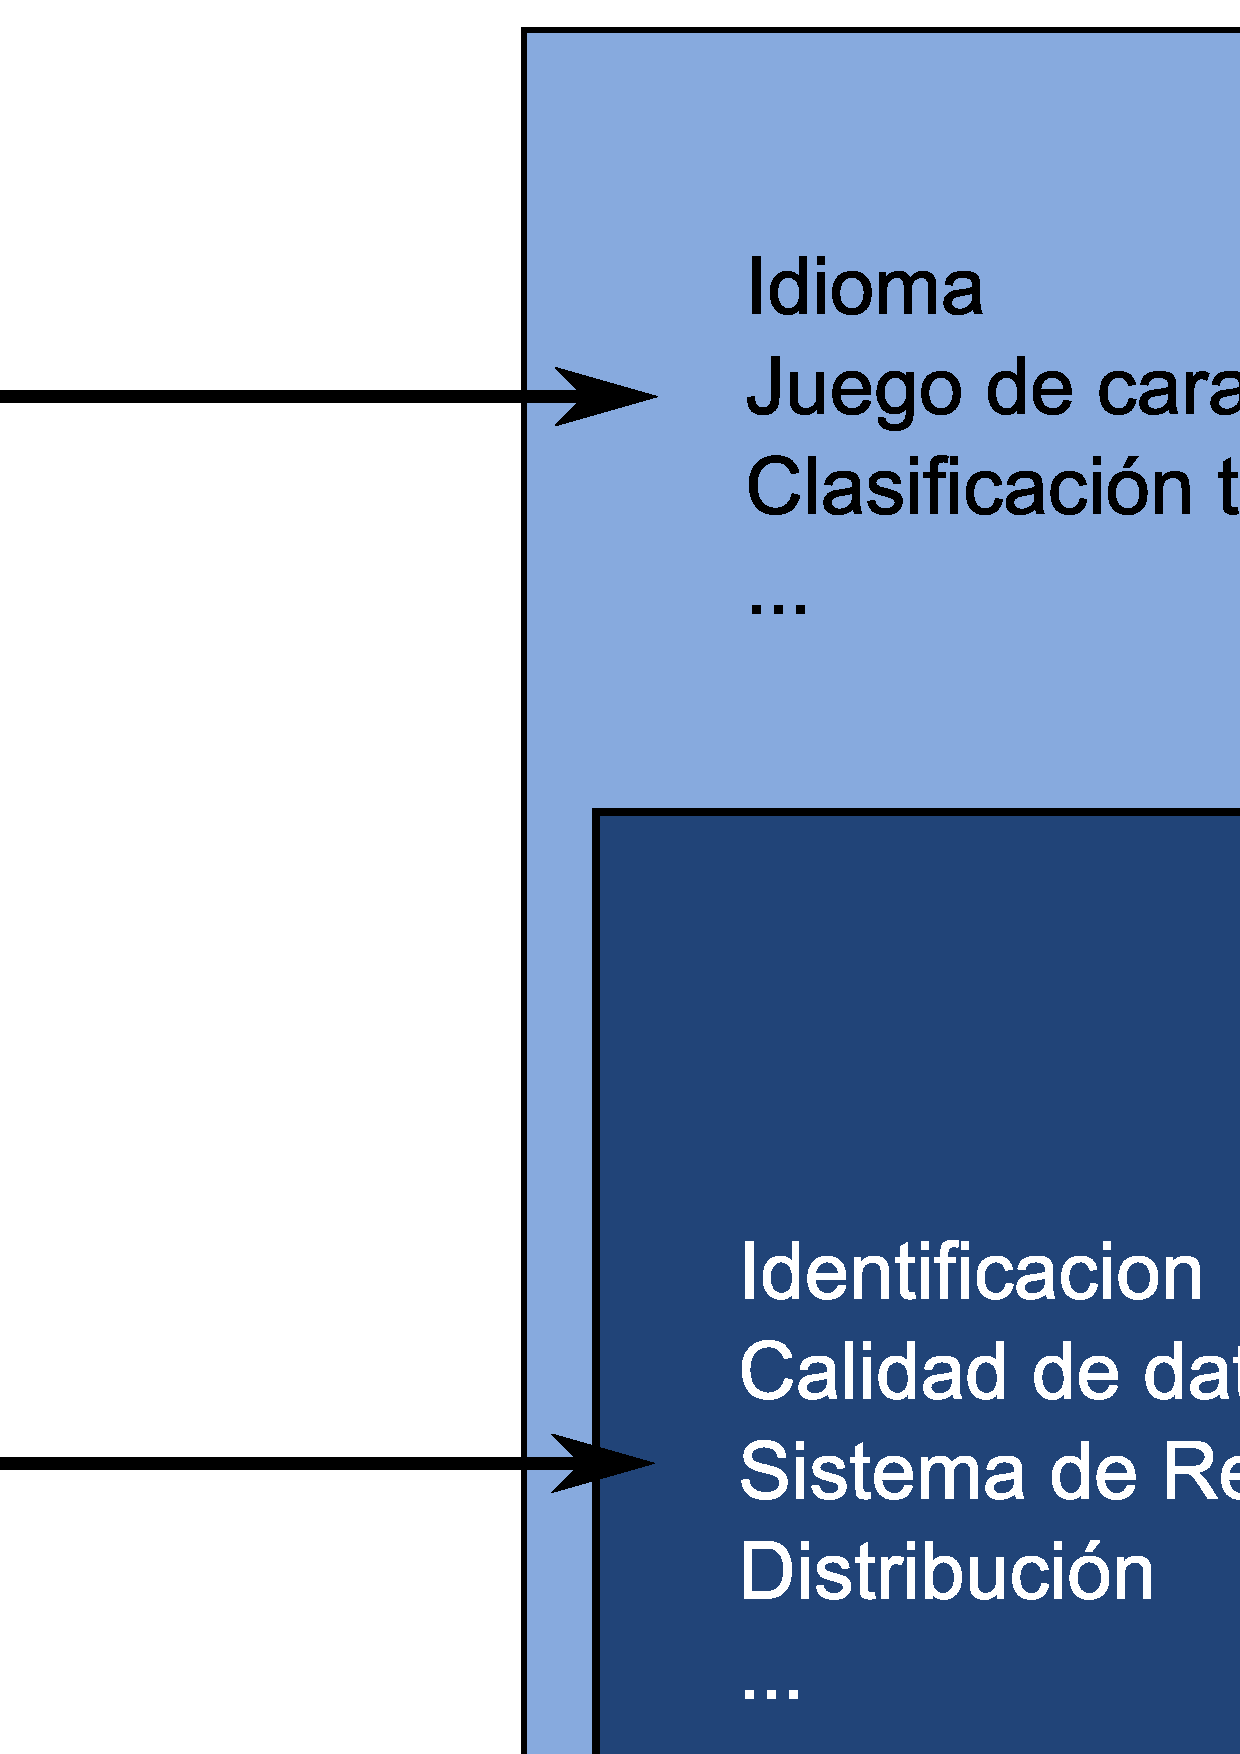
\includegraphics[width=.75\mycolumnwidth]{Metadatos/Contenido_metadatos.pdf}
%\caption{\small Los metadatos pueden presentar diferentes niveles de prioridad en su contenido.}
%\label{Fig:Contenido_metadatos} 
%\end{figure}

\subsection{Granularidad de los metadatos}

Habitualmente, los metadatos est�n asociados a un conjunto de datos al completo. Este conjunto de datos que sirve como unidad a la hora de crear metadatos coincide en general con la idea de capa en un SIG. Es decir, cada capa tiene asociado un bloque de metadatos.

 Esto no quiere decir, no obstante, que no puedan registrarse metadatos a un nivel distinto. Dependiendo del tipo de datos con los que se trabaje, puede resultar de inter�s o incluso necesario asociar metadatos a unidades distintas.

Algunos metadatos como el sistema de coordenadas ser�n compartidos por todos los elementos de una capa, y por tanto es l�gico en su caso emplear la capa como unidad b�sica en lo que a metadatos se refiere. Otro metadatos, sin embargo, hacen referencia a elementos particulares dentro de la capa.	

Este tipo de metadatos aparecen especialmente cuando a lo largo del ciclo de vida de los datos se introducen modificaciones en estos, edit�ndolos o a�adiendo nuevas entidades. Si bien en el origen el creador de los datos es una �nica entidad, otras entidades pueden alterar esos datos y deber�n actualizar correspondientemente los metadatos. Registrando como autores de los datos a ambas entidades se recoge m�s informaci�n al respecto, pero esta puede no ser suficiente. Sabemos que los datos fueron creados por una entidad A y posteriormente modificados por una entidad B, pero si tomamos un elemento dado no podemos saber si esta corresponde al trabajo original de A o a la modificaci�n realizada por B.

De modo similar, podemos incorporar a los metadatos las dos fechas de creaci�n y edici�n de los datos, as� como par�metros relativos a la calidad de los datos o las metodolog�as empleadas para recogerlos en ambos instantes. Sin embargo, no podemos saber en qu� fecha fue incorporado un elemento concreto o la calidad de los datos que definen ese elemento en particular.

En estas circunstancias, resulta m�s conveniente optar por metadatos m�s granulares, de forma que puedan recogerse particularizados para las distintas entidades de la capa.

Por ejemplo, algunos de los datos que pueden resultar de inter�s a escala de elemento (en el caso de una capa vectorial, hablamos de una geometr�a y sus atributos asociados) son los siguientes:

\begin{itemize}
\item Qui�n ha creado ese elemento.
\item Qui�n ha modificado ese elemento.
\item Cu�ndo fue creado originalmente.
\item Cu�ndo ha sido modificado por ultima vez.
\item Cu�ntas veces ha sido modificado.
\item Una descripci�n del objeto real que este elemento representa.
\end{itemize}

Podemos encontrar el caso opuesto, en el que varias capas comparten los mismos metadatos, y por tanto estos pueden asociarse a escala de toda una familia de datos. Ese es el caso cuando se tiene un conjunto de capas generadas por una misma entidad y para un mismo fin, las cuales cubren una amplia zona geogr�fica y debido a ello se encuentran divididas horizontalmente. Estas circunstancias se dan de forma habitual en series de datos de car�cter nacional o auton�mico, y conforman una de las situaciones en las que el registro de metadatos puede hacerse para toda la serie en su conjunto, al menos para algunos de esos metadatos.

\begin{figure}[!hbt]   
\centering
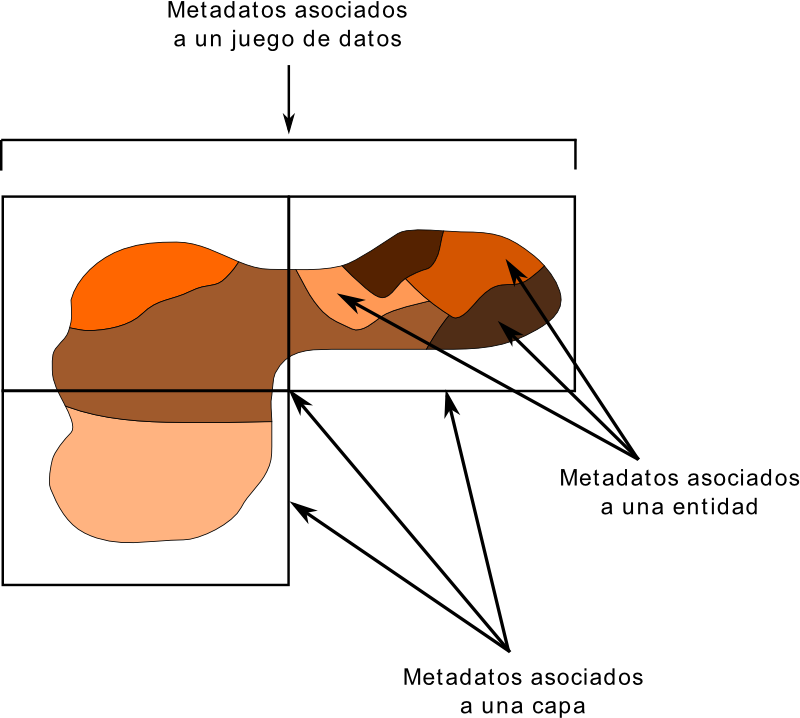
\includegraphics[width=.65\mycolumnwidth]{Metadatos/Granularidad_metadatos.pdf}
\caption{\small Granularidad de los metadatos. Los metadatos pueden hacer referencia a elementos a distinta escala.}
\label{Fig:Granularidad_metadatos} 
\end{figure}

Los metadatos pueden as� registrarse a una escala distinta a la de la capa como unidad de datos, aunque esta sigue siendo la referencia m�s habitual a la hora de crear metadatos (Figura \ref{Fig:Granularidad_metadatos}).

\subsection{Forma de almacenamiento de los metadatos}

Si para los propios datos geogr�ficos encontramos muy diversas alternativas a la hora de almacenarlos, la situaci�n no es distinta a la hora de almacenar los metadatos. Las dos alternativas principales son el uso de ficheros independientes o el almacenamiento en bases de datos \cite{metadataPrimer}.

Elegir entre uno u otro enfoque depende del conjunto de datos de trabajo, su volumen total, el uso principal que se le da o la granularidad de los datos seg�n vimos en el apartado anterior. \cite{webFGDC} recomienda el uso de bases de datos cuando los datos est�n sujetos a frecuentes modificaciones o si existe una parte de los metadatos que es com�n a varios grupos de datos. Este es el caso que vimos en el apartado anterior al mencionar los metadatos correspondiente a toda una serie de datos.

Utilizando una base de datos, resulta m�s sencillo actualizar los datos, especialmente si puede haber varios usuarios que realicen esas actualizaciones. Como veremos m�s adelante, existen servicios relacionados con la informaci�n geogr�fica que van a permitir a varios usuarios modificar un mismo juego de datos base. Las modificaciones que estos usuarios hagan han de reflejarse en los metadatos, y para ello es necesario contar con una tecnolog�a que permita un acceso concurrente similar para los metadatos. Las bases de datos proveen esas capacidades, y son por tanto adecuadas para el almacenamiento de metadatos en ese contexto.

Si, por el contrario, los datos no van a ser usados de esa forma, no es probable que deban modificarse con frecuencia y apenas contienen elementos comunes, una forma m�s simple de almacenarlos es utilizando ficheros independientes, generalmente ficheros de texto plano que son m�s sencillos de producir y adem�s pueden leerse con un simple editor de texto.

\section{Creaci�n de metadatos}

La creaci�n de los metadatos no es tarea de un �nico grupo de profesionales ni se lleva a cabo en un �nico momento dentro del ciclo de vida de los datos. Por el contrario, distintas entidades o grupos pueden crear o editar los metadatos, y pueden hacerlo a lo largo de todo el tiempo de existencia de dichos datos. 

Los metadatos puede crearse en el mismo origen de los datos, recogiendo la informaci�n al mismo tiempo que se producen los datos en s�. Esta creaci�n puede derivar de la digitalizaci�n de mapas impresos o de la medici�n directa de valores, entre otros procesos. Las organizaciones que se encargan de crear datos son responsables en este caso de crear los metadatos que los acompa�an.

Las entidades responsable de distribuir datos geogr�ficos y ponerlos a disposici�n de los distintos usuarios pueden igualmente crear metadatos en caso de que estos no existan. Estas entidades no producen datos, pero recogen datos de sus creadores y han de prepararlos para ofrecer un mejor servicio. Los metadatos aportan un valor a�adido a los datos y facilitan la gesti�n de datos que estas organizaciones han de realizar.

Por �ltimo, los mismos usuarios y beneficiarios de los datos pueden crear metadatos o ampliar los ya existentes. Si estos usuarios modifican los datos, esas modificaciones deben recogerse en los metadatos. A�n as�, incluso si no se producen modificaciones, puede resultar de inter�s a�adir nueva informaci�n en los metadatos, particularmente aquella que estos no contengan pero que pueda tener valor para los objetivos que se persiguen usando esos datos. Igualmente, dejar de usar los datos por alguna raz�n tal como el hecho de que se encuentren desactualizados es una informaci�n que los mismos usuarios pueden incorporar a los metadatos, informando as� a futuros usuarios de la falta de validez de esos datos.


En resumen, los metadatos pueden ser creados o modificados en los siguientes puntos dentro de la vida de los datos:

\begin{itemize}
\item Cuando se crean los datos.
\item Cuando se organizan o catalogan los datos.
\item Cuando se modifican o editan los datos.
\item Cuando se archivan o descatalogan los datos.
\end{itemize}

En circunstancias ideales, todo dato deber�a tener asociados unos metadatos, y estos �ltimos deber�an crearse siempre que se creen dichos datos y actualizarse siempre que estos se modifiquen. La realidad, sin embargo, es que una gran parte de los datos geogr�ficos que existen no tiene metadatos asociados, o bien estos no son lo suficientemente detallados.

Una raz�n importante para ello es la falta de concienciaci�n que existen por parte tanto de creadores de datos como de usuarios respecto a la importancia de los metadatos. Mientras que para un usuario aislado o un peque�o grupo de t�cnicos SIG puede no resultar importante generar metadatos a la hora de crear alg�n dato geogr�fico, cuando nos encontramos con organizaciones m�s grandes e infraestructuras de datos mayores los metadatos se hacen imprescindibles. El usuario aislado prefiere generalmente no dedicar tiempo (la creaci�n de metadatos no es en absoluto sencilla y es una tarea que consume tiempo) a crear unos metadatos que no percibe como importantes para su trabajo con los datos. 

Si en lugar de datos geogr�ficos habl�ramos de libros, una persona normal no cataloga los libros que tiene en su casa y recopila informaci�n acerca de cada uno de ellos, almacen�ndola en una base de datos. En una gran biblioteca, sin embargo, esta labor es imprescindible, pues de otro modo resulta imposible gestionar tanto el gran fondo bibliogr�fico del que se dispone como el amplio n�mero de lectores y usuarios.

En realidad, incluso en el nivel m�s local, las ventajas de la creaci�n de metadatos son grandes, especialmente si consideramos que un dato creado y utilizado en un entorno local puede m�s adelante pasar a formar parte de una infraestructura de datos de mayor envergadura. 

La creaci�n de metadatos no tiene que ser necesariamente una labor propia del t�cnico o equipo de t�cnicos que crean los datos en s�, del mismo modo que el escritor de un libro no es el encargado de catalogar este. Tanto usuarios como creadores de datos geogr�ficos deben poseer unos conocimientos b�sicos en relaci�n a los metadatos, pero existen expertos en metadatos a quien la creaci�n de estos debe corresponder en �ltima instancia.

Los usuarios deben saber consultar e interpretar los metadatos, y ser conscientes de la importancia de estos y el papel que juegan en una buena parte de las operaciones que pueden desarrollarse con los datos. Los creadores, por su parte, deben ser capaces de elaborar no los metadatos en s� directamente, pero s� la informaci�n necesaria acerca de los datos que debe incluirse en los metadatos, y transmitirla de forma correcta a los profesionales encargados de crear esos metadatos.

\subsection{Herramientas para crear metadatos}

Existe un amplio conjunto de herramientas que facilitan la labor de creaci�n de metadatos. Entre ellas podemos distinguir las siguientes \cite{metadataPrimer}.

\begin{itemize}
\item Editores de texto. Los metadatos pueden almacenarse en un fichero de texto plano, y por tanto pueden editarse con cualquier programa que permita la creaci�n y edici�n de tales ficheros. Lo habitual en este caso es disponer de un fichero plantilla que contenga los distintos campos que se han de registrar para cada conjunto de datos geogr�ficos, y la creaci�n del metadato consiste simplemente en apoyarse en esa plantilla y a continuaci�n de cada nombre de campo a�adir el valor correspondiente.
\item Formularios. A partir de una definici�n de campos como la anterior, se pueden desarrollar herramientas m�s elaboradas que presenten una interfaz gr�fica con distintas cajas de texto o listas desplegables. Estas aplicaciones, adem�s de ser m�s agradables para el usuario, permiten incorporar elementos de validaci�n en el proceso, evitando que en alg�n campo se introduzcan valores incorrectos o avisando al usuario en caso de que un campo presente un valor sospechoso.

Del mismo modo, se puede establecer qu� campos son obligatorios y cu�les opcionales, y avisar en caso de que un metadato no contenga valores para todos sus campos obligatorios.
\item Utilidades. Existen aplicaciones que no se emplean directamente para introducir los valores de los metadatos, pero que pueden intervenir en el proceso. Entre ellas est�n aquellas que chequean y validan los metadatos o las que lo preprocesan d�ndole un formato adecuado seg�n unas reglas establecidas de antemano.

\item Herramientas de creaci�n autom�tica de metadatos. Algunos de los valores que se incorporan a los metadatos pueden extraerse de los propios datos. Por ello, el proceso de creaci�n de metadatos puede automatizarse en cierta medida, y existen aplicaciones espec�ficamente dise�ada para realizar esa tarea.

Las aplicaciones de creaci�n autom�tica de metadatos pueden, por ejemplo, analizar un archivo con una capa vectorial y crear un archivo adjunto de metadatos en el que se incluya la extensi�n de la capa, el tipo de geometr�as que tiene o los campos de su tabla de atributos, indicando adem�s el tipo de valor en cada uno de ellos.

Adem�s de estos metadatos extra�dos directamente del dato geogr�fico, las herramientas que automatizan este proceso pueden a�adir informaci�n com�n introducida manualmente en una �nica ocasi�n, y que se repite de forma autom�tica en todos los datos creados. As�, por ejemplo, si una de estas herramientas autom�ticas se emplea en un organismo, puede establecer como creador de cada nuevo dato a esa entidad, sin necesidad de que la persona encargada de crear dicho dato deba a�adir esa informaci�n manualmente cada vez que genere algo nuevo.

El uso de herramientas autom�ticas no se limita al momento de creaci�n de los datos, sino que tambi�n pueden emplearse durante la actualizaci�n de estos. Si se actualiza un dato empleando un SIG, este puede estar conectado con la aplicaci�n de creaci�n autom�tica de metadatos y lanzar esta para que vuelva a analizar ese dato y actualizar los metadatos inmediatamente. Quiz�s sea necesario a�adir informaci�n manualmente, pero una buena parte de esta habr� sido creada de forma autom�tica, facilitando el proceso y haci�ndolo m�s r�pido.

La importancia de este tipo de aplicaciones es grande si se tiene en cuenta que, como se ha dicho, una de las razones principales de la carencia de metadatos es la cantidad de tiempo que se requiere para elaborarlos.

\end{itemize}

En el anexo \ref{Panorama_actual} veremos ejemplos de algunas de las principales herramientas existentes para el trabajo con metadatos.


\section{Algunos ejemplos}

La mejor forma de entender el contenido de los metadatos es ver algunos sencillos ejemplos reales. Puesto que estos datos son generalmente voluminosos (siempre que tengan el detalle necesario para ser realmente �tiles), en lugar de reproducirlos aqu�, puedes consultarlos en las direcciones Web \cite{ejemploMetadatos} y \cite{ejemploMetadatos2}, cada una de las cuales tiene un ejemplo concreto.

En ellas pueden verse verse los metadatos con un formato de p�gina Web sencilla compuesta de una lista de apartados y campos, as� como su valores correspondientes. A la hora de utilizar la informaci�n que estos metadatos contienen desde una aplicaci�n tal como un servidor Web, es necesario no obstante recogerlos en un formato que dicha aplicaci�n pueda entender y procesar utilizando un esquema dado y una sem�ntica bien definida. Es decir, que el \emph{software} que trabaja con metadatos no lo hace a trav�s de documentos como los de esas p�ginas Web, cuyo formato tiene como �nico fin mostrarlos de forma legible para una persona. En el cap�tulo \ref{Estandares} veremos algunos est�ndares relacionados con metadatos que definen formas estandarizadas de recoger estos para facilitar el trabajo de las aplicaciones los utilizan.

Si se comparan los campos y apartados que aparecen en ambas p�ginas, puede verse que no coinciden completamente. Eso es debido a que esos metadatos han sido generados por distintos organismos, que no utilizan una �nica metodolog�a. En el mencionado cap�tulo \ref{Estandares} veremos tambi�n que esas formas estandarizadas no solo lo son en lo referente al formato, sino tambi�n a los contenidos, con objeto de homogeneizar los metadatos generados por organizaciones distintas, proporcion�ndoles unos criterios comunes a seguir.


\section{Resumen}

Para que los datos sean verdaderamente �tiles es necesario acompa�arlos de otros datos adicionales que los describan y aporten informaci�n suplementaria acerca de ellos. Estos datos adicionales son los metadatos, y recogen informaci�n tanto de la componente espacial como de la componente tem�tica del dato geogr�fico.

La importancia de los metadatos se hace patente en la gesti�n de la calidad de los datos, o a la hora de utilizarlos como base para procesos, pues es necesario conocer todos los detalles relativos a los datos con los que se trabaja. Sin embargo, es dentro de las IDE donde los metadatos abren gran n�mero de nuevas posibilidades y se demuestran como una pieza imprescindible, ya que permiten que las operaciones de descubrimiento y consulta de los datos se efect�en de forma eficaz.

Los metadatos pueden asociarse con los datos geogr�ficos en niveles de detalle diversos, desde una �nica entidad hasta una colecci�n de varias capas. Esto permite trabajar con ellos en distintas granularidades. El contenido de los metadatos es tambi�n variable, y depende de esa granularidad, as� como de otros par�metros, como por ejemplo el tipo de datos, ya que la informaci�n adicional que puede recogerse sobre una capa vectorial no es la misma que la correspondiente a una capa r�ster.

Algunas de las secciones m�s importantes que encontramos en los metadatos son la identificaci�n del dato, los valores relativos a su calidad o los relacionados con su distribuci�n, entre otros.


%\bibliographystyle{unsrt}
%\bibliography{../../Libro_SIG}

	\chapter{Est�ndares}\label{Estandares}

\chapterauthor{Olaya, V�ctor; Turton, Ian}

\begin{keypoints}
�Qu� es un est�ndar$\bullet$�Por qu� resultan importantes los est�ndares?$\bullet$�Qui�nes se encargan de definirlos?$\bullet$�Cu�les son los principales est�ndares existentes?$\bullet$�Qu� definen esos est�ndares?$\bullet$�De qu� forma implementan los SIG los est�ndares? 
\end{keypoints}

\bigskip

\begin{intro}
Dentro de una IDE, debe ser posible acceder a los datos desde distintos puntos y hacerlo de forma simple y eficaz. Para maximizar el valor de la IDE y hacerla m�s �til para todos sus actores, es imprescindible que el acceso a los datos geogr�ficos no presente problemas. Para ello, es importante definir de forma adecuada c�mo se establece la comunicaci�n entre clientes y servidores, de forma que estos primeros no solo puedan obtener los propios datos geogr�ficos de estos �ltimos, sino tambi�n realizar consultas o conocer qu� otras funcionalidades se encuentran disponibles.

En otras palabras, resulta necesario definir una \emph{lingua franca} para que todas las comunicaciones se produzcan de forma fluida. Esto obliga a establecer una cierta normalizaci�n y crear elementos estandarizados que sean conocidos e implementados por los distintos actores de la IDE, y hacerlo para cada uno de los servicios ofrecidos, as� como para los propios datos.

En este cap�tulo veremos con detalle la importancia de los est�ndares y el papel exacto que juegan en una IDE, y describiremos una buena parte de los que actualmente existen.

Puesto que estos est�ndares est�n relacionados con las tecnolog�as cliente--servidor y las IDE, los cap�tulos correspondientes a estos elementos (cap�tulos \ref{Servidores_y_clientes_remotos} y \ref{IDEs} respectivamente) son un requisito necesario para comprender mejor el contenido de este cap�tulo.
\end{intro}

\section{Introducci�n}

En el cap�tulo \ref{Servidores_y_clientes_remotos} vimos los elementos tecnol�gicos que permiten ofrecer a trav�s de una red de servicios relacionados con la informaci�n geogr�fica. Estos servicios eran muy diversos, y ofrec�an posibilidades que iban desde obtener un dato en s� hasta la realizaci�n de consultas sobre el conjunto de operaciones que un servicio dado puede ofrecer. En todos ellos aparecen un cliente y un servidor, los cuales se comunican para realizar una tarea concreta.

Este modelo de cliente--servidor en t�rminos tecnol�gicos no es muy diferente de la idea de un cliente y un proveedor de servicios en la vida real. Una persona (el cliente) que quiera adquirir un producto de un distribuidor (el servidor) debe igualmente comunicarse con �l para preguntarle si dispone del producto deseado, realizar una petici�n de este y despu�s recibirlo cuando el distribuidor se lo env�e. En una IDE, un usuario puede consultar el cat�logo para localizar un dato concreto y despu�s acceder a �l remotamente mediante, por ejemplo, un cliente Web. Ambos esquemas de funcionamiento son muy semejantes.

Imaginemos ahora la situaci�n en la que una persona en Espa�a desea adquirir un producto electr�nico de un proveedor chino. En primer lugar, es probable que tenga dificultades para entender el cat�logo de productos, pues este describir� cada uno de ellos en chino. Si consigue localizarlo y desea adquirirlo, es igualmente probable que encuentre dificultades para comunic�rselo al proveedor, ya que seguir� existiendo la misma barrera ling��stica. Y si finalmente recibe el producto, puede tener dificultades al utilizarlo, ya que este puede funcionar a un voltaje distinto al de la red el�ctrica espa�ola o bien estar preparado para un tipo de enchufe distinto. 

Este peque�o ejemplo nos hace ver que en la relaci�n cliente--servidor pueden surgir problemas derivados de la falta de elementos comunes entre ambos actores. Si todos los elementos que toman parte en el establecimiento de esa relaci�n comercial estuvieran normalizados y fueran �nicos, un comprador de cualquier parte del mundo podr�a de forma inmediata comprar un dispositivo a cualquier vendedor de otro pa�s comunic�ndose en un �nico idioma, y tener despu�s la garant�a de poder usarlo sin problemas.

En el �mbito de la informaci�n geogr�fica la situaci�n es similar a la anterior. Hay muchos formatos distintos para almacenarla y muchas formas distintas de transmitirla, y ello dificulta el trabajo en el marco de una IDE. Igual que los clientes espa�oles no hablan el mismo idioma que los vendedores chinos, no todos los clientes SIG hablan el mismo idioma que todos los servidores, y dos cualesquiera de ellos no han de <<entenderse>> necesariamente.

De hecho, hist�ricamente los distintos fabricantes de clientes defin�an por s� mismos la forma en que sus programas se comunicaban, que no coincid�a con la del resto de fabricantes. Un cliente de un fabricante dado no podr�a acceder a los servicios de un servidor creado por un fabricante distinto. Este paradigma, caracter�stico del software privativo, es un problema en el marco de una IDE, pues dificulta el acceso a los datos.

En circunstancias ideales, en el marco de la IDE debe existir una total \emph{interoperabilidad} con independencia de los formatos y las aplicaciones empleadas, pudiendo interactuar entre s� los distintos clientes y servidores. Los est�ndares son el elemento que va a permitir esa interoperabilidad, definiendo el marco com�n que clientes y servidores emplear�n para entenderse. En un contexto altamente heterog�neo tanto en datos como en herramientas, lograr esto no resulta una tarea sencilla\cite{Lemmenes2006IEEE}, y los est�ndares son los encargados de aportar homogeneidad tecnol�gica y favorecer todo el trabajo a desarrollar dentro de una IDE. \index{Interoperabilidad}

\section{Est�ndares abiertos e interoperabilidad}

La interoperabilidad implica que podemos sustituir unos elementos del sistema en el que se incluyen los clientes y servidores por otros distintos, teniendo la seguridad de que van a interaccionar entre ellos sin dificultades. Las funcionalidades que un cliente o servidor nos ofrece pueden ser distintas a las de otro, pero independientemente de su origen (independientemente del fabricante), si esos elementos implementan un est�ndar dado, siempre podr�n interactuar con todos aquellos que tambi�n lo implementen.

La clave, por tanto, est� en los est�ndares, y en particular en que estos sean est�ndares \emph{abiertos}. Un est�ndar es un documento o pr�ctica que busca armonizar los aspectos t�cnicos de un producto o servicio. 

Un est�ndar se considera como tal cuando es empleado por un grupo o comunidad, que lo acepta para la definici�n de las caracter�sticas de ese producto o servicio en su seno. Si �nicamente es el uso del est�ndar el que lo ratifica como tal, se denomina est�ndar \emph{de facto}. El formato \emph{shapefile} para capas vectoriales, por ejemplo, es uno de estos est�ndares, ya que est� ampliamente difundido y existe tal cantidad de datos en este formato que todas las aplicaciones deben implementarlo para tener valor pr�ctico.\index{Shapefile}

Existen est�ndares que se convierten en normas o est�ndares \emph{de iure}, cuando estos son promovidos por alg�n organismo oficial de normalizaci�n o su uso se impone con car�cter legal. 

Un est�ndar \emph{abierto} es aquel cuya definici�n se encuentra disponible y todo aquel que lo desee puede conocerla y emplearla para el desarrollo de la actividad relacionada con ese est�ndar. En nuestro campo de trabajo, eso quiere decir que cualquier desarrollador que desee crear un nuevo cliente o servidor para datos SIG puede acceder al est�ndar y desarrollar en base a este.

Los principios fundamentales de los est�ndares abiertos son los siguientes \cite{perensEstandares}:

\begin{itemize}
	\item {\bfseries Disponibilidad}. Los est�ndares abiertos est�n disponibles para todos el mundo para su lectura y uso en cualquier implementaci�n.
	\item {\bfseries M�xima posibilidad de elecci�n para los usuarios finales}. Los est�ndares abiertos crean un mercado competitivo y justo, y no bloquean a los usuarios en el entorno de un vendedor particular. Desde el punto de quienes venden la tecnolog�a SIG, esto no es tan ventajoso, ya que permite la aparici�n de competidores que antes no pod�an existir. Si un fabricante basa sus productos en un est�ndar cerrado definido por �l mismo, otros no pueden elaborar soluciones que trabajen con esos productos, ya que no conocen el est�ndar empleado. 
	
	Asimismo, el fabricante puede cambiar el est�ndar utilizado por, por ejemplo, su producto de servidor, y obligar a los consumidores y a todo aquel que quiera utilizar un servicio basado en ese servidor a que actualicen tambi�n los clientes, pues los anteriores ya no podr�n comunicarse con el nuevo servidor. Utilizando est�ndares abiertos, la competencia entre fabricantes ha de basarse puramente en las capacidades que ofrecen, con lo que los consumidores ganan en calidad de los productos y en posibilidades de elecci�n.
	\item {\bfseries Gratuidad}. Implementar un est�ndar es gratuito, sin necesidad de pagar, como en el caso de una patente. Los organismos que generan los est�ndares pueden cobrar una cierta cantidad por acceder a la definici�n de los est�ndares, con objeto de financiar as� la labor que desarrollan, y tambi�n pueden cobrar por emitir certificados de que un determinado producto o servicio se ha desarrollado de acuerdo con el est�ndar.
	\item {\bfseries Discriminaci�n}. Los est�ndares abiertos y las organizaciones que los desarrollan no favorecen de ning�n modo a uno u otro implementador sobre los restantes.
	
	\item {\bfseries Extensi�n o creaci�n de subconjuntos de un est�ndar}. Los est�ndares abiertos pueden ser extendidos o bien presentados como subconjuntos del est�ndar original.
	\item {\bfseries Pr�cticas predatorias}. Los est�ndares abiertos pueden tener licencias que requieran a todo aquel que desarrolle una extensi�n de dicho est�ndar la publicaci�n de informaci�n acerca de esa extensi�n, y el establecimiento de una licencia dada para todos aquellos que creen, distribuyan y vendan \emph{software} compatible con ella. Un est�ndar abierto no puede prohibir de otro modo el desarrollo de extensiones.
\end{itemize}

Para tener una noci�n de lo que en la pr�ctica realmente significa el uso de est�ndares abiertos en el campo de los SIG y las IDE, podemos ver la figura \ref{Fig:Esquema_no_interoperable}, donde se representa el esquema de una arquitectura no interoperable. Es decir, una arquitectura que no se basa en este tipo de est�ndares.

\begin{figure}[!hbt]   
\centering
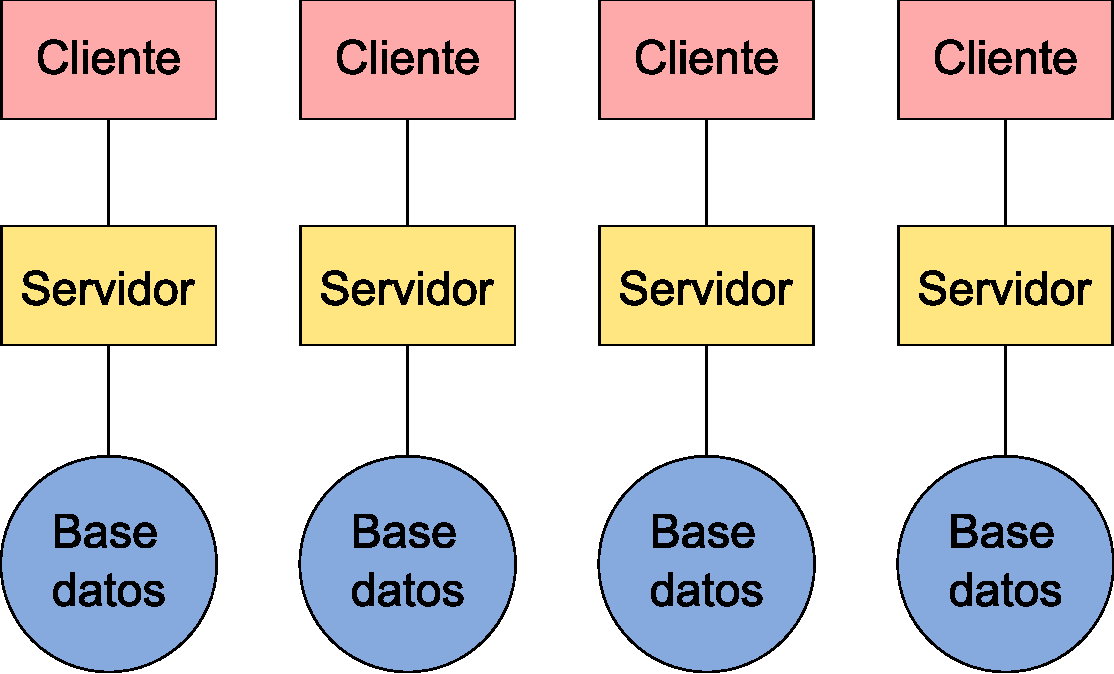
\includegraphics[width=.5\mycolumnwidth]{Estandares/Esquema_no_interoperable.pdf}
\caption{\small Esquema de una arquitectura no interoperable.}
\label{Fig:Esquema_no_interoperable} 
\end{figure}

Los datos que se encuentran en cada base de datos son accesibles �nicamente a trav�s de un �nico cliente, que es aquel correspondiente al servidor que ofrece servicios basados en esos datos. Los restantes datos quedan fuera del alcance de ese cliente, ya que no es capaz de acceder a ellos. Las diferentes soluciones cliente--servidor crean en esta situaci�n un conjunto de islas tecnol�gicas, cada una completamente independiente y sin posibilidad alguna de interactuar con las restantes.

Entre los principales inconvenientes de una arquitectura no interoperable como la representada podemos citar los siguientes:

\begin{itemize}
\item {\bfseries Desperdicio de recursos}. Cada servicio debe gestionar sus propio conjunto de datos, lo cual requiere abundantes recursos y no es sencillo, adem�s de implicar un elevado coste.
\item {\bfseries Necesidad de conocer m�ltiples clientes}. Si para acceder a cada servicio necesitamos su cliente particular, acceder al conjunto de servicios ofrecidos por esos servidores requiere por parte de los usuarios aprender a utilizar tantos clientes como servidores existan.
\item {\bfseries Imposibilidad de combinar datos}. Dos datos a los que pueda accederse a trav�s de dos servidores distintos no podr�n utilizarse simult�neamente en un �nico cliente, ya que este no podr� comunicarse con ambos servidores. Un an�lisis que requiera distintos tipos de datos no podr� realizarse si todos ellos no se ofrecen a trav�s de un mismo servidor.
\item {\bfseries Imposibilidad de combinar funcionalidades}. Los datos ofrecidos por un servidor pueden usarse para el desarrollo de muchas tareas. Estas tareas requieren que las correspondientes herramientas est�n disponibles en los clientes, y estos se diferencian notablemente, de la misma forma que lo hacen tambi�n los SIG de escritorio entre s�. Si acceder a los datos a trav�s de un servidor solo se puede hacer empleando un cliente concreto, no existe la posibilidad de aprovechar las funcionalidades de otro cliente sobre esos mismos datos, y el usuario ve as� limitadas sus posibilidades de trabajo.
\end{itemize}

En contraste con lo anterior, tenemos una situaci�n de plena interoperabilidad basada en est�ndares abiertos como la representada en el esquema de la figura \ref{Fig:Esquema_interoperable}.

\begin{figure}[!hbt]   
\centering
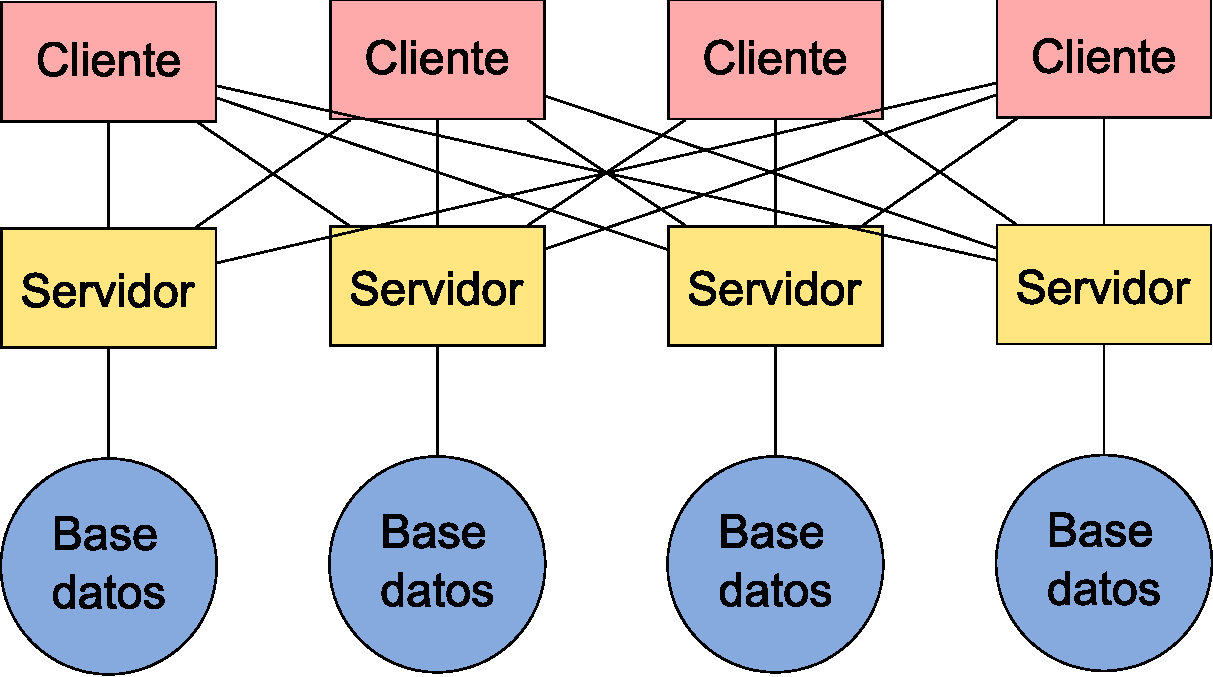
\includegraphics[width=.5\mycolumnwidth]{Estandares/Esquema_interoperable.pdf}
\caption{\small Esquema de una arquitectura interoperable.}
\label{Fig:Esquema_interoperable} 
\end{figure}

En este caso, existe un servidor que es el que gestiona y ofrece los servicios para cada base de datos, pero a �l pueden acceder todos los clientes, ya que por el hecho de estar basados en est�ndares abiertos es posible una comunicaci�n plena entre dos cualesquiera de ellos.

En esta situaci�n, un usuario puede emplear su cliente favorito (siempre que este implemente los est�ndares pertinentes) para acceder a muchos servicios distintos, o bien puede utilizar varios clientes para acceder a unos mismos datos, eligiendo en cada momento el que m�s le convenga seg�n sus necesidades. Las posibilidades de trabajo se multiplican cuando la arquitectura del sistema se fundamenta en est�ndares abiertos.

Las ventajas no son solo para los usuarios, sino tambi�n para los desarrolladores. A la hora de crear un cliente, no es necesario comprobar que este se comunica bien con todos los servidores y funciona correctamente, sino simplemente seguir las especificaciones del est�ndar. Todo aquel servidor que las implemente funcionar� sin dificultades, ya que el est�ndar garantiza la buena comunicaci�n y la interoperabilidad.

\section{Entidades creadoras de est�ndares}

Crear un est�ndar no es una labor sencilla. Se han de recoger las principales necesidades y armonizar todas ellas en una especificaci�n �nica, de modo que clientes y servidores que implementen ese est�ndar sean de la mayor utilidad posible para todos los usuarios.

Existen organizaciones dedicadas a redactar las especificaciones correspondientes a est�ndares que cubran los distintos servicios, as� como a promoverlas y mejorarlas. Los est�ndares m�s habituales en el campo de la informaci�n geogr�fica son elaborados por tres organizaciones: el Open Geospatial Consortium (OGC), ISO y W3C.

\subsection{Open Geospatial Consortium (OGC)}

El Open Geospatial Consortium \cite{webOGC} es una organizaci�n internacional y voluntaria dedicada a la elaboraci�n de est�ndares. En el OGC participan m�s de 350 organizaciones miembro, incluyendo entre ellas a los principales fabricantes del sector, agencias nacionales, grupos de investigaci�n u organizaciones sin �nimo de lucro, entre otros. Estas organizaciones miembro colaboran para alcanzar consensos y desarrollar e implementar est�ndares en el �mbito de los contenidos geoespaciales.

Algunos de los est�ndares OGC m�s relevantes, los cuales veremos a lo largo de este cap�tulo, son los siguientes:

\begin{itemize}
\item {\bfseries WMS}. Para obtener im�genes de mapas.
\item {\bfseries WCS}. Para obtener y consultar coberturas.
\item {\bfseries WFS}. Para obtener y editar entidades geogr�ficas y sus atributos asociados.
\item {\bfseries WPS}. Para servicios de procesos remotos.
\item {\bfseries GML}. Para almacenamiento de informaci�n geogr�fica.
\item {\bfseries CSW}. Para consultas en cat�logos.
\end{itemize}

Cada uno de estos est�ndares est� descrito en una especificaci�n, y estas est�n sujetas a cambios y mejoras, existiendo varias versiones en cada caso. 

%A lo largo del texto, se mencionar�n las versiones m�s recientes de cada especificaci�n, as� como las de uso e implementaci�n m�s extendida, que no necesariamente han de ser las mismas.

\subsection{ISO}

ISO \cite{webISO} es una organizaci�n internacional dedicada a la elaboraci�n de est�ndares no solo en el �mbito geogr�fico, sino en todas las �reas. ISO es responsable, por ejemplo, de est�ndares bien conocidos y aplicados en la industria actual, tales como los relacionados con la gesti�n medioambiental en empresas o los est�ndares de calidad.

Dentro de ISO existen diversos comit�s t�cnicos, cada uno de los cuales se encarga de definir los est�ndares correspondientes a un campo de trabajo. El comit� ISO/TC 211 es el responsable de aquellos relacionados con la informaci�n geogr�fica digital.

ISO redacta Especificaciones T�cnicas y Est�ndares Internacionales, catalogando estos con un n�mero que los identifica. Los elaborados por ISO/TC 211 corresponde a la serie 19100.

Existe una estrecha relaci�n entre ISO y OGC, y los est�ndares elaborados por ambas organizaciones son muchos de ellos muy similares o incluso id�nticos. De hecho, algunos de los est�ndares desarrollados por el OGC, como WMS o GML, citados anteriormente y que en breve detallaremos, son tambi�n est�ndares ISO.

En \cite{webDocsISOTC211} puede consultarse la lista de normas ISO/TC211 aprobadas y el estado de cada uno de sus documentos de trabajo.

\subsection{W3C}

El Consorcio World Wide Web (W3C) es un consorcio internacional donde las organizaciones miembro, personal a tiempo completo y el p�blico en general, trabajan conjuntamente para desarrollar est�ndares Web. Seg�n su propia definici�n\cite{webW3C}, la misi�n del W3C es \emph{guiar la Web hacia su m�ximo potencial a trav�s del desarrollo de protocolos y pautas que aseguren el crecimiento futuro de la Web}.

El W3C no guarda una relaci�n directa con los SIG, pero parece l�gico pensar que todo aquello que se haga en el seno de Internet deber�a acomodarse a las pautas establecidas por este consorcio, en especial si lo que se desea es maximizar la interoperabilidad, como ya hemos visto que resulta de inter�s en el �mbito SIG. Puesto que la mayor�a de los est�ndares abiertos que vamos a ver en este cap�tulo se aplican sobre tecnolog�as que operan en la red, estos se han de fundamentar siempre que sea posible en otros existentes desarrollados por el W3C, o al menos seguir las recomendaciones de este organismo.

Visto de otro modo, el W3C persigue objetivos similares a los de las organizaciones que elaboran est�ndares para la informaci�n geoespacial, pero su campo de actuaci�n es la red en t�rminos generales.

De entre todos los elementos definidos por el W3C, resulta de especial importancia el lenguaje XML (eXtensible Markup Language\footnote{Lenguaje de Marcado Extensible}).\index{XML} XML no es un lenguaje en s�, sino que permite definir la gram�tica de otros lenguajes. Es lo que se conoce como \emph{metalenguaje}. De este modo, puede utilizarse para definir reglas para crear formas de expresi�n que permitan recoger cualquier tipo de informaci�n. Esto hace que pueda emplearse para el intercambio de informaci�n de toda clase, y como veremos es la base de la mayor�a de est�ndares a tratar en este cap�tulo.

Entrar en detalles acerca de XML escapa del �mbito de este libro. No obstante, para aquellos que deseen saber m�s, Internet est� llena de buenas referencias libres sobre XML, como por ejemplo \cite{wikibookXML}.

\section{Est�ndares para representaci�n y obtenci�n de informaci�n geogr�fica}

Entre los est�ndares m�s importantes encontramos aquellos que especifican la forma de recoger la informaci�n geogr�fica, as� como aquellos que definen el modo en que esta se transmite.

Los siguientes est�ndares OGC forman parte de este grupo.

\subsection {Simple Features for SQL (SFS)}\label{SimpleFeatures}

Sabemos del cap�tulo \ref{Consultas} que el lenguaje SQL en su forma b�sica no sirve para recoger las geometr�as que forman la parte espacial de una entidad, sino �nicamente los datos no espaciales de esta. Sin embargo, versiones posteriores de SQL permiten la definici�n de tipos personalizados, y esto puede emplearse para poder incorporar estos elementos espaciales dentro del lenguaje.

El problema surge debido a que la propia flexibilidad de este mecanismo permite que los tipos se implementen de diversas formas, lo cual no favorece la interoperabilidad. Si una consulta se establece sobre unos tipos definidos de forma distinta a como lo est�n en la base de datos que recibe la consulta, esa consulta no podr�n procesarse correctamente. Es necesario definir una forma estandarizada de definir esos tipos, y una pauta a seguir para su implementaci�n.

OGC define la especificaci�n \extr{Simple Features for SQL} (SFS) \cite{webSFS} con objeto de hacer frente al problema anterior. SFS define por un lado unos tipos estandarizados para geometr�as, los cuales se basan en otra especificaci�n OGC denominada \extr{OpenGIS Geometry Model}, que establece una forma de definir geometr�as. Por otra parte, se definen una serie de operaciones SQL que operan sobre esos tipos.

Todas las geometr�as que pueden definirse seg�n este esquema son geometr�as en un espacio bidimensional, y cada objeto geom�trico est� asociado a un sistema de referencia en el cual se define.

Existe un objeto fundamental denominado \emph{Geometry} del que heredan los restantes en una jerarqu�a bien definida (Figura \ref{Fig:Jerarquia_clases_SFS}). Los m�todos de este objeto son de tres tipos:

\begin{itemize}
	\item M�todos b�sicos. Proveen informaci�n sobre el objeto (dimensi�n, tipo de geometr�a, sistema de referencia, etc.)
	\item M�todos para comprobar relaciones espaciales entre objetos geom�tricos (cruza a, contiene a, se intersecta con, etc.)
	\item M�todos que efect�an alg�n tipo de an�lisis (uni�n de geometr�as, distancia entre geometr�as, area de influencia de una geometr�a, etc.)
\end{itemize}

\begin{figure}[!hbt]   
\centering
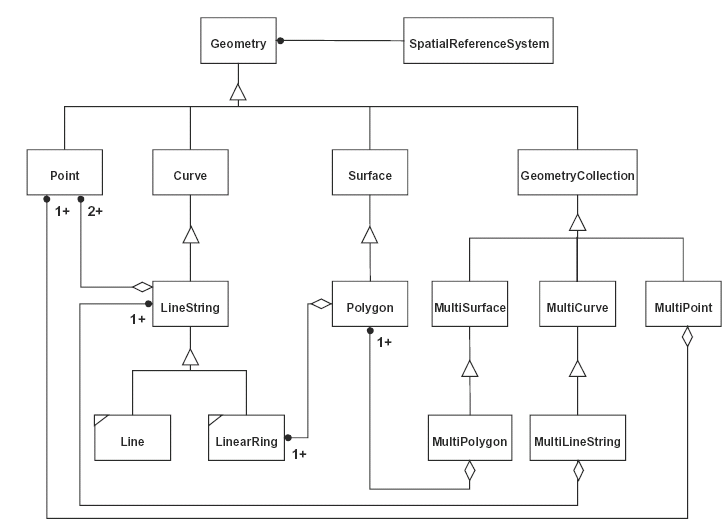
\includegraphics[width=.9\mycolumnwidth]{Estandares/Jerarquia_clases_SFS.png}
\caption{\small Esquema de clases de geometr�as en \extr{Simple Features for SQL}.}
\label{Fig:Jerarquia_clases_SFS} 
\end{figure}

Cada uno de los objetos derivados de la clase ra�z \emph{Geometry} tiene adem�s a su vez sus propios m�todos espec�ficos, siempre dentro de alguno de los grupos anteriores.

Con estos objetos y sus m�todos se da respuesta a todas las necesidades que aparecen en la realizaci�n de consultas sobre bases de datos espaciales. La especificaci�n SFS permite as� dotar de potencia al lenguaje de consulta SQL y hacerlo de forma estandarizada para ampliar la interoperabilidad en las operaciones de consulta.

\subsection {Geography Markup Language (GML)}

El \extr{Geography Markup Language} (GML) \cite{webGML} es un lenguaje basado en XML, dise�ado para el almacenamiento de informaci�n geogr�fica. Utilizando este lenguaje, resulta posible el intercambio de informaci�n geogr�fica de forma interoperable.

GML puede utilizarse para transmitir informaci�n a trav�s de una red, como parte de un servicio. Este es el caso del servicio WFS que veremos m�s adelante, que devuelve informaci�n geogr�fica codificada seg�n este lenguaje. No obstante, puede emplearse igualmente para almacenar la informaci�n con la que trabajamos de un SIG, del mismo modo que utilizamos cualquiera de los formatos de archivo que vimos en el cap�tulo \ref{Fuentes_datos}. Es decir, sin que tengan que mediar servicios en ning�n momento.

Algunos SIG permiten este uso, y soportan GML como un formato m�s de archivo. No obstante, no es una pr�ctica com�n, ya que, pese a las ventajas de ser un est�ndar aceptado, GML es un formato de fichero de tipo texto (est� basado en XML) y produce archivos de gran tama�o. Para este uso, es m�s habitual recurrir a alg�n otro formato.% , en particular aquellos que no constituyen est�ndares oficiales, pero si est�ndares \emph{de facto}, como por ejemplo el formato Shapefile (shp).

GML es un lenguaje extremadamente gen�rico, que permite recoger tanto datos r�ster como vectoriales y hacerlo con mucha flexibilidad. Permite, por ejemplo, recoger datos vectoriales sin que exista una geometr�a asociada, es decir, simplemente almacenando unos atributos como si se tratara de una base de datos no espacial. Esta gran flexibilidad, que es uno de los puntos fuertes de GML, es tambi�n uno de sus inconvenientes, ya que la especificaci�n es muy compleja y dif�cil de implementar en su totalidad.

La versi�n m�s reciente de GML es GML3, aunque GML2 es la m�s extendida.

Existe un dialecto conocido como \extr{Simple Features Protocol} que trata de solucionar el problema de la excesiva complejidad de GML3, ofreciendo las ventajas m�s importantes de este frente a GML2, pero sin incorporar todos sus elementos.

\subsection {Web Feature Service (WFS)}

El servicio \extr{Web Feature Service} WFS \cite{webWFS} est� relacionado con los datos de tipo vectorial, y a trav�s de �l se sirven directamente las entidades de un dato vectorial con sus geometr�as y datos alfanum�ricos asociados. Desde este punto de vista, acceder a un servicio WFS es similar a acceder a una capa vectorial cualquiera o a una base de datos, ya que el SIG puede recuperar la informaci�n correspondiente (tanto la componente geogr�fica como la tem�tica de cada entidad) y operar con ella.

En particular, las operaciones que permite un servicio WFS son:

\begin{itemize}
	\item Crear una nueva entidad.
	\item Borrar una entidad.
	\item Actualizar una entidad.
	\item Obtener o consultar el conjunto de entidades en base a condiciones espaciales y no espaciales.
\end{itemize}

Para realizar lo anterior, un servicio WFS debe permitir las siguientes operaciones:

\begin{itemize}
	\item \extr{GetCapabilities}. Esta operaci�n devuelve los metadatos correspondientes al propio servicio WFS. Estos contienen una descripci�n del contenido del servicio y los par�metros que este acepta a la hora de realizar peticiones sobre �l. Es decir, la respuesta a esta operaci�n es un documento que informa acerca del servicio y de los datos disponibles a trav�s de este. Este documento es un archivo XML que debe comunicar al cliente el tipo de entidades que sirve y las operaciones que soporta sobre estas.		
	\item \extr{DescribeFeatureType}. La respuesta a esta operaci�n es la descripci�n de la estructura de las entidades que pueden servirse, indicando tipo de geometr�a y nombre y tipo de campos asociados a esta.
	\item \extr{GetFeature}. Como respuesta a esta operaci�n, el servidor devuelve un conjunto de entidades. El cliente puede especificar restricciones tanto espaciales como no espaciales en los par�metros de la operaci�n, para as� limitar el conjunto de entidades obtenidas.
	
Estas entidades son devueltas por el servidor en formato GML.
	
\item \extr{Transaction}. El servidor puede realizar transacciones. Estas se componen de operaciones que modifican las entidades, tales como la creaci�n de una nueva, o la actualizaci�n o eliminaci�n de una ya existente\footnote{Recu�rdese el concepto de \emph{transacci�n} visto en el cap�tulo \ref{Bases_datos} sobre bases de datos}.
\end{itemize}

En funci�n de lo anterior, podemos distinguir dos tipos de servicios WFS:

\begin{itemize}
	\item Un servicio WFS b�sico, que solo provee las tres primeras operaciones. Es decir, que permite consultar los datos, pero no modificarlos.
	\item Un servicio WFS transaccional (WFS--T) que implementa la operaci�n de transacci�n y por tanto permite realizar modificaciones en las entidades.
\end{itemize}

La versi�n m�s actual de la especificaci�n WFS es la 1.1. No obstante, la versi�n 1.0 es la implementada mayoritariamente en los servidores actuales. WFS 1.1 utiliza GML3 como lenguaje para la codificaci�n de la informaci�n a servir, mientras que WFS 1.0 usa GML2.

\subsection{Filter Encoding}

Cuando un cliente efect�a una petici�n a un servidor WFS, no es necesario que obtenga de este todas las entidades de una capa. Incluso para una zona geogr�fica dada, el usuario puede querer obtener a trav�s del cliente solo aquellas entidades que cumplan un criterio dado. 

Ya conocemos elementos que permiten realizar ese tipo de consultas para trabajar con un subgrupo de las entidades de una capa. En el cap�tulo \ref{Consultas} vimos el lenguaje SQL, mediante el cual pod�an definirse consultas de esta clase.

El est�ndar Filter Encoding \cite{FilterEncoding} define un formato basado en XML para el almacenamiento de expresiones de filtrado seg�n otro est�ndar OGC conocido como \extr{OGC Common Catalog Query Language}. La expresi�n del filtro expresada seg�n la especificaci�n Filter Encoding puede ser validada y procesada por herramientas adicionales para convertirla en las expresiones correspondientes en otro lenguaje para consulta de bases de datos espaciales. Por ejemplo, en una clausula \texttt{WHERE} de SQL que emplear en una sentencia \texttt{SELECT}.

Las expresiones que pueden recogerse empleando \extr{Feature Encoding} pueden ser consultas con componente espacial o hacer referencia a la parte tem�tica de la informaci�n geogr�fica. Es decir, que permiten recoger toda la variabilidad de las consultas espaciales que vimos en el cap�tulo \ref{Consultas}

Adem�s de emplear estas expresiones para consultar servicios WFS, pueden utilizarse igualmente para otros como los servicios de Nomencl�tor (Gazetteer) que veremos m�s adelante, y en general en todos aquellos en los que tenga sentido especificar alg�n tipo de restricci�n a la hora de realizar una petici�n al servidor.

\subsection {Web Coverage Service (WCS)}

Si el est�ndar WFS permite obtener de un servidor datos vectoriales en forma de entidades, el est�ndar \extr{Web Coverage Service} hace lo propio con datos r�ster. Este servicio est� pensado para tratar con \emph{coberturas}, es decir, representaciones de un fen�meno que var�a en el espacio. Como ya vimos en su momento, las coberturas se corresponden con el modelos de campos.

Representar una cobertura puede hacerse de muchas formas distintas: capas r�ster, Redes de Tri�ngulos Irregulares (TIN) o funciones matem�ticas. No obstante, por el momento el est�ndar WCS solo est� preparado para el trabajo con mallas r�ster regulares.

EL servicio WCS ofrece los datos de la capa r�ster como tales, con su sem�ntica original. Es decir, que un servicio WCS puede servir un MDE y el cliente obtiene directamente los valores de elevaci�n en sus unidades correspondientes. %Despu�s ser� el cliente el que se encargue de asignarle la representaci�n que se desee para la capa obtenida, en funci�n de esos valores.

De forma similar a WFS, WCS presenta tres operaciones b�sicas que permiten consultar al servicio por sus caracter�sticas o por las caracter�sticas de los datos de que dispone, y obtener finalmente los datos en s�.

\begin{itemize}
	\item \extr{GetCapabilities}. Describe las capacidades del servicio, indicando las coberturas de que dispone.
	\item \extr{DescribeCoverage}. Describe una cobertura particular
	\item \extr{GetCoverage}. Obtiene una de las coberturas disponibles. Los par�metros de esta operaci�n se emplean para indicar al servidor la extensi�n que se desea cubrir. %, del mismo modo que en el caso de WMS.
\end{itemize}

\section{Est�ndares para mapas y visualizaci�n}

De entre todos los est�ndares que vamos a ver en este cap�tulo, los m�s importantes por ser los m�s extendidos son los que sirven mapas. Entendemos por \emph{mapa} en este contexto a una representaci�n gr�fica de una determinada informaci�n geogr�fica, elaborada a partir de una o m�s capas.

Gran parte de los sitios Web que ofrecen informaci�n geogr�fica lo hacen en forma de mapas, es decir, que permiten simplemente <<ver>> los datos geogr�ficos, y los est�ndares de esta secci�n son los encargados de definir ese tipo de servicios.

El est�ndar WMS, el principal en esta categor�a, est� ampliamente probado e implementado en gran cantidad de software, y es el soporte fundamental para cientos de aplicaciones basadas en mapas, lo que ratifica su utilidad y validez.


\subsection{Web Map Service (WMS)}

El est�ndar \extr{Web Map Service} (WMS) \cite{webWMS} define los elementos necesarios para un servicio de mapas.

Un servicio WMS devuelve una imagen con informaci�n geogr�fica, pero esta solo contiene la propia informaci�n visual para que el cliente pueda mostrarla. Es decir, si se pide a este servicio un mapa creado a partir de un MDE, la informaci�n de los p�xeles no contiene la elevaci�n de la coordenada correspondiente, sino el color asociado en funci�n de un determinado criterio. La imagen puede contener otros elementos visuales tales como etiquetas o s�mbolos, en funci�n de c�mo se haga la representaci�n en el servidor. Una vez que el cliente recibe la imagen, no puede actuar sobre esta para cambiar la forma de representaci�n de una capa, sino simplemente representarla como es.

Se definen en este servicio tres operaciones b�sicas, dos de ellas obligatorias y la restante opcional, que son empleadas por los clientes para consultar los servidores. %Junto a �sto, define el conjunto de par�metros de consulta posibles y su comportamiento asociado.

Las tres operaciones fundamentales son:

\begin{itemize}
\item \extr{GetCapabilities} (obligatoria): Al igual que en el caso de WFS y WMS, esta operaci�n describe el servicio, informando de los mapas disponibles.

\item \extr{GetFeatureInfo} (opcional): Esta operaci�n permite al cliente pedir al servidor informaci�n particular sobre algunas entidades representadas en el mapa. Si el servidor soporta esta operaci�n, los mapas que devuelve pueden consultarse. Para ello, la consulta hecha por el cliente debe a�adir ciertos par�metros adicionales como una localizaci�n (una coordenada dentro de la imagen) y el n�mero de entidades cercanas de las que se desea obtener informaci�n.

\item \extr{GetMap} (obligatoria): Esta operaci�n devuelve una imagen de un mapa con unos par�metros geoespaciales y dimensionales (tama�o de la imagen) definidos. El cliente utiliza esta funci�n para obtener un conjunto rectangular de p�xeles, los cuales conforman una imagen de un mapa correspondiente a una zona geogr�fica dada, o un conjunto de elementos gr�ficos dentro de esa zona.

La operaci�n \extr{GetMap} permite asimismo al cliente especificar qu� capas emplear para formar la imagen a obtener, el sistema de referencia a utilizar, el �rea geogr�fica a cubrir o el formato en el que se desea recibir la imagen (de entre una serie de formato habituales soportados).

Las capas pueden especificarse como accesos a otros servicios tales como WFS.
\end{itemize}

En un servicio WMS, cuando el cliente pide un mapa al servidor, puede controlar en cierto modo la forma en que este va a representarlo (colores, estilos, etc.). El servidor ofrece una serie de opciones predeterminadas, de las cuales el cliente solo conoce su nombre, y puede elegir una de ellas. No obstante, no puede saber exactamente qu� caracteriza a cada uno de esos perfiles predeterminados de representaci�n ni tampoco puede definir los suyos propios.

Para solucionar esto y ampliar las capacidades del servicio WMS, aparece otro nuevo est�ndar: SLD.

\subsection{Standard Layer Description (SLD)}\label{SLD}

El est�ndar OGC \extr{Standard Layer Description} (SLD) \cite{webSLD} define una forma de almacenar los par�metros de representaci�n empleados para crear un mapa a partir de los datos geogr�ficos. Este est�ndar permite extender las capacidades de WMS, ofreciendo al cliente la posibilidad de definir sus propias configuraciones.

SLD es un est�ndar complejo que permite cubrir situaciones variadas y no solo las m�s sencillas y habituales. Permite, por ejemplo, el ajuste de elementos tales como etiquetas o simbolog�as personalizadas para elementos puntuales (por ejemplo, representar cada punto de una capa de localizaciones de estaciones de autob�s con un peque�o dibujo de un autob�s), Para esto �ltimo se apoya en otros est�ndares tales como SVG \cite{webSVG}, dise�ado para la representaci�n de gr�ficos vectoriales.

Las simbolog�as recogidas en un documento SLD pueden emplearse para la representaci�n tanto de capas r�ster como vectoriales.

A la hora de definir una simbolog�a para una capa, es necesario conocer cierta informaci�n acerca de esta. Para definir una simbolog�a sencilla en la que todos los elementos de una capa van a ser representados de igual forma (por ejemplo, todos las l�neas de una capa de r�os con un grosor dado y en color azul), esta informaci�n no es imprescindible, pero en caso de que se quiera variar ese color o ese grosor en funci�n de un atributo, ser� necesario conocer qu� atributos tiene la capa y de qu� tipo son.

Para hacer esto, pueden emplearse las operaciones de los servicios de donde se toman los datos a representar. La operaci�n \extr{DescribeLayers} del servicio WFS permite conocer los tipos de entidades de una capa representada. La informaci�n sobre los atributos puede obtenerse con la operaci�n \extr{DescribeFeatureTypes}.

\subsection{Web Mapping Context (WMC)}

El est�ndar \extr{Web Mapping Context} (WMC) \cite{webWMC} define un formato estandarizado para almacenar un \emph{contexto}. Un \emph{contexto} recoge la informaci�n necesaria para reproducir las condiciones de una determinada sesi�n de uso de un cliente, de tal forma que ese cliente pueda restablecerlas posteriormente. El contexto se almacena en un archivo XML.

En el contexto se almacena informaci�n sobre las capas que forman el mapa representado por el cliente y los servidores de los que estas se obtienen, la regi�n cubierta por el mapa, as� como informaci�n adicional para anotar este mapa.

Los usos que se le pueden dar a un contexto son variados, entre ellos los siguientes:

\begin{itemize}
	\item Mediante un contexto se puede definir una configuraci�n particular de inicio para distintos tipos de usuario del cliente.
	\item Un contexto puede emplearse para almacenar el estado del cliente a medida que el usuario navega y modifica elementos, pudiendo retornar a una configuraci�n establecida anteriormente.
	\item El contexto puede almacenarse y despu�s transferirse a otro cliente distinto en el que comenzar en una misma configuraci�n.
\end{itemize}

Los contextos pueden a su vez catalogarse y descubrirse, ofreciendo as� un nivel de granularidad m�s amplio que las capas individuales. Pueden crearse diferentes contextos predefinidos y despu�s hacer estos accesibles para facilitar el establecimiento de una determinada configuraci�n en un cliente.

\section{Est�ndares para metadatos, cat�logos y consulta de datos}\label{estandaresCatalogos}

Los metadatos y las operaciones sobre ellos tienen sus propios est�ndares bien definidos. 

Por una parte, existen est�ndares dedicados a los metadatos en s� y a la forma de almacenarlos. Estos pueden especificar par�metros relativos a los metadatos tales como los siguientes:

\begin{itemize}
	\item Contenido de los metadatos, definiendo qu� campos son obligatorios y cu�les opcionales.
	\item Formato de almacenamiento. En general, una descripci�n del formato a emplear.
	\item Pr�cticas adecuadas de creaci�n y actualizaci�n. Se definen las pautas correctas que han de seguirse a lo largo del ciclo de vida de los datos.
	\item Reglas de conformidad. Reglas que permiten comprobar si un determinado metadato se encuentra conforme con el est�ndar.
\end{itemize}

Por otro lado, un conjunto de metadatos conforma la base para las consultas sobre un cat�logo, el cual describe a su vez un conjunto de datos. Como ya vimos, el cat�logo constituye una forma m�s sencilla y eficaz de consultar los datos, agilizando las operaciones y permitiendo el descubrimiento de datos de forma �ptima, por lo que la consulta de estos metadatos tambi�n debe estar estandarizada, y debe definirse c�mo los clientes deben obtener la informaci�n de los metadatos para posteriormente, a partir de dicha informaci�n, realizar el acceso a los datos correspondientes que resulten de inter�s.

\subsection{ISO 19115 e ISO 19119}

ISO 19115 e ISO 19119 son los est�ndares ISO para metadatos asociados a informaci�n geogr�fica. Definen m�s de 400 elementos, de los cuales los siguientes forman parte de su n�cleo fundamental.

\begin{itemize}
	\item T�tulo
	\item Fecha de referencia de los datos
	\item Idioma
	\item Categor�a en que encuadrar la tem�tica de los datos
	\item Resumen
	\item Punto de contacto para los metadatos
	\item Fecha de los metadatos
	\item Organismo responsable de los datos
	\item Localizaci�n
	\item Juego de caracteres de los datos
	\item Resoluci�n espacial
	\item Formato de distribuci�n
	\item Tipo de representaci�n espacial
	\item Sistema de referencia
	\item Recurso en l�nea
	\item Identificador del fichero de metadatos
	\item Nombre del est�ndar de metadatos
	\item Versi�n del est�ndar de metadatos
	\item Idioma de los metadatos
	\item Juego de caracteres de los metadatos
\end{itemize}

En Espa�a, existe el N�cleo Espa�ol de Metadatos (NEM), un subconjunto de la ISO 19115 definido por un subgrupo de trabajo de la IDEE.


\subsection{Nomencl�tor (Gazetteer)} \label{Nomenclator}

Un \emph{nomencl�tor} o {gazeteer} permite la localizaci�n de fen�menos geogr�ficos a partir de un determinado nombre. El cat�logo sobre el que se basa es una colecci�n de estos fen�menos, cada uno de ellos asociados a un identificador geogr�fico. Dicho identificador es una referencia espacial en forma de etiqueta o c�digo que identifica un lugar en el mundo real \cite{iso19112}. Ejemplos de tales identificadores son los nombres de ciudades o pueblos (Burgos, Plasencia), los c�digos postales (10600), los accidentes geogr�ficos (Puerto de Navacerrada, Pico de la Miel) o las direcciones (Carretera N--V p.k.35, Calle Mayor 32), entre otros. As�, el servicio de nomencl�tor permite establecer un sistema de referencia basado en identificadores geogr�ficos.

El servicio recibe como entrada un nombre y utiliza este para localizar los fen�menos geogr�ficos que cumplen un criterio. Este criterio puede ser variable, pudiendo exigir que el nombre coincida plenamente, que comience por �l, o que lo contenga, entre otras opciones. Es habitual adem�s que el cat�logo contenga una tipolog�a de los fen�menos recogidos (poblaci�n, r�o, puerto, lago, etc.), de forma que esta tambi�n puede utilizarse para establecer el criterio de consulta (por ejemplo, para localizar todos los r�os que comiencen con las letra <<b>>).

En el terreno de los nomencl�tor encontramos la Norma ISO 19115:2003 (\emph{Geographic Information -- Spatial referencing by Geographic Identifiers}), y los \emph{OGC Catalog Services}, que permiten estandarizar procesos de consulta como los mencionados.

\section{Est�ndares para procesamiento}

Adem�s de servir datos, pueden servirse procesos sobre esos datos, de tal forma que existan procesos remotos a los que los clientes pueden acceder. Tambi�n debe estandarizarse la forma de acceso a estos servicios y c�mo los clientes efectuar�n las peticiones de procesos y la transmisi�n o definici�n de los datos que han de tomarse para esos procesos.

\subsection {Web Processing Service (WPS)}

El est�ndar \extr{Web Processing Service} (WPS) de OGC est� enfocado a definir el marco en el que se ha de producir el servicio de procesos remotos. WPS define una interfaz est�ndar que facilita la publicaci�n de procesos y su uso posterior por parte de clientes. Se entiende por proceso en este contexto a todo aquel algoritmo, c�lculo o modelo que opere sobre datos georreferenciados.

Los procesos que pueden definirse son sumamente flexibles, pudiendo tener un n�mero cualquiera de entradas y salidas, y operar con distintos tipos de datos. Es decir, que ofrece un marco para definir cualquier tipo de proceso de an�lisis geogr�fico, tanto si este utiliza datos r�ster como si utiliza datos vectoriales. Todos los procesos que hemos visto en la parte \ref{Procesos} de este libro pueden ofrecerse como servicios remotos a trav�s de WPS.

Los datos empleados para alimentar los procesos pueden encontrarse en el propio servidor o ser transmitidos a trav�s de la red al igual que la propia petici�n de proceso por parte del cliente. Asimismo, puede relacionarse este est�ndar con otros que ya hemos visto, como por ejemplo WFS. Los datos necesarios para ejecutar un proceso que requiera una capa vectorial pueden obtenerse llamando a un servicio WFS, en cuyo caso debe indicarse en los par�metros del proceso los propios par�metros que corresponden a la petici�n a ese servicio WFS.

WPS define tres operaciones b�sicas, todas ellas obligatorias para todo servidor que implemente este est�ndar:

\begin{itemize}
	\item \extr{GetCapabilities}. Al igual que en otros est�ndares que ya hemos visto, esta operaci�n hace que el servidor ofrezca los metadatos referentes al servicio. En este caso, estos incluyen la definici�n de todos los procesos que es capaz de ejecutar el servidor. 
	\item \extr{DescribeProcess}. El servidor devuelve la definici�n detallada de uno de los procesos soportados, especificando n�mero y tipo de entradas y salidas, y formatos v�lidos para estas.
	\item \extr{Execute}. Esta operaci�n pide la ejecuci�n de un proceso con unas entradas dadas, y la obtenci�n de los resultados de este.
\end{itemize}

\section{Relaci�n entre est�ndares}

Los est�ndares que hemos visto a lo largo de est�s p�ginas guardan una l�gica relaci�n entre ellos. Dentro de un mismo �mbito, los est�ndares pueden guardar relaci�n con otros similares aun habiendo sido desarrollados por entidades distintas. El objetivo de armonizaci�n tecnol�gica que pretenden los est�ndares resulta m�s dif�cil de lograr si el n�mero de est�ndares para una misma tecnolog�a es elevado, ya que los fabricantes necesitan dedicar m�s tiempo y recursos a implementar todos ellos, y lo normal es que opten por implementar solo algunos.

Por este motivo, las organizaciones que promueven est�ndares trabajan conjuntamente y suelen producir est�ndares muy similares. En algunos casos, como ya hemos mencionado, algunos est�ndares OGC son tambi�n est�ndares ISO, existiendo no una similitud sino una absoluta coincidencia.

M�s importante es la relaci�n que guardan entre s� est�ndares dedicados a �reas distintas. Las tecnolog�as para la gesti�n y transmisi�n de datos  incluyen diversos elementos que forman un todo interrelacionado como vimos en el cap�tulo \ref{Servidores_y_clientes_remotos}. Los est�ndares correspondientes a esos elementos y a cada proceso particular que se desarrolla deben formar tambi�n un todo conectado y poder a su vez <<entenderse>> con otros est�ndares relacionados.

Un caso particular de esto es, por ejemplo, el de los est�ndares WMS, SLD y WFS. El servicio WMS ofrece un mapa, que no es sino una representaci�n de unos datos seg�n unos criterios dados. Esos datos pueden obtenerse de un servicio WFS y los criterios para representarlos pueden expresarse utilizando el est�ndar SLD. La ventaja de los est�ndares abiertos, m�xime si estos han sido adem�s creados por una misma organizaci�n, es la capacidad de interoperar entre ellos, de forma que WMS puede tomar datos de servicios WFS o WCS, o una consulta conforme a Filter Encoding puede aplicarse para consultar un servicio WFS y tambi�n un servicio de nomencl�tor.

Otro ejemplo en esta l�nea es el que hemos descrito para un servicio WPS que toma datos de un servicio WFS para operar con ellos.

En su conjunto deben verse todos los est�ndares como una gran familia de elementos que armoniza el trabajo con la informaci�n geogr�fica, potenciando as� el cumplimiento de los objetivos de la IDE.

%La figura \ref{Fig:Relacion_estandares_OGC} muestra de forma esquem�tica las relaciones entre algunos de los principales est�ndares OGC.
%
%\begin{figure}[!hbt]   
%\centering
%\includegraphics[width=.75\textwidth]{Metadatos/Relacion_estandares_OGC.png}
%\caption{\small Relaci�n entre algunos de los principales est�ndares OGC.}
%\label{Fig:Relacion_estandares_OGC} 
%\end{figure}

\section{Resumen}

Los est�ndares abiertos son b�sicos en el entorno de las IDE para garantizar una correcta comunicaci�n entre clientes y servidores, y su adopci�n implica una larga serie de ventajas, aumentando las posibilidades de uso de la IDE y la potencia de los datos y herramientas que se incluyen en estas.

Existen diversas organizaciones que desarrollan estos est�ndares, siendo OGC e ISO las m�s relevantes en el campo de la informaci�n geogr�fica, y W3C en el campo de la World Wide Web. Est�s organizaciones han creado est�ndares que son de aplicaci�n en diversas tareas. 

Para la codificaci�n y almacenamiento de la informaci�n geogr�fica encontramos est�ndares a nivel conceptual como SFS, y otros para la propia codificaci�n y creaci�n de archivos como GML. Este �ltimo es el empleado tambi�n para la transmisi�n de informaci�n geogr�fica seg�n el est�ndar WFS, definido para el trabajo con datos vectoriales. Para servir coberturas (en la especificaci�n actual equivalentes a datos r�ster regulares), encontramos el est�ndar WCS.

Existen igualmente est�ndares para mapas, como WMS, que a su vez se apoyan en los anteriores para obtener los datos a representar, y en otros como SLD para establecer los par�metros de esa representaci�n.

Los est�ndares se encuentra interrelacionados entre s� y se apoyan unos en otros. El conjunto de todos ellos permite en el seno de una IDE el trabajo fluido y la interoperabilidad en todas las operaciones que se realizan.

%\bibliographystyle{unsrt}
%\bibliography{../../Libro_SIG}
 





